\documentclass{book}
\usepackage[utf8]{inputenc}
\usepackage[margin=0.8in]{geometry}
%\usepackage{natbib}
%\usepackage{graphicx}
\usepackage{color}
\usepackage{amsmath}
%\usepackage{amssymb}
\usepackage{graphicx}
\usepackage{amsthm}
\usepackage{stmaryrd}
\usepackage[all]{xy}
\usepackage{multirow}
\usepackage{paralist}
\usepackage{hhline}
\usepackage{bm}
\usepackage{listings,lstcoq}
\definecolor{ltblue}{rgb}{0,0.4,0.4}
\definecolor{dkblue}{rgb}{0,0.1,0.6}
\definecolor{dkgreen}{rgb}{0,0.35,0}
\definecolor{dkviolet}{rgb}{0.3,0,0.5}
\definecolor{dkred}{rgb}{0.5,0,0}
\lstset{language=Coq}
\usepackage{pmboxdraw}
\usepackage{pifont}% http://ctan.org/pkg/pifont
\newcommand{\cmark}{\CIRCLE}%
\newcommand{\xmark}{\Circle}%
\newcommand{\hmark}{\LEFTcircle}%
\renewcommand{\matrix}[1]{\begin{bmatrix}#1\end{bmatrix}}
\usepackage{wasysym}
\usepackage{extarrows}
\usepackage{tikz}
\usetikzlibrary{positioning, shapes.geometric, graphs}
\usepackage{wrapfig}
\usepackage{dsfont}


\usepackage{amsmath}
%\usepackage{amssymb}
\usepackage{amsthm}
\usepackage{xspace}


\newtheorem{theorem}{Theorem}[section]
\newtheorem{corollary}{Corollary}[section]
\newtheorem{lemma}{Lemma}[section]
\newtheorem{remark}{Remark}[section]
\newtheorem{definition}{Definition}[section]
\newtheorem{proposition}{Proposition}[section]
\newtheorem{example}{Example}[section]
\newtheorem{problem}{Problem}[section]
\newtheorem{principle}{Principle}
\newtheorem{conjecture}{Conjecture}
\newtheorem{postulate}{Postulate}
\newtheorem{fact}{Fact}
\newtheorem{claim}{Claim}

\newtheorem{thm}{Theorem}[section]
\newtheorem{cor}{Corollary}[section]
\newtheorem{lem}{Lemma}[section]
\newtheorem{defn}{Definition}[section]
\newtheorem{prop}{Proposition}[section]
\newtheorem{exam}{Example}[section]
\newtheorem{conj}{Conjecture}
\newtheorem{clm}{Claim}


\newcommand {\nat } {{\mathbb{N}}}
\newcommand {\complexnumber } {{\mathbb{C}}}
\newcommand {\real } {{\mathbb{R}}}
\newcommand {\bI } {{\mathbf{I}}}
\newcommand {\bi } {{\boldsymbol{i}}}

\newcommand {\bB } {{\mathbb{B}}}
\newcommand {\bN } {{\mathbb{N}}}
\newcommand {\bC } {{\mathbb{C}}}
\newcommand {\bR } {{\mathbb{R}}}
\newcommand {\bQ } {{\mathbb{Q}}}
\newcommand {\bZ } {{\mathbb{Z}}}
\newcommand {\bF } {{\mathbb{F}}}
\newcommand {\bt } {{\mathbf{t}}}
\newcommand {\bu } {{\mathbf{u}}}
\newcommand {\bv } {{\mathbf{v}}}
\newcommand {\bw } {{\mathbf{w}}}

\newcommand {\qbar} {{\overline{q}}}
\newcommand {\qI} {{q:=|0\rangle}}
\newcommand {\qU} {{\overline{q}:=U[\overline{q}]}}
\renewcommand{\bra}[1]{\langle #1|}
\renewcommand{\ket}[1]{|#1\rangle}
\renewcommand{\braket}[3]{\langle #1|#2|#3\rangle}

\newcommand {\cA } {{\mathcal{A}}}
\newcommand {\cB } {{\mathcal{B}}}
\newcommand {\cC } {{\mathcal{C}}}
\newcommand {\cD } {{\mathcal{D}}}
\newcommand {\cE } {{\mathcal{E}}}
\newcommand {\cF } {{\mathcal{F}}}
\newcommand {\cG } {{\mathcal{G}}}
\newcommand {\cH } {{\mathcal{H}}}
\newcommand {\cI } {{\mathcal{I}}}
\newcommand {\cJ } {{\mathcal{J}}}
\newcommand {\cK } {{\mathcal{K}}}
\newcommand {\cL } {{\mathcal{L}}}
\newcommand {\cM } {{\mathcal{M}}}
\newcommand {\cN } {{\mathcal{N}}}
\newcommand {\cO } {{\mathcal{O}}}
\newcommand {\cP } {{\mathcal{P}}}
\newcommand {\cQ } {{\mathcal{Q}}}
\newcommand {\cR } {{\mathcal{R}}}
\newcommand {\cS } {{\mathcal{S}}}
\newcommand {\cT } {{\mathcal{T}}}
\newcommand {\cU } {{\mathcal{U}}}
\newcommand {\cV } {{\mathcal{V}}}
\newcommand {\cW } {{\mathcal{W}}}
\newcommand {\cX } {{\mathcal{X}}}
\newcommand {\cY } {{\mathcal{Y}}}
\newcommand {\cZ } {{\mathcal{Z}}}
\newcommand {\cSO} {{\mathcal{SO}}}
\newcommand {\cQO} {{\mathcal{QO}}}
\newcommand {\cQC} {{\mathcal{QC}}}
\newcommand {\cCP} {{\mathcal{CP}}}
\newcommand {\id } {{I}}
\renewcommand {\i } {{\boldsymbol{i}}}
\newcommand {\bD} {{\mathbf{D}}}
\newcommand{\cg}[1]{{{\color{purple}\left\{{\color{black}#1}\right\}}}}
\newcommand{\cgrule}[5]{{{\color{purple}\models}_{#1}^{#2}\cg{#3}{#4}\cg{#5}}}
%\newcommand{\Mexist}{\downmapsto}

%\DeclareRobustCommand{\Mexist}{\,\mathbin{\ooalign{$\downarrow$\cr\hss\raisebox{1.15ex}{\hspace{-0.925ex} \scriptsize $-$}\hss}}\,}

\newcommand {\doms } {{\mathsf{dom}}}
\newcommand {\dom }[1] {{\mathsf{dom}\!\left(#1\right)}}
\newcommand {\codom }[1] {{\mathsf{codom}\!\left(#1\right)}}
\newcommand {\codoms }[1] {{\mathsf{codom}}}
\newcommand {\frees } {{\mathsf{free}}}
\newcommand {\free }[1] {{\mathsf{free}\left(#1\right)}}
\newcommand {\ptype} {{\mathrm{type}}}
\newcommand {\res} {{\mathrm{Res}}}
\newcommand {\emptyprog} {{\mathbf{E}}}
\newcommand{\downmapsto}{\rotatebox[origin=c]{-90}{$\scriptstyle\mapsto$}\mkern2mu}
\newcommand {\rt }[2] {{\left.{#1}\right|_{#2}}}
\newcommand {\tr } {{\mathrm{tr}}}
\newcommand{\rank}{{\rm rank}}
\newcommand {\sem}[1] {\llbracket#1\rrbracket}
\newcommand {\lsem}[1] {\llbracket#1\rrbracket_l}
\newcommand {\coqm}[1] {\text{\small\ttfamily{#1}}}
\newcommand{\mx}{{{\tt x}}}
\newcommand{\my}{{{\tt y}}}
\newcommand{\mz}{{{\tt z}}}
\newcommand{\mt}{{{\tt t}}}
\newcommand{\ms}{{{\tt s}}}
\newcommand{\mF}{{{\tt F}}}
\newcommand{\mT}{{{\tt T}}}
\newcommand{\mi}{{{\tt i}}}
\newcommand{\mj}{{{\tt j}}}
\newcommand{\mk}{{{\tt k}}}
\newcommand{\mm}{{{\tt m}}}
\newcommand{\mn}{{{\tt n}}}
\renewcommand{\mp}{{{\tt p}}}
\newcommand{\mq}{{{\tt q}}}
\newcommand{\mr}{{{\tt r}}}
\newcommand{\wf}{{\mathcal{WF}}}
\newcommand {\seml}[1] {\llparenthesis#1\rrparenthesis}
\newcommand {\spans } {{\mathrm{span}}}
\newcommand {\spec} {{\mathrm{spec}}}
% \newcommand {\dim } {{\mathrm{dim}}}
\newcommand {\supp } {{\mathrm{supp}}}
\newcommand {\cspan } {{\overline{\mathrm{span}}}}
\newcommand {\ol}[1] {{\overline{#1}}}
\newcommand {\ob}[2] {{\left.{#1}\right|_{#2}}}
%\newcommand{\msd}[1][fill=black]{\tikz [x=1ex,y=1ex,line width=.01ex,line join=round] \draw[transform canvas={yshift=.0133cm}]  [#1]  (0,0.5) -- (0.5,1) -- (1,.5) -- (.5,0) -- (0,.5) -- cycle;}%
\def\>{\ensuremath{\rangle}}
\def\<{\ensuremath{\langle}}
\def\ra{\ensuremath{\rightarrow}}
\def\Ra{\ensuremath{\Rightarrow}}
\def\la{\ensuremath{\longleftarrow}}

\newcommand {\swap} {\mathrm{SWAP}}
\newcommand{\proj}{{\mathrm{proj}}}
\newcommand{\op}[1]{{\operatorname{#1}}}
\DeclareTextCommand{\tus}{OT1}{%
  \leavevmode \kern.06em\vbox{\hrule width.6em}}
\newcommand{\us}{{\text{\tus}}}
\newcommand{\tb}{{\text{\textbar}}}
\newcommand{\qerr}{{\mathbf{err}}}
\newcommand{\terr}{{\mathbf{terr}}}
\newcommand{\err}{{\textbf{err}\xspace}}
\newcommand{\scalar}{\textbf{scalar}\xspace}
\newcommand{\suptype}{{\textsf{supertype}\xspace}}
\newcommand{\type}{{\textsf{type}\xspace}}

\newcommand{\vzero}[1]{{\mathbf{0}_{#1}}}
\newcommand{\ozero}[2]{{\mathbf{0}_{#1\rightarrow#2}}}
\newcommand{\idfun}[1]{{\mathds{1}_{#1}}}
\newcommand{\perm}[2]{{\mathbf{Perm}_{#1\rightarrow#2}}}

\providecommand{\TODO}[1]{{\protect\color{red}\noindent {\bf [TODO]}\emph{#1} {\bf [/TODO]}}}
\providecommand{\todo}[1]{{\protect\color{red}\noindent {\bf [todo]}\emph{#1} {\bf [/todo]}}}

\renewcommand{\tt}[1]{\texttt{\frenchspacing{#1}}}
\newcommand{\bs}{{\textbackslash}}

\newcommand{\kskip}{{\mathbf{skip}}}
\newcommand{\kif}{{\mathbf{if}}}
\newcommand{\kwhile}{{\mathbf{while}}}
\newcommand{\kfi}{{\mathbf{fi}}}
\newcommand{\ido}{{\mathbf{do}}}
\newcommand{\iod}{{\mathbf{od}}}
\newcommand{\iskip}{{\mathbf{skip}}}
\newcommand{\iinit}[1]{{{#1} := |0\>}}
\newcommand{\iunit}[2]{{{#1} := {#2}[{#1}]}}
\newcommand{\icond}[4]{{\mathbf{if}\ {#2}[{#3}] = {#1}\rightarrow{#4}_{#1}\ \mathbf{fi}}}
\newcommand{\iwhile}[4]{{\mathbf{while}\ {#1}[{#2}] = {#3}\ \mathbf{do}\ {#4}\ \mathbf{od}}}
\newcommand{\rname}[1]{\textrm{({#1})}}
\newcommand{\iconf}[2]{{\<{#1},\ {#2}\>}}
\newcommand{\cf}[3]{{\left\{#2\right\}#1\left\{#3\right\}}}
\newcommand{\aabort}{{\mathbf{abort}}}
\newcommand{\askip}{{\mathbf{skip}}}
\newcommand{\pset}[1]{{\text{\textrm{set}}({#1})}}
\newcommand{\ainit}[1]{{\mathbf{init}\ {#1}}}
\newcommand{\aapply}[1]{{\mathbf{apply}\ {#1}}}
\newcommand{\acond}[3]{{\mathbf{if}\ (\square{#1}\cdot{#2} = {#1}\rightarrow{#3}_{#1})\ \mathbf{fi}}}
\newcommand{\awhile}[3]{{\mathbf{while}\ {#1} = {#2}\ \mathbf{do}\ {#3}\ \mathbf{od}}}
\newcommand{\akwhile}[4]{{\mathbf{while}^{(#4)}\ {#1} = {#2}\ \mathbf{do}\ {#3}\ \mathbf{od}}}
\newcommand{\afor}[3]{{\mathbf{for}\ {#1}{#2}\ \mathbf{do}\ {#3}_{#1}}}
\newcommand{\CtoQE}{{\texttt{\%:QE}}}
\newcommand{\cl}{{{cl}}}
\renewcommand{\imath}{\mathbf{i}}
\newcommand{\ul}{{\underline{~~}}}

\def\lb{\ensuremath{\llbracket}}
\def\rb{\ensuremath{\rrbracket}}

\newcommand{\gb}[1]{\textit{\color{green}[GB] : #1}}
\newcommand{\py}[1]{\textit{\color{red}[PY] : #1}}
\newcommand{\lz}[1]{\textit{\color{blue}[LZ] : #1}}
\newcommand{\jl}[1]{\textit{\color{blue}[JL] : #1}}
\newcommand{\yx}[1]{\textit{\color{blue}[YX] : #1}}

\newcommand{\modify}[1]{{\color{red}#1}}

\usepackage{amssymb}
\usepackage{amsmath}
\usepackage{stmaryrd}
\usepackage{hyperref}

\usepackage{braket}


\title{\textbf{Dirac Notation Theories}\\ 
\Large{Infrastructure for Quantum Formal Systems}}
\author{}

\begin{document}

\maketitle

\tableofcontents

% \clearpage

% 
\section{Quantum Variable}

For array, we first support one-dimensional (dependent) array, i.e., tuple, ffun, and dffun.

\begin{itemize}
    \item $L$ : set of labels. Used to indicate quantum systems/quantum variables.
    \item $S\subseteq L$ : subsystems.
    \item \coqe{qvar := seq nat}.
    \item context: $\Gamma : \coqm{qvar}\rightarrow\coqm{option ihbFinType}$.
    If $\Gamma\ \mx = \coqm{Some}\ \mT$, we write $\Gamma\vdash \mx : \mT$, and say $\mx\in\Gamma$.
    \item Declaration for quantum variables: 
    
    \coqe{declare x : qvar T}
    $$\frac{\mx : \bN\quad \mx\notin\Gamma\quad\mT:\coqm{ihbfinType}\quad\coqm{declare}\ \mx : \coqm{qvar}\ \mT}{\Gamma\ [::\mx] = \coqm{Some}\ \mT}$$
    
    
    \coqe{declare x : qtuple n T}
    $$\frac{\mx,n: \bN\quad\mx\notin\Gamma\quad\mT:\coqm{ihbfinType}\quad\coqm{declare}\ \mx : \coqm{qtuple}\ n\ \mT}{\Gamma\ \mx = \coqm{Some}\ \coqm{n.-tuple}\ \mT,\quad \forall\,\mi:\coqm{'I\_n}, \Gamma\ [::\mx,\coqm{enum\_rank}\ \mi] = \coqm{Some}\ \mT}$$
    
    \coqe{declare x : qffun F T}
    $$\frac{\mx : \bN\quad\mF:\coqm{finType}\quad \mx\notin\Gamma\quad\mT:\coqm{ihbfinType}\quad\coqm{declare}\ \mx : \coqm{qffun}\ \mF\ \mT}{\Gamma\ \mx = \coqm{Some}\ \{\coqm{ffun F $\rightarrow$ T}\},\quad \forall\,\mi:\mF, \Gamma\ [::\mx,\coqm{enum\_rank}\ \mi] = \coqm{Some}\ \mT}$$
    
    \coqe{declare x : qdffun T}
    $$\frac{\mx : \bN\quad\mF:\coqm{finType}\quad \mx\notin\Gamma\quad\mT:\mF\rightarrow\coqm{ihbfinType}\quad\coqm{declare}\ \mx : \coqm{qdffun}\ \mT}{\Gamma\ \mx = \coqm{Some}\ \{\coqm{dffun $\forall$\,i\,:\,F, T i}\},\quad \forall\,\mi:\mF, \Gamma\ [::\mx,\coqm{enum\_rank}\ \mi] = \coqm{Some}\ \mT\ \mi}$$
    \item For any declared $\mx : \coqm{qvar}$, $\pset{\mx}\subseteq L$ gives the corresponding quantum subsystem of $\mx$.
    \item Compute disjointness of \coqe{x y : qvar}:
    \begin{coq}
    Fixpoint qvar_dis (x y : qvar) : bool :=
        match x,y with
        | Nil, _ => false
        | _, Nil => false
        | [:: hx], [:: hy] => hx != hy
        | hx :: tx, hy :: ty => if (hx == hy) then qvar_dis tx ty
                                else true
        end.
    Fixpoint qvar_dis_seq (x : qvar) (s : seq qvar) : bool :=
        match s with
        | Nil => true
        | h :: t => if qvar_dis x h then qvar_dis_seq x t else false
        end.
    Fixpoint qvar_seq_dis (s : seq qvar) : bool :=
        match s with
        | Nil => true
        | h :: t => if qvar_dis_seq h t then qvar_seq_dis t else false
        end.
    \end{coq}
    \item Assumption: $\forall\,\mx\ \my:\coqm{qvar}$ such that $\mx,\my\in\Gamma$, then $\coqm{qvar\_dis x y} = [\coqm{disjoint}\ \pset{\mx}\ \&\ \pset{\my}]$.
    \item quantum register? Question: how to composite variables? How to automatically derive the type? (i.e., $\Gamma\vdash (\mx,\my) : \mT_1\ast\mT_2 $).
\end{itemize}

\section{Dirac Notation}

\begin{definition}[syntax]
    We here consider the Dirac expressions inductively generated by:
    $$e ::= c\CtoQE\ \Big|\ |v\>_\mx\ \Big|\ {}_\mx\<v|\ 
    %\Big|\ M[\mx]\ 
    \Big|\ M[\mx,\my]\ \Big|\ e^\dag\ \Big|\ e^T\ \Big|\ e^\ast\ \Big|\ e + e\
    \Big|\ c \star e \ \Big|\ e \circ e\ \Big|\ e \cdot e\ \Big|\ e\otimes e\ \Big|\ \sum_i e_i$$
    %\ \Big|\ \prod_i e_i\ \Big|\ \bigotimes_i e_i$$
    where $c\in\complexnumber $ and the index $i$ of summation is over some $\coqm{finType}$ (unconditional). $c \star e$ is the scale operator.
    If $\Gamma\ x = \coqm{Some}\ \mT_\mx$ and $\Gamma\ y = \coqm{Some}\ \mT_\my$, then $v\in\cH_{\mT_\mx}$ and $M\in\cL(\cH_{\mT_\mx},\cH_{\mT_\my})$ (if $\mx = \my$, we write it as $M[\mx]$). 
    
    Notation: we write $M[\mx]$ for $M[\mx,\mx]$ and  $|v\>_\mx\<u|$
    for outer product $(|v\>\<u|)[\mx]$.
    
    Question: constant? $0\CtoQE, 1\CtoQE, {\bf 0}_S, {\bf 0}_{S,T}, I_S$?
\end{definition} 

\begin{definition}[type]
	For each well-formed Dirac expression $e$, it has a domain $S$ and a codomain $S^\prime$. We write $\vdash e : (S,S^\prime)$. Following are the typing rules:
	\begin{align*}
		\frac{}{\vdash c\CtoQE : (\emptyset, \emptyset)} \qquad
		\frac{}{\vdash |v\>_\mx : (\emptyset, \pset{\mx})} \qquad
		\frac{}{\vdash {}_\mx\<v| : (\pset{\mx},\emptyset)} \\
		\frac{}{\vdash M[\mx,\my] : (\pset{\mx}, \pset{\my})} \qquad
		\frac{\vdash e : (S,S^\prime)}{\vdash e^\dag : (S^\prime, S)} \qquad
		\frac{\vdash e : (S,S^\prime)}{\vdash e^T : (S^\prime, S)} \qquad
		\frac{\vdash e : (S,S^\prime)}{\vdash e^\ast : (S, S^\prime)} \qquad \\
		\frac{\vdash e_1 : (S,S^\prime)\quad\vdash e_2 : (S,S^\prime)}{\vdash e_1+e_2 : (S,S^\prime)}\qquad
		\frac{\vdash e : (S,S^\prime)}{\vdash c\star e : (S,S^\prime)}\qquad
		\frac{\vdash e_1 : (S^\prime,S^{\prime\prime})\quad\vdash e_2 : (S,S^\prime)}{\vdash e_1\circ e_2 : (S,S^{\prime\prime})}\\
		\frac{\vdash e_1 : (S_1,S_1^{\prime})\quad\vdash e_2 : (S_2,S_2^{\prime})\quad [\coqm{disjoint}\ S_1\ \&\ S_2-S_1^\prime] \quad [\coqm{disjoint}\ S_2^\prime\ \&\ S_1^\prime-S_2]}{\vdash e_1\cdot e_2 : (S_1\cup(S_2-S_1^\prime), S_2^\prime\cup(S_1^\prime-S_2)}\\
		\frac{\vdash e_1 : (S_1,S_1^{\prime})\quad\vdash e_2 : (S_2,S_2^{\prime})\quad [\coqm{disjoint}\ S_1\ \&\ S_2] \quad [\coqm{disjoint}\ S_1^\prime\ \&\ S_2^\prime]}{\vdash e_1\otimes e_2 : (S_1\cup S_2, S_1^\prime\cup S_2^\prime)}\qquad
		\frac{\forall\,i,\ \vdash e_i: (S,S^\prime)}{\vdash\sum_ie_i:(S,S^\prime)}
	\end{align*}
	Conversely, for any Dirac expression $e$, if there are $S, S^\prime$ such that $\vdash e : (S,S^\prime)$, we say $e$ is well-formed and write $\vdash \wf(e)$.
\end{definition}

\begin{definition}[simplification]
	We write $C\vdash e\ra e^\prime$ for simplification. That is, $e$ can be replaced by $e^\prime$ if the side condition $C$ holds (since we only consider well-formed expressions, the conditions $\wf(e)$ and $\wf(e^\prime)$ are always necessary and thus omitted from $C$). 
	Following are basic simplification rules:
\end{definition}
\begin{align*}
	\text{Associativity:}\quad
	&\vdash e_1 + (e_2 + e_3) \ra e_1 + e_2 + e_3 \quad
	\vdash e_1 \circ (e_2 \circ e_3) \ra e_1 \circ e_2 \circ e_3 \\
	&\vdash e_1 \cdot (e_2 \cdot e_3) \ra e_1 \cdot e_2 \cdot e_3 \quad
	\vdash e_1 \otimes (e_2 \otimes e_3) \ra e_1 \otimes e_2 \otimes e_3\\
	\text{Commutativity:}\quad
	&\vdash e_1 + e_2 \ra e_2 + e_1 \quad
	\vdash e_1 \otimes e_2 \ra e_2 \otimes e_1 \\
	\text{Distributivity:}\quad
	&\vdash e \circ (e_1 + e_2) \ra e \circ e_1 + e \circ e_2\quad
	\vdash (e_1 + e_2) \circ e \ra e_1 \circ e + e_2 \circ e\\
	&\vdash e \cdot (e_1 + e_2) \ra e \cdot e_1 + e \cdot e_2\quad
	\vdash (e_1 + e_2)\cdot e \ra e_1 \cdot e + e_2 \cdot e\\
	&\vdash e \otimes (e_1 + e_2) \ra e \otimes e_1 + e \otimes e_2\quad
	\vdash (e_1 + e_2) \otimes e \ra e_1 \otimes e + e_2 \otimes e\\
	\text{Identity:}\quad
	&\vdash 0\CtoQE + e \ra e\quad \vdash e + 0\CtoQE \ra e \quad
	\vdash {\bf 0}_{S,T} + e \ra e\quad \vdash e + {\bf 0}_{S,T} \ra e \\
	&\vdash I_S\circ e \ra e\quad \vdash e\circ I_S \ra e\\
	&\frac{\vdash e : (S,S^\prime)}{\vdash e \otimes {\bf 0}_{T,T^\prime} \ra 
		{\bf 0}_{S\cup T,S^\prime\cup T^\prime}}\quad
	\frac{\vdash e : (T,T^\prime)}{\vdash {\bf 0}_{S,S^\prime} \otimes e \ra 
		{\bf 0}_{S\cup T,S^\prime\cup T^\prime}}\\
	&\frac{\vdash e : (S,S^\prime)}{\vdash e \circ {\bf 0}_{T,S} \ra 
		{\bf 0}_{T,S^\prime}}\quad
	\frac{\vdash e : (S,S^\prime)}{\vdash {\bf 0}_{S^\prime,T}\circ e \ra 
		{\bf 0}_{S,T}}\\
	&\frac{\vdash e : (S,S^\prime)}{\vdash e \cdot {\bf 0}_{T,T^\prime} \ra 
		{\bf 0}_{S\cup(T-S^\prime), T^\prime\cup(S^\prime-T)}}\quad
	\frac{\vdash e : (T,T^\prime)}{\vdash {\bf 0}_{S,S^\prime}\cdot e \ra 
		{\bf 0}_{S\cup(T-S^\prime), T^\prime\cup(S^\prime-T)}}\\
	\text{Scalar:}\quad
	&\frac{\vdash e : (S,S^\prime)}{\vdash 0\CtoQE \star e \ra {\bf 0}_{S,S^\prime}} \quad \vdash 1\CtoQE \star e \ra e \quad 
	\vdash I_{\emptyset} \ra 1\CtoQE
	\\ 
	&\vdash c\CtoQE \circ e \ra c\CtoQE \star e \quad \vdash c\CtoQE \cdot e \ra c\CtoQE \star e \quad \vdash c\CtoQE \otimes e \ra c\CtoQE \star e\\
	&\vdash c\CtoQE^\dag \ra \overline{c}\CtoQE \quad
	\vdash c\CtoQE^\ast \ra \overline{c}\CtoQE \quad
	\vdash c\CtoQE^T \ra c\CtoQE \\
	&c_1\CtoQE \star e + c_2\CtoQE \star e \ra (c_1+c_2)\CtoQE \star e \quad
	c_1\CtoQE \star (c_2\CtoQE \star e) \ra (c_1c_2)\CtoQE \star e\\
	&c\CtoQE \star (e_1 + e_2) \ra c\CtoQE \star e_1 + c\CtoQE \star e_2\\
	&(c_1\CtoQE \star e_1)\circ e_2 \ra c_1\CtoQE \star(e_1\circ e_2)\quad 
	e_1\circ (c_2\CtoQE \star e_2)\ra c_2\CtoQE \star(e_1\circ e_2)\\ 
	&(c_1\CtoQE \star e_1)\cdot e_2 \ra c_1\CtoQE \star(e_1\cdot e_2)\quad 
	e_1\cdot (c_2\CtoQE \star e_2)\ra c_2\CtoQE \star(e_1\cdot e_2)\\ 
	&(c_1\CtoQE \star e_1)\otimes e_2 \ra c_1\CtoQE \star(e_1\otimes e_2)\quad 
	e_1\otimes (c_2\CtoQE \star e_2)\ra c_2\CtoQE \star(e_1\otimes e_2)\\
	\text{Inner/Outer product:}\quad
	&{}_S\<u|\circ |v\>_S \ra \<u|v\>\CtoQE \quad 
	{}_S\<u|\cdot |v\>_S \ra \<u|v\>\CtoQE \quad
	\<\mt_1|\circ |\mt_2\> \ra \delta_{\mt_1\mt_2}\CtoQE\\
	&\mx \neq \my\vdash(|u\>\<v|)[\mx,\my]\ra |u\>_\mx\circ{}_\my\<v| \quad 
	|u\>_\mx\circ{}_\mx\<v|\ra |u\>_\mx\<v| \\
	&{}_\mx\<u|\circ (|v\>_\mx\<w|) \ra \<u|v\>\CtoQE \star{}_\mx\<w|\quad
	(|v\>_\mx\<w|) \circ |u\>_\mx \ra \<w|u\>\CtoQE \star|v\>_\mx\quad
	\\
	\text{Conjugate, Transpose: }\quad
	&\vdash e^{\dag\dag} \ra e \quad \vdash e^{TT} \ra e \quad 
	\vdash e^{\ast\ast} \ra e \quad \vdash e^{T} \ra e^{\dag\ast} 
	\quad \vdash e^{\ast\dag} \ra e^{\dag\ast} \\
	&\vdash (|v\>_S)^\dag \ra {}_S\<v| \quad
	\vdash (|v\>_S)^\ast \ra |v^\ast\>_S \quad
	\vdash ({}_S\<v|)^\dag \ra |v\>_S \quad 
	\vdash ({}_S\<v|)^\ast \ra {}_S\<v^\ast| \cdots\\
	\text{General composition:}\quad
	&\vdash e_1\cdot e_2 \ra e_1\circ e_2\quad e_1\cdot e_2 \ra e_1\otimes e_2\quad
	\vdash (e_1\otimes e_3)\circ(e_2\otimes e_4) \ra (e_1\circ e_2)\otimes (e_3\circ e_4)\\
	&\frac{\vdash e_1 : (S_1,S_1^\prime)\quad \vdash e_2 : (S_2,S_2^\prime)}{\vdash e_1\cdot e_2 : (e_1\otimes I_{S_2^\prime - S_1})\circ(e_2\otimes I_{S_1-S_2^\prime})}\\
	&\frac{\vdash e_1 : (S_1,S_1^\prime)\quad \vdash e_2 : (S_2,S_2^\prime) }{S_1\subseteq S_2^\prime\vdash e_1\cdot(e_2\otimes e_3)\ra (e_1\cdot e_2)\otimes e_3}\\
	&\frac{\vdash e_1 : (S_1,S_1^\prime)\quad \vdash e_2 : (S_2,S_2^\prime) }{S_1^\prime\subseteq S_2\vdash (e_2\otimes e_3)\cdot e_1\ra (e_2\cdot e_1)\otimes e_3}\\
	&\frac{\vdash e_1 : (S_1,S_1^\prime)\quad \vdash e_3 : (S_3,S_3^\prime) }{S_1\subseteq S_3^\prime\vdash e_1\cdot(e_2\otimes e_3)\ra e_2 \otimes (e_1\cdot e_3)}\\
	&\frac{\vdash e_1 : (S_1,S_1^\prime)\quad \vdash e_3 : (S_3,S_3^\prime) }{S_1^\prime\subseteq S_3\vdash (e_2\otimes e_3)\cdot e_1 \ra e_2 \otimes (e_3\cdot e_1)}\\
	\text{Structural:}\quad
	&\frac{C\vdash e\ra e^\prime}{C\vdash c \star e \ra c \star e^\prime}\quad \cdots\ \text{forall constructs}\\
	\text{Summation:}\quad
	&\vdash \sum_{i : P(i)} e_i \ra \sum_i \idfun{P(i)}\star e_i \quad
	\vdash\sum_{i}\delta_{ij}e_i = e_j \quad \vdash\sum_{j}\delta_{ij}e_j = e_i \\
	&\vdash c \star \Big(\sum_i e_i\Big) \ra \sum_i (c \star e_i)\quad\cdots\quad
	\vdash \sum_i \sum_j e_{ij} \ra \sum_j\sum_i e_{ij}
	\\
\end{align*}

\begin{definition}[subject reduction]
	$\vdash e: (S,S^\prime)\ \&\ C\ \&\ C\vdash e\ra e^\prime \Rightarrow\ \vdash e^\prime : (S,S^\prime)$. 
\end{definition}

\begin{definition}[Canonical form]
	For any well-formed Dirac expression $e$ such that $\vdash e : (S, S^\prime)$, we decompose $S - S^\prime = \pset{\mx_1} \cup \pset{\mx_2}\cup \cdots \pset{\mx_n}$, $S^\prime - S = \pset{\my_1} \cup \pset{\my_2}\cup \cdots \pset{\my_m}$ and $S \cap S^\prime = \pset{\mz_1} \cup \pset{\mz_2}\cup \cdots \pset{\mz_l}$ (with some default order of $\coqm{qvar}$).
	Then, $e$ can always be written as: 
	$$\sum_{i,j,k,\cdots} c_{i,j,k,\cdots} ({}_{\mx_1}\<i_1|\otimes\cdots\otimes {}_{\mx_n}\<i_n|)\otimes (|k_1\>_{\my_1}\otimes\cdots\otimes|k_m\>_{\my_m})\otimes (|j_1\>_{\mz_1}\<j_1^\prime|\otimes\cdots |j_l\>_{\mz_l}\<j_l^\prime|).$$
	
	Simplification includes above rules, together with the use of delta function ($\delta_{ij}$); the simplification rules of inner, outer product, etc.
	
	Related to path-sum but more general.
\end{definition}

$$|t_1\>_\mx = \sum_i \delta_{it_1}|i\>_\mx$$

\lz{Questions: How to deal with quantum register? (i.e., composition of quantum variables).}
%\begin
%Definition general_composition {S1 S1' S2 S2': {set L}} (qe1 : qexpr S1 S1') (qe2 : qexpr S2 S2') (sd1 : (S1 :\: S2') :&: S2 = set0) (sd2 : S1' :&: (S2' :\: S1) = set0) : qexpr ((S1 :\: S2') :|: S2) (S1' :|: (S2' :\: S1)) 
%:= (qe1 $\otimes$ id_(S2' :\: S1)) \o (id_(S1 :\: S2') $\otimes$ qe2). 
%(*cast needed: (S1 :\: S2') :|: S2' = S1 :|: (S2' :\: S1)*)


\iffalse

\noindent\textbf{Types}. 
We use $\type(e)$ to denote the type of expression $e$, i.e., the codomain and domain of $e$; $\type(e) = \{\codom{e}, \dom{e}\}$. Here, codomain and domain are subsets of labels.
Two types are equivalent if their codomains and domains are equivalent. We also use $\terr$ to denote the type of an invalid expression, and $\scalar\triangleq\{\emptyset,\ \emptyset\}$ to denote the type of scalar.

The reasons we identify the types are:
\begin{itemize}
    \item[] check the validity of a formula, for example, both $|\phi\>_q\cdot|\phi\>_q$ and $|\phi\>_p + |\phi\>_q$ are invalid.
    \item[] give the concrete function of $+$ and general composition $\cdot$. This seems impossible to be done without identifying types, for example, how to define $\cdot$ in ${}_{q_1q_3}\<\phi_1|\cdot|\phi_2\>_{q_1q_2}$?
\end{itemize}

\begin{definition}
    Formally, the type of an quantum expression $e$ is inductively defined by:
    \begin{itemize}
        \item $e\equiv z\in \complexnumber$, $\type(e) = \{\emptyset,\ \emptyset\}$. We use \scalar to denote this special type.
        \item $e\equiv |v\>_q$, $\type(e) = \{\{q\},\ \emptyset\}$
        \item $e\equiv |v\>_{\qbar}$, $\type(e) = \{\{\qbar\},\ \emptyset\}$
        \item $e\equiv {}_q\<v|$, $\type(e) = \{\emptyset,\  \{q\}\}$
        \item $e\equiv {}_{\qbar}\<v|$, $\type(e) = \{\emptyset,\ \{\qbar\}\}$
        \item $e\equiv M[q]$, $\type(e) = \{\{q\},\  \{q\}\}$
        \item $e\equiv M[\qbar]$, $\type(e) = \{\{\qbar\},\ \{\qbar\}\}$
        \item $e\equiv e_1+e_2$, 
        \begin{itemize}
            \item if $\type(e_1) = \terr$ or $\type(e_2) = \terr$ or $\type(e_1) \neq \type(e_2)$, then $\type(e) = \terr$;
            \item otherwise, then $\type(e) = \type(e_1)$;
        \end{itemize}
        \item $e\equiv e_1\cdot e_2$, 
        \begin{itemize}
            \item if $\type(e_1) = \terr$ or $\type(e_2) = \terr$, then $\type(e) = \terr$;
            \item if $\codom{e_1}\cap(\codom{e_2}-\dom{e_1}) = \emptyset$ and $(\dom{e_1}-\codom{e_2})\cap \dom{e_2} = \emptyset$, then 
                $$\type(e) = \{\codom{e_1}\cup(\codom{e_2}-\dom{e_1}),\  (\dom{e_1}-\codom{e_2})\cup \dom{e_2}\}$$
            \item otherwise, $\type(e) = \terr$;
        \end{itemize}
        ** inner product yields a scalar! E.g., ${}_q\<\phi|\cdot|\psi\>_{q}$ gives the inner product of $|\phi\>$ and $|\psi\>$.
        \item $e\equiv e_1\otimes e_2$, 
        \begin{itemize}
            \item if $\type(e_1) = \terr$ or $\type(e_2) = \terr$, then $\type(e) = \terr$;
            \item if $\codom{e_1}\cap \codom{e_2} = \emptyset$ and $\dom{e_1}\cap \dom{e_2} = \emptyset$, then 
            $$\type(e) = \{\codom{e_1}\cup \codom{e_2},\  \dom{e_1}\cup \dom{e_2}\}$$
            \item otherwise, $\type(e) = \terr$;
        \end{itemize}
        \item $e\equiv\sum_{i\in T} e_i$,  type is inductive defined by $+$. Formally,
        \begin{itemize}
            \item $T = \emptyset$, $\type(e) = \terr$;
            \item $T = \{k\}$, $\type(e) = \type(e_k)$;
            \item $T = T^\prime\cup\{k\}$, $\type(e) = \type((\sum_{i\in T^\prime}e_i) + e_k)$;
        \end{itemize}
        \item $e\equiv\prod_{i\in T} e_i$,  type is inductive defined by $\cdot$. Formally,
        \begin{itemize}
            \item $T = \emptyset$, $\type(e) = \terr$;
            \item $T = \{k\}$, $\type(e) = \type(e_k)$;
            \item $T = T^\prime\cup\{k\}$, $\type(e) = \type((\prod_{i\in T^\prime}e_i) \cdot e_k)$;
        \end{itemize}
        \item $e\equiv\bigotimes_{i\in T} e_i$,  type is inductive defined by $\otimes$. Formally,
        \begin{itemize}
            \item $T = \emptyset$, $\type(e) = \terr$;
            \item $T = \{k\}$, $\type(e) = \type(e_k)$;
            \item $T = T^\prime\cup\{k\}$, $\type(e) = \type((\bigotimes_{i\in T^\prime}e_i) \otimes e_k)$;
        \end{itemize}
        Two types $t_1=\{S_1,S_1^\prime\}$ and $t_2=\{S_2,S_2^\prime\}$, we write $t_1 = t_2$ if $S_1 = S_2$ and $S_1^\prime = S_2^\prime$.
    \end{itemize}
    
\end{definition}
    


\section{Abstractive Definitions}
\label{sec abs def}

Remark: indexes start from 0, we define $[n] = \{0,1,\cdots,n-1\}$.

\begin{itemize}
    \item $\cH$: Hilbert space (over field $\complexnumber$). With two operators:
    \begin{itemize}
        \item vector addition $+$ : $\cH\times\cH\rightarrow\cH$;
        \item scalar multiplication $\cdot$ : $\complexnumber\times\cH\rightarrow\cH$
    \end{itemize}
    satisfying the following conditions:
    \begin{enumerate}
        \item $+$ is commutative: $\forall\,|\phi\>,|\psi\>\in\cH,\ |\phi\>+|\psi\>=|\psi\>+|\phi\>$
        \item $+$ is associative: $\forall\,|\phi\>,|\psi\>,|\xi\>\in\cH,\ |\phi\>+(|\psi\>+|\xi\>)=(|\psi\>+|\phi\>)+|\xi\>$
        \item $+$ has the identity element $\vzero{\cH}$, called the zero vector, such that $\forall\,|\phi\>\in\cH,\ \vzero{\cH} + |\phi\> = |\phi\>$
        \item each $|\phi\>\in\cH$ has its inverse vector $-|\phi\>\in\cH$ such that $|\phi\> + (-|\phi\>) = \vzero{\cH}$
        \item $\cdot$ has the identity element 1: $\forall\,|\phi\>\in\cH,\ 1\cdot|\phi\> = |\phi\>$
        \item Compatibility of $\cdot$ with field multiplication: $\forall\,|\phi\>\in\cH,\ \lambda,\mu\in\complexnumber,\ \lambda(\mu|\phi\>) = \lambda\mu|\phi\>$
        \item Distributivity of $\cdot$ w.r.t. field addition: $\forall\,|\phi\>\in\cH,\ \lambda,\mu\in\complexnumber,\ (\lambda + \mu)|\phi\> = \lambda|\phi\> + \mu|\phi\>$
        \item Distributivity of $\cdot$ w.r.t. vector addition: $\forall\,|\phi\>,|\psi\>\in\cH,\ \lambda\in\complexnumber,\ \lambda(|\phi\>+|\psi\>) = \lambda|\phi\> + \lambda|\psi\>$
    \end{enumerate}

    \item $\dim(\cH)$: the dimension of $\cH$. Intrinsic property of $\cH$.
    \item Notations of states: $|\phi\>\in\cH$. 
    
    \item $\cH^\dag$: dual of $\cH$, isomorphic to $\cH$, i.e., there exists one-to-one correspondence $\dag$ that: $(|\phi\>)^\dag = \<\phi|$ and 
    $(\<\phi|)^\dag = |\phi\>$. 
    
    Notation of dual state: $\<\phi|\in\cH^\dag$.
    
    \item Inner product: $\op{inner\_prod}: \cH^\dag\rightarrow\cH\rightarrow\complexnumber$
    
    Notation: $\<\phi|\psi\> := \op{inner\_prod}(\<\phi|,|\psi\>)$.
    
    With properties: \begin{enumerate}
        \item $\forall\ |\phi\>\in\cH$, $\<\phi|\phi\>\ge 0$;
        \item $\forall\ |\phi\>\in\cH$, $\<\phi|\phi\> =  0$ iff $|\phi\> = \vzero{\cH}$;
        \item $\forall\ |\phi\>,|\psi\>\in\cH$, $\<\phi|\psi\> = \<\psi|\phi\>^\ast$ (conjugate for complex number);
        \item $\forall\ |\phi\>,|\psi_1\>,|\psi_2\>\in\cH$, $\lambda_1,\lambda_2\in\complexnumber$, $\<\phi|(\lambda_1|\psi_1\>+\lambda_2|\psi_2\>) = \lambda_1\<\phi|\psi_1\> + \lambda_2\<\phi|\psi_2\>$.
    \end{enumerate}
    
    \item Norm $\op{norm}: \cH\rightarrow\real$: $\op{norm}(|\phi\>) = \sqrt{\<\phi|\phi\>}$. 
    
    Notation: $\| |\phi\> \| := \op{norm}(|\phi\>)$.
    
    \item Pure state (unit state) $|\phi\>$ iff $\||\phi\>\| = 1$.
    \item Notation $\{|\phi\>\}_{[n]} := [|\phi_0\>,|\phi_1\>,\cdots,|\phi_{n-1}\>]$. List of states with $n$ elements.
    \item Orthonormal set: list of states $\{|\phi\>\}_{[n]}$ satisfies: \begin{enumerate}
        \item $\forall i\in[n]$, $\<\phi_i|\phi_i\> = 1$;
        \item $\forall i,j\in[n]$, $i\neq j \rightarrow \<\phi_i|\phi_j\> = 0$.
    \end{enumerate}
    
    (to define partial operators.)
    \item Orthonormal basis (ONB): orthonormal set with $\dim(\cH)$ elements. Write $\op{ONB}\ \{|\phi\>\}$.
    
    Lemma: $\forall\ |\psi\>\in\cH,\ \op{ONB} \{|\phi\>\},\ |\psi\> = \sum_{i\in[\dim(\cH)]} \<\phi_i|\psi\>|\phi_i\>.$
    
    \item Linear operator: $A:\cH\rightarrow\cH$ that satisfies:
    \begin{enumerate}
        \item $\forall\ |\phi\>,|\psi\>\in\cH$, $A(|\phi\>+|\psi\>) = A|\phi\>+A|\psi\>$;
        \item $\forall\ |\phi\>\in\cH, \lambda\in\complexnumber$, $A(\lambda|\phi\>) = \lambda A|\phi\>$.
    \end{enumerate}
    
    Notation: $\cL(\cH)$: set of linear operators on $\cH$.
    
    In particular, zeor operator $\ozero{\cH}{\cH}$, identity operator $I$: $\forall\ |\phi\>\in\cH$, $\ozero{\cH}{\cH}|\phi\> = \vzero{\cH}$, $I|\phi\> = |\phi\>$.
    
    Definition: $+$ and $\cdot$ for $\cL(\cH)$. $\forall\,A,B\in\cL(\cH),\lambda\in\complexnumber$, linear operators $\lambda A, A+B,A\cdot B$ are defined by:
    \begin{itemize}
        \item $(\lambda A)|\phi\> \triangleq \lambda (A|\phi\>)$
        \item $(A+B)|\phi\> := A|\phi\>+B|\phi\>$
        \item $(A\cdot B)|\phi\> := A(B|\phi\>)$
    \end{itemize}
    Lemma: $\forall\,A,B,C\in\cL(\cH),\lambda,\mu\in\complexnumber$,
    \begin{itemize}
        \item $\lambda(A+B)$ = $\lambda A + \lambda B$
        \item $\lambda(\mu A) = (\lambda \mu)A$
        \item $(A+B)\cdot C = A\cdot C + B\cdot C$
        \item $A\cdot (B+C) = A\cdot B + A\cdot C$
    \end{itemize}
    
    \item outer product (Kronecker product): outer\_prod : $\cH\rightarrow\cH^\dag\rightarrow(\cH\rightarrow\cH)$
    
    Notation: $|\phi\>\<\psi|$ := outer\_prod($|\phi\>,\<\psi|$).
    
    Definition: $\forall\ |\varphi\>\in\cH$, $(|\phi\>\<\psi|)|\varphi\> := \<\psi|\varphi\>\cdot |\phi\>.$
    
    \item Equivalence of linear operators: $A = B$ iff $\forall |\phi\>\in\cH$, $A|\phi\> = B|\phi\>$. 
    
    Lemma: checking one arbitrary ONB $\{|\phi\>\}$ is enough.
    
    Lemma: $\forall$ ONB $\{|\phi\>\}$, put $\{|\psi\>\}\triangleq\{|\psi_i\> \triangleq A|\phi_i\>\}$, then $A = \sum_{i\in[\dim(\cH)]}|\psi_i\>\<\phi_i|$.
    
    \item Adjoint: $\op{adjoint} : \cL(\cH)\rightarrow\cL(\cH)$ with property
    
    $\forall |\phi\>,|\psi\>\in\cH$, $(|\phi\>,A|\psi\>) = (\op{adjoint}(A)|\phi\>,|\psi\>)$.
    
    Notation: $A^\dag := \op{adjoint}(A)$.
    
    Lemma: existence and uniqueness of $A^\dag = \sum_i|\phi_i\>\<\psi_i|$ if $A = \sum_i|\psi_i\>\<\phi_i|$.
    
    %Representation: mapping ONB $\{|\phi\>\}$ to $\{|\psi\>\}_{[\dim(\cH)]}$. Explicit form: $A = \sum_{i = 1}^{\dim(\cH)}|\psi_i\>\<\phi_i|$
    
    \item Trace of linear operators $\tr:\cL(\cH)\rightarrow\complexnumber$: $\tr(A) := \sum_{i\in[\dim(\cH)]}\<\phi_i|A|\phi_i\>$ for some ONB $\{|\phi\>\}$. 
    
    Lemma: trace is independent of the choice of ONB; i.e., 
    
    $$\forall\ \op{ONB}\ \{|\phi\>\}, \{|\psi\>\}, \sum_{i\in[\dim(\cH)]}\<\phi_i|A|\phi_i\> = \sum_{i\in[\dim(\cH)]}\<\psi_i|A|\psi_i\>.$$
    
    
    \item Hermitian operator: $A = A^\dag$.
    
    Lemma: diagonal decomposition: $$\forall\ A\in\cL(\cH),\ \op{Hermitian}\ A \rightarrow \exists\ \op{ONB}\ \{|\phi\>\},\ \lambda\in (\nat\rightarrow\real),\ (\forall i\in[n],\ A|\phi_i\> = \lambda(i) |\phi_i\>).$$
    
    Lemma: trace: $$\forall\ A\in\cL(\cH),\ \op{ONB}\ \{|\phi\>\},\ \lambda\in (\nat\rightarrow\real),\ \op{Hermitian}\ A \rightarrow (\forall i\in[n],\ A|\phi_i\> = (\lambda\ i) |\phi_i\>) \rightarrow \tr(A) = \sum_{i\in[\dim(\cH)]}(\lambda\ i).$$
    
    \item Positive (semi-difinite) operator: $\forall\ |\phi\>\in\cH,\ \<\phi|A|\phi\> \ge 0$.
    
    Lemma: $\forall A\in\cL(\cH),\ \op{Positive}\ A\rightarrow \op{Hermitian}\ A.$
    
    Lemma: eigenvalues are non-negative: $$\forall A\in\cL(\cH),\ |\phi\>\in\cH, \ \lambda\in\real,\ \op{Positive}\ A \rightarrow A|\phi\> = \lambda|\phi\> \rightarrow \lambda\ge 0.$$
    
     Lemma: diagonal decomposition: $$\forall\ A\in\cL(\cH),\ \op{Positive}\ A \rightarrow \exists\ \op{ONB}\ \{|\phi\>\},\ \lambda\in (\nat\rightarrow\real),\ (\forall i\in[n],\ A|\phi_i\> = \lambda(i) |\phi_i\> \wedge \lambda(i) \ge 0).$$
    
    \item Unitary operator: $A^\dag A = I$ (identity operator).
    
    Lemma: $\forall\,A\in\cL(\cH),\ \op{Unitary} A \rightarrow \op{Unitary} A^\dag$.
    
    Lemma: $\forall$ ONB $\{|\phi\>\}$, $\{|\psi\>\}\triangleq \{|\psi_i\>\triangleq A|\phi_i\>\}$ is also ONB. So, $A = \sum_{i\in[\dim(\cH)]}|\psi_i\>\<\phi_i|$.
    
    Lemma: $\forall$ ONB $\{|\phi\>\}, \{|\psi\>\}$, $\op{Unitary}\ \sum_{i\in[\dim(\cH)]}|\psi_i\>\<\phi_i|$.
    
    Lemma: $\forall\,|\psi\>\in\cH, A\in\cL(\cH),\ \op{Unitary}\ A \rightarrow \||\psi\>\| = \|A|\psi\>\|.$     
    
    Lemma: diagonal decomposition: $$\forall\ A\in\cL(\cH),\ \op{Unitary}\ A \rightarrow \exists\ \op{ONB}\ \{|\phi\>\},\ \lambda\in (\nat\rightarrow\complexnumber),\ (\forall i\in[n],\ A|\phi_i\> = \lambda(i) |\phi_i\> \wedge |\lambda(i)| = 1).$$
    
    \item Density operator: positive \& $\tr(A) = 1$.
    
    \item Partial density operator: positive \& $\tr(A)\le 1$.
    \item Observable: positive \& $\forall\ |\phi\>\in\cH,\ \|A|\phi\>\|\le\||\phi\>\|$.
    
    Lemma: eigenvalues are in [0,1]: $$\forall A\in\cL(\cH),\ |\phi\>\in\cH, \ \lambda\in\real,\ \op{observable}\ A \rightarrow A|\phi\> = \lambda|\phi\> \rightarrow \lambda\ge 0 \wedge \lambda\le 1.$$
    
\end{itemize}

\section{Concrete Definition: Vectors, Matrices}

Some of the concepts are the same as in the last section. In particular, $\cH$ can be realized as the space of column vector, $\cH^\dag$ as the space of row vector, $\cL(\cH)$ as the space of $\dim(\cH)\times\dim(\cH)$ matrix, and all $+,\cdot$ as the addition and multiplication of matrices. 
\begin{itemize}
    \item Matrix (n m : $\nat$) : $\nat\rightarrow\nat\rightarrow\complexnumber$. 
    
    Column vector: Matrix (n 1); Row vector: Matrix (1 m).
    \item transpose (M: Matrix (n m)) : Matrix (m n) := (fun i j:  $\nat$ $\Rightarrow$ M j i).
    
    conjugate (M: Matrix (n m)) : Matrix (n m) := (fun i j:  $\nat$ $\Rightarrow$ M j i).
    
    \item $n$-dimensional computational basis (CB): $\{|i\>\}_{i\in[n]}:=\{|0\>,|1\>,\cdots,|n-1\>\}$, each of them is an column vector defined by:
    $$|i\> := \left[\begin{array}{c}0\\\vdots\\1\\\vdots\\0\end{array}\right]\begin{array}{c}0\text{th-component}\\\vdots\\i\text{th-component}\\\vdots\\(n-1)\text{th-component}\end{array}$$
    \item $n$-dimensional Hilbert space: vector space spanned by $\{|i\>\}_{i\in[n]}$, i.e., $\{|\phi\>: |\phi\> = \sum_{i\in[n]}\alpha_i|i\>,\ \alpha_i\in\complexnumber\}$.
    \item State (ket) $|\phi\>$ is the column vector while dual state (bra) $\<\phi|$ is the row vector. 
    
    $\<\phi|$ is the transpose conjugate of $|\phi\>$ and vice versa.
    
    Lemma: decomposition to CB: $\forall\, |\phi\>,\ \exists\, \alpha: \nat\rightarrow\complexnumber,\ |\phi\> = \sum_{i\in[n]}(\alpha\ i)|i\>.$
    \item Inner product: $\<\phi|\psi\> := (\<\phi|) \ast (|\psi\>)$ matrix multiplication.
    \item Linear operator: Matrix (n n).
    \item Trace of linear operator: $\op{trace}$ ($M$:Matrix (n n)) : $\complexnumber$ := $\sum_{i\in[n]} M\ i\ i$.
\end{itemize}

\section{Dirac notations with labels}

    \subsection{Basic notations}
    \begin{itemize}
        % \item bool: boolean.
        % \item nat:  natural numbers $\nat$
        % \item R: real numbers $\real$
        \item C: complex numbers $\complexnumber$
        \begin{coq}
        R[i]
        \end{coq}
        \vspace{-.7cm}
        \item $L$: set of labels. 
        \begin{coq}
        L : finType
        \end{coq}
        \vspace{-.7cm}
        \item $E : L \rightarrow \cH$. Map each label to its Hilbert space.
        \begin{coq}
        E : L -> vectType R[i]
        \end{coq}
        \vspace{-.7cm}
        \item $S\subseteq E$: then the state is represented by: 
        \begin{coq}
        Let index (S : {set L}) := mvector (fun i : S => 'I\_(Vector.dim (E i))).
        Let state (S : {set L}) := {ffun (index S) -> C}.
        Definition emptyset := [set x : L | false].
        \end{coq}
        \vspace{-.7cm}
        \item $\qbar$ : register, i.e., ordered non-duplicate sequence of labels.
        \begin{coq}
        Record register := Register {
            base : finType.mixin_of L;
            reg : seq L;
            _ : axiom reg := forall x : L, count_mem x reg <= 1
        }.
        \end{coq}
        \vspace{-.7cm}
        \item $\{\qbar\}$ : set of labels of register $\qbar$, $\{\qbar\}\triangleq\{x\in L \ |\ x\in \qbar\}$.
        
        \item $\cH_q$ : labeled Hilbert space of $q\in L$.
        
        \item $\cH_\qbar$ : labeled Hilbert space of $\{\qbar\}\subseteq L$.
        
        \item $v$ : vector; $M$ : matrix.
        
        \item $|v\>_q$ : inject vector $v$ to labeled Hilbert space $\cH_q$. The dimension should be consistent, i.e., $\dim v = \dim \cH_q$.
        
        \item $|v\>_\qbar$ : inject vector $v$ to labeled Hilbert space $\cH_\qbar$. Note: it is sensitive to the order of $\qbar$. Concretely:
        \begin{coq}
        Fixpoint inj_index (s : register L) (e : index {s}) : nat := inj_index_p (reg s)
            with inj_index_p (s' : seq L) : nat :=
                match s' with
                | x :: s'' => e x + (Vector.dim (E x)) * (inj_index_p s'')
                | nil => 0
                end.
        $|v\>_\qbar$ := fun e : index {$\qbar$} => v (inj_index rev($\qbar$) e).
        \end{coq}
        \vspace{-.7cm}
        
        \item ${}_q\<v|\triangleq(|v\>_q)^\dag$; \quad ${}_{\qbar}\<v| \triangleq (|v\>_\qbar)^\dag$.
        
        \item $M[q]$ : inject matrix $M$ to $\cL(\cH_q)$. The dimension should be consistent, i.e., $\dim M = \dim \cH_q$.
        
        \item $M[\qbar]$ : inject matrix $M$ to $\cL(\cH_\qbar)$. Note: it is sensitive to the order of $\qbar$. Concretely:
        \begin{coq}
        $M[\qbar]$ := fun ij : index {$\qbar$} * index {$\qbar$} => M (inj_index rev($\qbar$) ij.1) (inj_index rev($\qbar$) ij.2).
        \end{coq}
        \vspace{-.7cm}
        \item For simplicity, we further introduce a special injection: 
        \begin{coq}
        $|i\>_q$ := fun e : index {q} => if (e q = i) then 1 else 0.
        $|i\>_\qbar$ := fun e : index {$\qbar$} => if (inj_index rev($\qbar$) e = i) then 1 else 0.
        \end{coq}
        \vspace{-.7cm}
        
        \item In particular, we make convention that $\cH_{\emptyset} = \cH_{\emptyset}^\dag = \complexnumber$.
    \end{itemize}
    
    Remark: properties of Hilbert space should be adopted, listed in Section \ref{sec abs def}.
    
    \subsection{Quantum Expressions}
    \label{sec qexpr}
    \begin{definition}
        Quantum expressions are inductively defined by:
        $$e ::= \qerr\ \Big|\ \complexnumber\ \Big|\ \textrm{linear operator}\ \Big|\ |v\>_q\ \Big|\ |v\>_{\qbar}\ \Big|\ M[q]\ \Big|\ M[\qbar]\ \Big|\ e^\dag\ \Big|\ e^T\ \Big|\ e^\ast\ \Big|\ e + e\ \Big|\ e \cdot e\ \Big|\ e\otimes e$$
        $$e ::= \qerr\ \Big|\ \complexnumber\ \Big|\ \textrm{linear operator}\ \Big|\ |v\>_q\ \Big|\ {}_q\<v|\ \Big|\ |v\>_{\qbar}\ \Big|\ {}_{\qbar}\<v|\ \Big|\ M[q]\ \Big|\ M[\qbar]\ \Big|\ e^\dag\ \Big|\ e + e\ \Big|\ e \cdot e\ \Big|\ e\otimes e\ \Big|\ \sum_i e_i\ \Big|\ \prod_i e_i\ \Big|\ \bigotimes_i e_i$$
        Whenever the subscripts of bra and ket are the same, e.g., $|v\>_\qbar \cdot {}_\qbar\<u|$, we simply write $|v\>_\qbar\<u|$.
    \end{definition} 
    
    \noindent\textbf{Types}. 
    We use $\type(e)$ to denote the type of expression $e$, i.e., the codomain and domain of $e$; $\type(e) = \{\codom{e}, \dom{e}\}$. Here, codomain and domain are subsets of labels.
    Two types are equivalent if their codomains and domains are equivalent. We also use $\terr$ to denote the type of an invalid expression, and $\scalar\triangleq\{\emptyset,\ \emptyset\}$ to denote the type of scalar.
    
    The reasons we identify the types are:
    \begin{itemize}
        \item[] check the validity of a formula, for example, both $|\phi\>_q\cdot|\phi\>_q$ and $|\phi\>_p + |\phi\>_q$ are invalid.
        \item[] give the concrete function of $+$ and general composition $\cdot$. This seems impossible to be done without identifying types, for example, how to define $\cdot$ in ${}_{q_1q_3}\<\phi_1|\cdot|\phi_2\>_{q_1q_2}$?
    \end{itemize}
    
    \begin{definition}
        Formally, the type of an quantum expression $e$ is inductively defined by:
        \begin{itemize}
            \item $e\equiv z\in \complexnumber$, $\type(e) = \{\emptyset,\ \emptyset\}$. We use \scalar to denote this special type.
            \item $e\equiv |v\>_q$, $\type(e) = \{\{q\},\ \emptyset\}$
            \item $e\equiv |v\>_{\qbar}$, $\type(e) = \{\{\qbar\},\ \emptyset\}$
            \item $e\equiv {}_q\<v|$, $\type(e) = \{\emptyset,\  \{q\}\}$
            \item $e\equiv {}_{\qbar}\<v|$, $\type(e) = \{\emptyset,\ \{\qbar\}\}$
            \item $e\equiv M[q]$, $\type(e) = \{\{q\},\  \{q\}\}$
            \item $e\equiv M[\qbar]$, $\type(e) = \{\{\qbar\},\ \{\qbar\}\}$
            \item $e\equiv e_1+e_2$, 
            \begin{itemize}
                \item if $\type(e_1) = \terr$ or $\type(e_2) = \terr$ or $\type(e_1) \neq \type(e_2)$, then $\type(e) = \terr$;
                \item otherwise, then $\type(e) = \type(e_1)$;
            \end{itemize}
            \item $e\equiv e_1\cdot e_2$, 
            \begin{itemize}
                \item if $\type(e_1) = \terr$ or $\type(e_2) = \terr$, then $\type(e) = \terr$;
                \item if $\codom{e_1}\cap(\codom{e_2}-\dom{e_1}) = \emptyset$ and $(\dom{e_1}-\codom{e_2})\cap \dom{e_2} = \emptyset$, then 
                    $$\type(e) = \{\codom{e_1}\cup(\codom{e_2}-\dom{e_1}),\  (\dom{e_1}-\codom{e_2})\cup \dom{e_2}\}$$
                \item otherwise, $\type(e) = \terr$;
            \end{itemize}
            ** inner product yields a scalar! E.g., ${}_q\<\phi|\cdot|\psi\>_{q}$ gives the inner product of $|\phi\>$ and $|\psi\>$.
            \item $e\equiv e_1\otimes e_2$, 
            \begin{itemize}
                \item if $\type(e_1) = \terr$ or $\type(e_2) = \terr$, then $\type(e) = \terr$;
                \item if $\codom{e_1}\cap \codom{e_2} = \emptyset$ and $\dom{e_1}\cap \dom{e_2} = \emptyset$, then 
                $$\type(e) = \{\codom{e_1}\cup \codom{e_2},\  \dom{e_1}\cup \dom{e_2}\}$$
                \item otherwise, $\type(e) = \terr$;
            \end{itemize}
            \item $e\equiv\sum_{i\in T} e_i$,  type is inductive defined by $+$. Formally,
            \begin{itemize}
                \item $T = \emptyset$, $\type(e) = \terr$;
                \item $T = \{k\}$, $\type(e) = \type(e_k)$;
                \item $T = T^\prime\cup\{k\}$, $\type(e) = \type((\sum_{i\in T^\prime}e_i) + e_k)$;
            \end{itemize}
            \item $e\equiv\prod_{i\in T} e_i$,  type is inductive defined by $\cdot$. Formally,
            \begin{itemize}
                \item $T = \emptyset$, $\type(e) = \terr$;
                \item $T = \{k\}$, $\type(e) = \type(e_k)$;
                \item $T = T^\prime\cup\{k\}$, $\type(e) = \type((\prod_{i\in T^\prime}e_i) \cdot e_k)$;
            \end{itemize}
            \item $e\equiv\bigotimes_{i\in T} e_i$,  type is inductive defined by $\otimes$. Formally,
            \begin{itemize}
                \item $T = \emptyset$, $\type(e) = \terr$;
                \item $T = \{k\}$, $\type(e) = \type(e_k)$;
                \item $T = T^\prime\cup\{k\}$, $\type(e) = \type((\bigotimes_{i\in T^\prime}e_i) \otimes e_k)$;
            \end{itemize}
            Two types $t_1=\{S_1,S_1^\prime\}$ and $t_2=\{S_2,S_2^\prime\}$, we write $t_1 = t_2$ if $S_1 = S_2$ and $S_1^\prime = S_2^\prime$.
        \end{itemize}
        
    \end{definition}
    
    \begin{definition}[Linear operator]
        Given two sets $S_1,S_2\subseteq L$, a operator $A: \cH_{S_1}\rightarrow\cH_{S_2}$ is linear if
        $$\forall\,|x\>,|y\>\in\cH_{S_1}, \alpha,\beta\in\complexnumber,\ A(\alpha|x\>+\beta|y\>) = \alpha A|x\>+\beta A|y\>.$$
        \begin{itemize}
            \item The identity operator on $S$, $I_S:\cH_S\rightarrow\cH_S$ is defined by $$\forall\,|x\>\in\cH_S,\ I_S|x\> = |x\>.$$
            \item The zero operator $\ozero{S_1}{S_2}$: $$\forall\,|x\>\in\cH_{S_1},\ \ozero{S_1}{S_2}|x\> = \vzero{S_2}.$$
            \item Note that we've made the convention that $\cH_\emptyset = \complexnumber$, so for example, if $S_1 = S_2 = \emptyset$, the operator reduce to a scalar, i.e., $A$ is just a complex number; e.g., $I_{\emptyset} = 1$, $\ozero{\emptyset}{\emptyset} = 0$. 
        \end{itemize}
    \end{definition}
    
    \begin{definition}
        We define the addition, multiplication (composition), Kronecker product and general multiplication of linear operators:
        \begin{itemize}
            \item Given two linear operator $A,B:\cH_{S_1}\rightarrow\cH_{S_2}$, the addition $A+B:\cH_{S_1}\rightarrow\cH_{S_2}$ is defined by:
            $$\forall\,|x\>\in\cH_{S_1},\ (A+B)|x\> = A|x\>+B|x\>.$$
            \item Given two linear operators $A:\cH_{S_1}\rightarrow\cH_{S_2}$ and $B:\cH_{S_2}\rightarrow\cH_{S_3}$, the multiplication (composition) $(A\circ B):\cH_{S_1}\rightarrow\cH_{S_3}$ is defined by:
            $$\forall\,|x\>\in\cH_{S_1},\ (A\circ B)|x\> = A(B|x\>).$$
            \item Given two linear operators $A:\cH_{S_1}\rightarrow\cH_{S_1^\prime}$ and $B:\cH_{S_2}\rightarrow\cH_{S_2^\prime}$, and assume $S_1\cap S_2 = S_1^\prime\cap S_2^\prime = \emptyset$, then the Kronecker product $(A\otimes B):\cH_{S_1\cup S_2}\rightarrow\cH_{S_1^\prime\cup S_2^\prime}$ is defined by:
            $$\forall\,|x\>\in\cH_{S_1},|y\>\in\cH_{S_2},\ (A\otimes B)(|x\>\otimes|y\>) = (A|x\>)\otimes(B|y\>),$$
            together with linearity.
            \item Given two linear operators $A:\cH_{S_1}\rightarrow\cH_{S_1^\prime}$ and $B:\cH_{S_2}\rightarrow\cH_{S_2^\prime}$, and assume $(S_1-S_2^\prime)\cap S_2 = S_1^\prime\cap(S_2^\prime-S_1) = \emptyset$ the general multiplication $A\cdot B: \cH_{(S_1-S_2^\prime)\cup S_2}\rightarrow\cH_{S_1^\prime\cup(S_2^\prime-S_1)}$ defined by:
            $$A\cdot B = (A\otimes I_{S_2^\prime-S_1})\circ(I_{S_1-S_2^\prime}\otimes B).$$
            Following is an illustration how this works, in particular, notice that $(S_1-S_2^\prime)\cup S_2^\prime = S_1\cup S_2^\prime = S_1\cup(S_2^\prime-S_1)$ for rearranging the intermediate space:
            \begin{align*}
                \begin{array}{lccc}
                    \text{Input Space} & S_1-S_2^\prime &  & S_2 \\[0.2cm]
                    \text{First linear mapping} & {\color{red}I_{S_1-S_2^\prime}} & {\color{red}\downarrow} & {\color{red}B}  \\[0.2cm]
                    \text{intermediate Space}& S_1-S_2^\prime &  & S_2^\prime  \\
                    \text{Rearrange Spaces}& S_1 &  & S_2^\prime-S_1  \\[0.2cm]
                    \text{Second linear mapping}& {\color{red}A} & {\color{red}\downarrow} & {\color{red}I_{S_2^\prime-S_1}} \\[0.2cm]
                    \text{Output Space}& S_1^\prime & & S_2^\prime-S_1
                \end{array}
            \end{align*}
        \end{itemize}
    \end{definition}
    
    \begin{definition}[Semantics of Quantum Expression]
        For a quantum expression $e$ of type $\type(e) = \{\codom{e},\ \dom{e}\}$, its semantics $\sem{e}$ is a linear operator $\cH_{\dom{e}}\rightarrow\cH_{\codom{e}}$ which is inductively defined:
        \begin{itemize}
            \item $e\equiv z\in\complexnumber$, $\sem{e} = z$
            \item $e\equiv |\phi\>_q$, $\sem{e}$ is defined by the mapping: $\forall\,x\in\complexnumber,\ \sem{e}(x) = x|\phi\>_q$.
            \item $e\equiv |\phi\>_{\qbar}$, $\sem{e}$ is defined by the mapping: $\forall\,x\in\complexnumber,\ \sem{e}(x) = x|\phi\>_{\qbar}$.
            \item $e\equiv {}_q\<\phi|$, $\sem{e}$ is defined by the mapping: $\forall\,|\psi\>\in\cH_{q},\ \sem{e}(|\psi\>) = \<\phi|\psi\>$.
            \item $e\equiv {}_{\qbar}\<\phi|$, $\sem{e}$ is defined by the mapping: $\forall\,|\psi\>\in\cH_{\qbar},\ \sem{e}(|\psi\>) = \<\phi|\psi\>$.
            \item $e\equiv e_1+e_2$, $\sem{e} = \sem{e_1}+\sem{e_2}$
            \item $e\equiv e_1\cdot e_2$, $\sem{e} = \sem{e_1}\cdot\sem{e_2}$
            \item $e\equiv e_1\otimes e_2$, $\sem{e} = \sem{e_1}\otimes\sem{e_2}$
            \item $e\equiv\sum_{i\in T} e_i$,  $\sem{e}$ is inductive defined by:
            \begin{itemize}
                \item $T = \{k\}$, $\sem{e} = \sem{e_k}$;
                \item $T = T^\prime\cup\{k\}$, $\sem{e} = \sem{\sum_{i\in T^\prime}e_i} + \sem{e_k}$;
            \end{itemize}
            \item $e\equiv\sum_{i\in T} e_i$,  $\sem{e}$ is inductive defined by:
            \begin{itemize}
                \item $T = \{k\}$, $\sem{e} = \sem{e_k}$;
                \item $T = T^\prime\cup\{k\}$, $\sem{e} = \sem{\prod_{i\in T^\prime}e_i} \cdot \sem{e_k}$;
            \end{itemize}
            \item $e\equiv\otimes_{i\in T} e_i$,  $\sem{e}$ is inductive defined by:
            \begin{itemize}
                \item $T = \{k\}$, $\sem{e} = \sem{e_k}$;
                \item $T = T^\prime\cup\{k\}$, $\sem{e} = \sem{\bigotimes_{i\in T^\prime}e_i} \otimes \sem{e_k}$;
            \end{itemize}
        \end{itemize}
    \end{definition}
    In other words, the semantics of quantum expression might be defined as 
    \begin{coq}
        Definition qexpr (S S' : {set L}) := QExpr of {ffun ij : index S' * index S => C}.
        Definition qe_val e := let: QExpr t := e in t.
        Notation "''QE_' ( S , S' )" := qexpr S S'.
        Notation "''QE_' S " := qexpr S S.
    \end{coq}
    \vspace{-0.7cm}
    
    \subsection{Define quantum expressions as linear operator}.
    
    Recall the notation: 
    \begin{coq}
        Let index (S : {set L}) := mvector (fun i : S => 'I_(Vector.dim (E i))).
        Let state (S : {set L}) := {ffun (index S) -> C}.
        Definition conj {S : {set L}} (phi : state S) := [ffun e : index S => (phi e)^* ].
        Notation " phi ^* " := conj phi.
    \end{coq}
    \vspace{-0.5cm}
    Define quantum register:
    \begin{coq}
        Section QRegDef.
        Variables (n : nat).
        Inductive qreg := QReg (qr : {ffun 'I_n -> L} of (injectiveb qr).
        Definition qreg_val qr := let: QReg t _ := qr in t.
        Definition fun_of_qreg qr i := qreg_val qr i.
        Coercion fun_of_qreg : qreg >-> Funclass.
        Definition set_of_qreg qr : {set L} := [set x | exists i, qr i = x]. (* get set from qreg *)
        Notation "{ qr }" := set_of_qreg qr.
        Definition qreg_of_seq ... (* build qreg from a sequence *)
        Definition dimqr qr := \prod_i Vector.dim( (E i)).
        Notation "\dim qr" := dimqr qr.
        Lemma card_index_dim : forall qr, #|index {qr}| = \dim qr.
        End QRegDef.
        (* we need a simple notation to build qreg from discrete labels *)
        Definition qreg1 q : qreg 1 := @QReg [ffun i : 'I_1 => q] _.
        Definition qreg_add {n : nat} (qr : qreg n) (q : L) (disc : q \notin {qr}) :=
            @QReg [ffun i : 'I_n.+1 => if i < n as b return L then qr i else q] _.
        Notation "[| q ]" := qreg1 q.
        Notation "[| q1 ; q2 ; .. ; qn ]" := (qreg_add (.. (qreg_add (qreg1 q1) q2) ..) qn). 
        Definition qreg_ext {n m: nat} (qr1 : qreg n) (qr2 : qreg m) (disc : {qr1} :&: {qr2} = set0) :=
            @QReg [ffun i : 'I_(n+m) => match split i with inl i1 => qr1 i1 | inr i2 => qr2 i2] _.
        Notation "qr1 ++ qr2" := qreg_ext qr1 qr2.
    \end{coq}
    \vspace{-0.5cm}
    A quantum expression is defined as (following notations do not work in coq). Question: you mentioned to defined it as linear mapping, so I try to do it as follows. But then we should keep the "linear" when construct it? Also defining its dagger and transpose is not convenient?
    \begin{coq}
        (* formal definition is needed, *: the scale operator *)
        Structure qexpr (S S' : {set L}) := QExpr {op: (state S) -> (state S'); _ : linear_for *: op;}.
        Definition qexpr_val qe := let: QExpr t _ := qe in t.
        Definition qexpr_of_fun F (lin : linear_for *: F) := QExpr (fun phi : state S => F phi) lin.
        Notation "''QE_' ( S , S' )" := qexpr S S'.
        Notation "''QE_' S " := qexpr S S.
        Notation "'\qexpr_' ( phi ) F " := qexpr_of_fun (fun phi => F).
        Definition id_qexpr (S: {set L}) : qexpr S S := QExpr (linear_idfun *: idfun).
        Notation "'Id_' S" := id_qexpr S.
        Notation "'Id'" := id_qexpr _.
    \end{coq}
    \vspace{-0.5cm}
    Next, we define the operations of quantum expression. Question: I believe that dependent parameters S and S' changes everywhere, so do we need to encode the cast directly in its definition?
\begin{itemize}
\item scale:
    \begin{coq}
    Definition cscale (c : C) (e : qexpr S S') : qexpr S S' := \qexpr_(phi) c *: (e phi).
    Infix "*:" := cscale.
    \end{coq}
    \vspace{-0.7cm}
\item Injection of vectors and matrices (shall we leave the simple case that qr is a single label?)
    % Definition injv {n : nat} (v : 'cV_n) (q : L) (eq: n = Vector.dim (E q)) : qexpr set0 [set q] 
    %     := ...
    % Notation " | v >_ q " := injv v q _.
    % Definition injm {n : nat} (M : 'M_n) (q : L) (eq: n = Vector.dim (E q)) : qexpr [set q] [set q] 
    %     := ...
    % Notation " M _ q  " := injm M q _.
    \begin{coq}
    Definition injvm {n m: nat} (v : 'cV_n) (qr : qreg m) (eq: n = \dim qr) 
        :=...
    Notation " | v >_ qr" := injvm v qr _.
    Definition injvm {n m : nat} (M : 'M_n) (qr : qreg m) (eq: n = \dim qr) 
        := ...
    Notation " M _ qr " := injmm M qr _.
    \end{coq}
    \vspace{-0.7cm}
\item Dagger, Transpose and Conjugate. (Note that dagger and transpose are not convenient.  
    % Notation " q _< v | " := (|v>_q)^A.  
    \begin{coq}
    Definition conjugate {S S': {set L}} (qe : qexpr S S') : qexpr S S' 
        := QExpr (conj_linear (fun phi => (qe phi)^*) ).
    Notation " qe ^* " := conjugate qe.
    Definition transpose {S S': {set L}} (qe : qexpr S S') : qexpr S' S
        := QExpr (linear_for *: (fun u : state S' => \sum_(b : index S) 
            (let: v := $\otimes$ \mvector_(i : S) r2v (delta_mx 0 (b i j) in [<u ; qe v>] *: v)).
    Notation " qe ^T " := transpose qe.
    Definition dagger {S S': {set L}} (qe : qexpr S S') : qexpr S' S := qe ^T ^*.
    Notation " qe ^A " := dagger qe.
    Notation " qr _< v | " := (|v>_qr)^A.
    \end{coq}
    \vspace{-0.7cm}
\item Addition, tensor product, composition and general composition.
    % Notation " | v >_ q _< u | " := (|v>_q) \o (q_<v|).
    \begin{coq}
    Definition addition {S S': {set L}} (qe qe' : qexpr S S') : qexpr S S'
        := QExpr (add_linear qe qe').
    Infix " + " := addition.
    Definition tensor_prod {S1 S1' S2 S2': {set L}} (qe1 : qexpr S1 S1') (qe2 : qexpr S2 S2') (sd1 : S1 :&: S2 = set0) (sd2 : S1' :&: S2' = set0) : qexpr (S1 :|: S2) (S1' :|: S2') 
        := ...
    Infix " $\otimes$ " := tensor_prod.
    Definition composition {S1 S2 S3: {set L}} (qe1 : qexpr S1 S2) (qe2 : qexpr S2 S3) : qexpr S1 S3
        := QExpr (linear_comp qe1 qe2). (* qe1 (qe2 ) *)
    Infix " \o " := composition.
    Notation " | v >_ qr _< u | " := (|v>_qr) \o (qr_<v|).
    Definition general_composition {S1 S1' S2 S2': {set L}} (qe1 : qexpr S1 S1') (qe2 : qexpr S2 S2') (sd1 : (S1 :\: S2') :&: S2 = set0) (sd2 : S1' :&: (S2' :\: S1) = set0) : qexpr ((S1 :\: S2') :|: S2) (S1' :|: (S2' :\: S1)) 
        := (qe1 $\otimes$ id_(S2' :\: S1)) \o (id_(S1 :\: S2') $\otimes$ qe2). 
        (*cast needed: (S1 :\: S2') :|: S2' = S1 :|: (S2' :\: S1)*)
    Infix " $\cdot$ " := general_composition.
    \end{coq}
    \end{itemize}
    
    \noindent\textbf{Properties}. Two quantum expressions are equivalent in the sense that their semantics are the same linear operator. Question: How to deal with cast? 
    \begin{enumerate}
        \item Convention: \coqe{E set0} is defined as one-dimensional Hermitian space. For example, \coqe{qexpr set0 set0} is a one-dimensional quantum expression, it then equivalence to scalar. In particular, \coqe{id set0} is just 1.
        \item \coqe{forall S S' : $\{$set L$\}$, ((qexpr S S') 0 +)} is a commutative monoid and also a group with inverse element \coqe{(-e)} for every \coqe{e}.
        \item \coqe{\forall S S' : $\{$set L$\}$, ((qexpr S S') id \o)} is a monoid.
        \item \coqe{(qexpr (id set0) $\otimes$)} is a commutative monoid (whenever it is defined).
        \item \coqe{(qexpr (id set0) $\cdot$)} is a monoid (whenever it is defined).
        \item \scalar (or \coqe{qexpr set0 set0}) is commutative over $\otimes$ and $\cdot$.
        \item $\otimes$ and $\cdot$ are both distributive over $+$: 
        
        $\forall\,e_1,e_2,e_3,\ (e_1+e_2)\cdot e_3 = (e_1\cdot e_3)+(e_2\cdot e_3)$ and $e_1\cdot(e_2+ e_3) = (e_1\cdot e_2)+(e_1\cdot e_3)$ if they are defined.
        
        $\forall\,e_1,e_2,e_3,\ (e_1+e_2)\otimes e_3 = (e_1\otimes e_3)+(e_2\otimes e_3)$ and $e_1\otimes(e_2+ e_3) = (e_1\otimes e_2)+(e_1\otimes e_3)$ if they are defined.
        \item \coqe{forall (S1 S1' S2 S2': $\{$set L$\}$) (qe1 : qexpr S1 S1') (qe2 : qexpr S2 S2')}, whenever LHS and RHS are defined, then
        
        \coqe{qe1 \o qe2 = qe1 $\cdot$ qe2}. 
        
        if \coqe{S1 :&: S2' = set0}, then \coqe{qe1 $\otimes$ qe2 = qe1 $\cdot$ qe2}. 
        
        if \coqe{S1 :&: S2' = set0} and \coqe{S1' :&: S2 = set0}, then \coqe{qe1 $\cdot$ qe2 = qe2 $\cdot$ qe1}. 
        \item Property of injection/matrix calculation, whenever LHS and RHS are defined: (together with above properties we have more deductive cases)
        
        \coqe{ |v1>_p $\otimes$ |v2>_q = |v1 $\otimes$ v2>_(p++q) }.
        
        \coqe{ M1_p $\otimes$ M2_q = (M1 $\otimes$ M2)_(p++q) }.
        
        \coqe{ M_p \o |v>_p = |M *m v>_p }.
        
        \coqe{ M1_p \o M2_p = (M1 *m M2)_p }.
        
        \coqe{ p_<v1| \o |v2>_q = [<v1; v2>] = \tr (v1^A *m v2) }.
        
        \coqe{ |v1>_q_<v2| = (v1 *m v2)_q }.
        
        \coqe{ |v1>_p + |v2>_p = |v1 + v2>_p}
        
        \coqe{ M1_p + M2_p = (M1 + M2)_p}
        
        \coqe{ (e1 $\otimes$ e2) \o (e3 $\otimes$ e4) = (e1 \o e3) $\otimes$ (e2 \o e4) }.
        
        \coqe{ (e1 $\triangle$ e2)^* = (e1^*) $\triangle$ (e2^*)} where \coqe{$\triangle$ \in $\{$ +, $\otimes$, $\circ$, $\cdot$ $\}$}.
        
        \coqe{ (e1 $\triangle$ e2)^$\square$ = (e2^$\square$) $\triangle$ (e1^$\square$)} where \coqe{$\triangle$ \in $\{$ +, $\otimes$, $\circ$, $\cdot$ $\}$} and \coqe{$\square$ \in $\{$ T, A $\}$}.
        \item Properties of Hermitian Type, i.e., inner product, bases, decomposition..., should be generalized to quantum expression.
        
    \end{enumerate}

\subsection{Proof soundness without dependent type (cast)}



\begin{coq}
    Context {L: finType} (E: L -> hermitianType).
    Let idx (S : {fset L}) := mvector (fun i : S => 'I\_(Vector.dim (E (val i)))).
    Let Hf (S : {fset L}) := (fun i : S => E (val i)).
    Let Hs (S: {fset L}) := tensor_hermitianType (@Hf S).
    Let Ha := tensor_hermitianType E.
    
    Structure foov := Foov {dv : {fset L}; fv : Ha}.
    Structure foof := Foof {df : {fset L} * {fset L}; ff : 'Hom(Ha, Ha)}.
    
    Definition liftv {S: {fset L}} (v: Hs S) : foov :=
        foov S v$\cdot$|0>_(S^c).
    Definition redv (fv: foov) : Hs fv.dv:= 
        (fv.dv)^c_<0|$\cdot$ fv.fv.
    Lemma lift_redvK {S: {fset L}} (v: Hs S) :=
        redv (liftv v) = v.
        
    Definition liftf {S S': {fset L}} (f: 'Hom(S, S')) : foof :=
        foof (S,S') I_((S$\cup$S')^c)$\cdot$ |0>_(S-S')$\cdot$ f$\cdot$ (S'-S)_<0|.
    Definition redf (lf: foof) : 'Hom(fl.df.1, fl.df.2) :=
        (fl.df.2^c)_<0| $\cdot$ fl.ff $\cdot$ |0>_(fl.df.1^c).
    Lemma lift_redfK {S S': {fset L}} (f: 'Hom(S, S')) :
        redf (liftf f) = f.
    
    Definition applyf (lf: foof) (v: foov) : foov :=
        foov lf.df.2 (lf.ff v.fv).
    Lemma applyf_correct: {S S': {fset L}} (f: 'Hom(S, S')) (v: Hs S) :
        liftv (f v) = applyf (liftf f) (liftv v).
    
    (* note that tensor is defined for every case, but only correct for well-formed case *)
    Definition tensf (lf lg: foof) : foof :=
        liftf ((redf lf)$\otimes$(redf lg)).
    Lemma tensf_correct {S1 S1' S2 S2'} (f: 'Hom(S1,S1')) (g: 'Hom(S2,S2')) : 
        [disjoint S1 & S2] -> [disjoint S1' & S2'] -> liftf (f$\otimes$ g) = tensf (liftf f) (liftf g).
    
    Definition compf (lf lg: foof) : foof := 
        Foof (lg.df.1$\cup$(lf.df.1-lg.df.2), (lg.df.2-lf.df.1)$\cup$lf.df.2)
        (let A := (lg.df.2$\cup$lf.df.1)-(lg.df.1$\cup$lf.df.2) in \sum_i |i>_A_<0| \o lf.ff \o lg.ff \o |0>_A_<i|).
    Lemma compf_correct_mul {S1 S2 S3} (f: 'Hom(S2,S3)) (g: 'Hom(S1,S2)) : liftf (f \o g) = compf (liftf f) (liftf g).
    Lemma compf_correct {S1 S1' S2 S2' : {fset L}} (f: 'Hom(S2,S2')) (g: 'Hom(S1,S1')) : 
        [disjoint (S1-S2') & S2] -> [disjoint S1' & S2'-S1] -> liftf (f $\cdot$ g) = compf (liftf f) (liftf g).
    
\end{coq}

    With the help of liftv and liftf above, we are able to :
    \begin{enumerate}
        \item lift state and linfun to the global space;
        \item prove the correctness (equivalence) of lifted formulas over global space;
        \item since lift and red yields idfun, then we know that the red of state/linfun are also equivalent.
        \item side-condition of fsets are now extract out, which is used to ensure the correctness, but not as the dependent parameters.
    \end{enumerate}







    \subsection{Towards simple automation of real/complex analysis}
    
    A frequently used technique is to decompose things to an orthonormal bases (states), then we can sum up/multiply the coefficient and reduce to a simpler quantum expression.
    
    Frequently used real/complex forms include: trigonometric function (constant pi), exponent/logarithm (constant e), polynomial, square root.
    
    First level simplification: using properties of these functions. I'll give a list later.
    
    Second level simplification, based on concrete numbers (we've discussed about the decidablity. Generally theories on complex field is not decidable). We consider following expressions:
    \begin{itemize}
        \item Rational numbers $S_1$: generated by $\mathbb{Q}$ with $+, -, \times$.
        \item Exponent $S_2$ : $e^{i\pi x}$ where $x\in S_1$.
        \item Trigonometry $S_3$ : $\sin(\pi x), \cos(\pi x), \tan(\pi x)$ where $x\in S_1$.
        \item First-order logic of polynomial with above sets $S_1\cup S_2\cup S_3$ as coefficients.
    \end{itemize}
    Since we make constraint on Exponent and Trigonometry, then they are in fact algebraic numbers. Then, the numbers generated above are still algebraic numbers (so does this lead to the decidablility?)

\section{Examples of quantum expressions}

\noindent\textbf{Example 1 (A simple example of calculations in Quantum information theory)}.
	For any operator $A$ and maximally entangled state $|\Phi\> = \sum_i|\phi_i\>_{q_1}|\phi_i\>_{q_2}$, we prove that $A[q_1]|\Phi\> = A^T[q_2]|\Phi\>$.
	\begin{align*}
		A[q_1]|\Phi\> &= \sum_{mn}A_{mn}|\phi_m\>_{q_1}{\color{red}\<\phi_n|}\sum_i{\color{red}|\phi_i\>_{q_1}}|\phi_i\>_{q_2} \\
		&= \sum_{mni}A_{mn}{\color{red}\<\phi_n|\phi_i\>}|\phi_m\>_{q_1}|\phi_i\>_{q_2} \\
		&= \sum_{mi}A_{mi}|\phi_m\>_{q_1}|\phi_i\>_{q_2} \\
		&= \sum_{mij}A_{ji}{\color{red}\<\phi_j|\phi_m\>}|\phi_m\>_{q_1}|\phi_i\>_{q_2} \\
		&= \sum_{mij}A_{ji}|\phi_i\>_{q_2}\<\phi_j|\cdot|\phi_m\>_{q_1}|\phi_m\>_{q_2} \\
		&= \sum_{ij}A_{ji}|\phi_i\>_{q_2}\<\phi_j|\sum_m|\phi_m\>_{q_1}|\phi_m\>_{q_2} \\
		&= A^T[q_2]|\Phi\>
	\end{align*}

\vspace{0.4cm}

\noindent\textbf{Example 2 (Measurement)}.
Quantum measurement with $n$ outcomes can be represented by
\begin{coq}
Definition measurement {m n: nat} := 
        [qualify a M : [ffun 'I_n -> 'M[C]_m] | \sum_i (M i)^A *m (M i) = 1%:M)].
\end{coq}
Now, for any state $|\phi\>_\qbar$ and if we apply $M$ on $q\in\qbar$, we obtain output $i$ with probability
\begin{coq}
Definition p (i : 'I_n) := \tr ((M i)[q] $\cdot$ $|\phi\>_\qbar\<\phi|$ $\cdot$ ((M i)[q])${}^\dag)$.
Lemma alter_prob1 (i : 'I_n) : p i = ${}_\qbar\<\phi|$ ((M i)[q])${}^\dag$ $\cdot$ (M i)[q]) $|\phi\>_\qbar$.
Lemma alter_prob2 (i : 'I_n) : p i = ${}_\qbar\<\phi|$ ((M i)${}^\dag$ *m (M i))[q] $|\phi\>_\qbar$.
\end{coq}
and the post-measure state is
\begin{coq}
Definition post_state (i : 'I_n) := ((M i)[q] $\cdot$ $|\phi\>_\qbar$ / (\sqrt (p i)) (* state *)
Definition post_density_operator (i : 'I_n) := (M i)[q] $\cdot$ $|\phi\>_\qbar\<\phi|$ $\cdot$ ((M i)[q])${}^\dag$ / p i (* state *)
\end{coq}

\vspace{0.4cm}

\noindent\textbf{Example 3 (Quantum gates)}.
Define following matrices:
\begin{align*}
    &I = \left[\begin{array}{cc}1 & 0 \\ 0 & 1\end{array}\right]\quad
    S = \left[\begin{array}{cc}1 & 0 \\ 0 & \i\end{array}\right]\quad
    T = \left[\begin{array}{cc}1 & 0 \\ 0 & e^{\i\pi/4}\end{array}\right]\quad
    X = \left[\begin{array}{cc}0 & 1 \\ 1 & 0\end{array}\right]\quad
    Y = \left[\begin{array}{cc}0 & -\i \\ \i & 0\end{array}\right]\\
    &Z = \left[\begin{array}{cc}1 & 0 \\ 0 & -1\end{array}\right] \quad
    H = \frac{1}{\sqrt{2}}\left[\begin{array}{cc}1 & 1 \\ 1 & -1\end{array}\right]\quad
    {\rm CNOT} = \left[\begin{array}{cc}I & 0 \\ 0 & X\end{array}\right]\quad
    C(U) = \left[\begin{array}{cc}I & 0 \\ 0 & U\end{array}\right].
\end{align*}
We have the following properties:
\begin{align*}
    & C[p,q] = H[q]C(Z)[p,q]H[q] && C(Z)[p,q] = C(Z)[q,p] \\
    & H[p]H[q]C[p,q]H[p]H[q] = C[q,p] && C[p,q]X[p]C[p,q] = X[p]X[q] \\
    & C[p, q]Y[p]C[p, q] = Y[p]X[q] && C[p, q]Z[p]C[p, q] = Z[p] \\
    & C[p, q]X[q]C[p, q] = X[q] && C[p, q]Y[q]C[p, q] = Z[p]Y[q] \\
    & C[p, q]Z[q]C[p, q] = Z[p]Z[q] && C[p, q]T[p] = T[p]C[p, q]
\end{align*}
To prove them, we can first map quantum expression to its matrix form (but not generally exists), then inject the matrix back; we need some lifting here. (Also possible to introduce symbolic reasoning.)

\vspace{0.4cm}

\noindent\textbf{Example 4 (Quantum Operations)}.
Density operators and partial density operators:
\begin{coq}
Definition positivemx {m: nat} := 
        [qualify a M : 'M[C]_m | \forall v : 'rV_m, v *m M *m v^A >= 0].
Definition observablemx {m: nat} := 
        [qualify a M : 'M[C]_m | M \is a positivemx && \forall v : 'rV_m, \tr (v *m M *m v^A) <= dotp v v].
Definition density_operator {m: nat} := 
        [qualify a M : 'M[C]_m | M \is a positivemx && \tr M = 1].
Definition parital_density_operator {m: nat} := 
        [qualify a M : 'M[C]_m | M \is a positivemx && \tr M <= 1].
\end{coq}

A linear operator $\cE : \cL(\cH)\rightarrow\cL(\cH)$ is called quantum operation if:
\begin{itemize}
    \item (Trace non-increasing) $\tr(\cE(\rho))\le\tr(\rho)$ for each density operator $\rho$ in $\cH$;
    \item (Complete Positive) For any extra Hilbert space $\cH_R$ and its identity operator $\cI_R$ (i.e., $\cI_R(A) = A$ for all $A\in\cL(\cH_R)$), $(\cI_R\otimes\cE)(A)$ is positive provided $A\in\cL(\cH_R\otimes\cH)$ positive. 
\end{itemize}
It can be proved that this definition is equivalent to:
\begin{itemize}
    \item There exists a finite or countably infinite (it can be proved that there exists a set with at most the square of the dimensions $\cH$ elements) set of linear operators (matrices) $\{E_i\}$ in $\cH$ (i.e., $E_i\in\cL(\cH)$) such that $\sum_iE_i^\dag E_i\sqsubseteq I$ and 
    $$\cE(\rho) = \sum_i E_i\rho E_i^\dag$$
    for all linear operators (matrices) $\rho$ in $\cH$.
\end{itemize}
Formalizing quantum operations and proving it is a CPO are key steps to establish quantum Hoare logic. The semantics of QHL is quantum operation. The rest part are relatively straightforward.

\vspace{0.4cm}

\noindent\textbf{Example 5 (Qualify of Quantum expression)}. First, we define following function to drop labels of a quantum expression: 
\begin{itemize}
    \item Function qe\us abs to drop labels of a quantum expression, i.e., return the matrix form:
    
    Quantum expression $e$ with $\dom{e} = S$ and $\codom{e} = S'$
    \begin{coq}
        Fixpoint index_inj_p n (s : Seq L) (x0 : L) :=
            match s with
            | x :: s' => if (x = x0) then n %% (Vector.dim (E x)) else 
                                        index_inj_p (n %/ (Vector.dim (E x))) s' x0
            | nil => 0
            end
        Definition index_inj n S : B S := fun x : S => index_inj_p n (rev (enum S)).
        Definition qe_abs e : 'M_(\dim S', \dim S) := fun ij => (qe_val e) (index_inj ij.1 S') (index_inj ij.2 S).
    \end{coq}
    
    \item With above definition, we can then generalize the property of matrix to quantum expressions, for example:
    \begin{coq}
    Definition positive_qe {S} := 
        [qualify a M : 'QE_S | (qe_abs M) \is a positivemx].
    Definition observable_qe {S} := 
        [qualify a M : 'QE_S | (qe_abs M) \is a observablemx].
    Definition density_operator_qe {S} := 
        [qualify a M : 'QE_S | (qe_abs M) \is a density_operator].
    Definition parital_density_operator_qe {S} := 
        [qualify a M : 'QE_S | (qe_abs M) \is a partial_density_operator].
    \end{coq}    
\end{itemize}



\vspace{0.4cm}

\noindent\textbf{Example 6 (Denotational semantics of quantum programs)}.
Quantum programs are generated by the syntax:
\begin{align*}
    S ::= \iskip \ &|\ \iinit{q} \ |\ \iunit{\qbar}{U} \ |\ S_1;S_2 \\
    & |\ \icond{m}{M}{\qbar}{S} \\
    & |\ \iwhile{M}{\qbar}{S}.
\end{align*}
\begin{coq}
Inductive program {L : finType} := skip | init q : L | seqn (S_1 S_2 : program) 
    | utrans ($\qbar$ : {set L}) (U : 'M_(\dim $\qbar$))
    | cond ($\qbar$ : {set L}) (n : nat) (M : measurement (\dim $\qbar$) n) (S : [ffun 'I_n -> program])
    | while ($\qbar$ : {set L}) (M : measurement (\dim $\qbar$) 2) (S : [ffun 'I_2 -> program])
\end{coq}
Fix the global set $L$ of variables (labels), and 
use $\iconf{S}{\rho}$ to denote the configuration, where $S$ is a quantum program and $\rho$ : partial\us density\us operator\us qe $L$. The operational semantics of quantum programs are defined by following transitions:
\begin{align*}
    & \rname{SK} \quad \frac{}{\iconf{\iinit{q}}{\rho}\rightarrow\iconf{E}{\sum_i|0\>_q\<i|\rho|i\>_q\<0|}} \\
    & \rname{UT} \quad \frac{}{\iconf{\iunit{\qbar}{U}}{\rho}\rightarrow\iconf{E}{U[\qbar]\rho (U[\qbar])^\dag}} \\
    & \rname{SC} \quad \frac{\iconf{S_1}{\rho}\rightarrow\iconf{S_1^\prime}{\rho^\prime}}{\iconf{S_1;S_2}{\rho}\rightarrow\iconf{S_1^\prime;S_2}{\rho^\prime}} \quad \textrm{convention:}\ E;S_2 = S_2\\
    & \rname{IF} \quad \frac{\forall\, n\in \{0,1,\cdots,k\} \ \text{if}\ M = \{M_0,\cdots, M_k\}}{\iconf{\icond{m}{M}{\qbar}{S}}{\rho}\rightarrow\iconf{S_n}{M_n[\qbar]\rho (M_n[\qbar])^\dag}} \\
    & \rname{L0} \quad \frac{}{\iconf{\iwhile{M}{\qbar}{S}}{\rho}\rightarrow\iconf{E}{M_0[\qbar]\rho(M_0[\qbar])^\dag}} \\
    & \rname{L1} \quad \frac{}{\iconf{\iwhile{M}{\qbar}{S}}{\rho}\rightarrow\iconf{S;\iwhile{M}{\qbar}{S}}{M_1[\qbar]\rho(M_1[\qbar])^\dag}}
\end{align*}
Denotational semantics is a linear mapping from quantum expression (of partial\us density\us operator\us qe $L$) to quantum expression (of partial\us density\us operator\us qe $L$):
$$\sem{S}(\rho) = \sum\{\!|\rho^\prime: \iconf{S}{\rho}\rightarrow^\ast\iconf{E}{\rho^\prime}|\!\}.$$
\begin{coq}
    Fixpoint dsemantics {L} (S : program L) (\rho : partial_density_operator_qe L) :     
            partial_density_operator_qe L.
\end{coq}
The structural representation of the denotational semantics:
\begin{itemize}
    \item $\sem{\iskip}(\rho) = \rho$
    \item $\sem{\iinit{q}}(\rho) = \sum_i|0\>_q\<i|\rho|i\>_q\<0|$
    \item $\sem{\iunit{\qbar}{U}}(\rho) = U[\qbar]\rho (U[\qbar])^\dag$
    \item $\sem{S_1;S_2}(\rho) = \sem{S_2}(\sem{S_1}(\rho))$
    \item $\sem{\icond{m}{M}{\qbar}{S}}(\rho) = \sum_nM_n[\qbar]\rho (M_n[\qbar])^\dag$
    \item $\sem{\iwhile{M}{\qbar}{S}}(\rho) = \bigsqcup_n(\sem{(\kwhile)^n}(\rho))$, where $\sem{(\kwhile)^0}(\rho) = 0$ and for any $n\ge 0$, 
    $$\sem{(\kwhile)^{n+1}}(\rho) = M_0[\qbar]\rho (M_0[\qbar])^\dag + \sem{(\kwhile)^n}(M_1[\qbar]\rho (M_1[\qbar])^\dag)$$
\end{itemize}



\vspace{0.4cm}

\noindent\textbf{Example 7 (Soundness of quantum Hoare logic, partial correctness)}.
Fix the global set $L$ of variables (labels). Predicates $P, Q, \cdots$ are quantum expressions (of observable\us qe $L$). Then the partial correctness is defined as follows:
\begin{coq}
Definition par_correct_formula {L} (S : qprogram) (P Q : observable_qe L) := 
    \forall \rho : partial_density_operator_qe L, 
        \tr (P \rho) <= \tr (Q (dsemantics S \rho)) + \tr (\rho) - \tr (dsemantics S \rho).
Notation "\models { P } S { Q }" := par_correct_formula S P Q.
\end{coq}
The proof system of partial correctness:
\begin{align*}
    & \rname{Ax-Sk} \quad \cf{\iskip}{P}{P} \\
    & \rname{Ax-In} \quad \cf{\iinit{q}}{\sum_i|i\>_q\<0|P|0\>_q\<i|}{P} \\
    & \rname{Ax-Ut} \quad \cf{\iunit{\qbar}{U}}{U[\qbar]P(U[\qbar])^\dag}{P} \\
    & \rname{R-SC} \quad \frac{\cf{S_1}{P}{Q}\quad\cf{S_2}{Q}{R}}{\cf{S_1;S_2}{P}{R}} \\
    & \rname{R-IF} \quad \frac{\forall\,m,\ \cf{S_m}{P_m}{Q}}{\cf{\icond{m}{M}{\qbar}{S}}{\sum_m(M_m[\qbar])^\dag P_m M_m[\qbar]}{Q}} \\
    & \rname{R-LP} \quad \frac{\cf{S}{Q}{(M_0[\qbar])^\dag P M_0[\qbar] + (M_1[\qbar])^\dag Q M_1}}{\cf{\iwhile{M}{\qbar}{S}}{(M_0[\qbar])^\dag P M_0[\qbar] + (M_1[\qbar])^\dag Q M_1}{P}} \\
    & \rname{R-Or} \quad \frac{P\sqsubseteq P^\prime\quad \cf{S}{P^\prime}{Q^\prime}\quad Q^\prime\subseteq Q}{\cf{S}{P}{Q}}
\end{align*}
Proof of soundness, see Page 125, Foundations of Quantum Programming.
\vspace{0.4cm}

\noindent\textbf{Example 8 (Partial correctness of HHL algorithm)}.

Solving linear systems of equations is a fundamental problem in almost all fields of science: given a matrix $A$ and a vector $\vec{b}$, find a vector $\vec{x}$ such that $A\vec{x} = \vec{b}$. The quantum algorithm for linear systems of equations, also known as HHL algorithm, named after Harrow, Hassidim, and Lloyd, was proposed in 2008 for solving linear systems \cite{HHL08} by providing a state $\ket{x}$ corresponding to $\vec{x}$ rather than give a classical characterization of $\vec{x}$.
When $A$ is sparse and has a low condition number $\kappa$, then algorithm has a runtime of $O(\log(N)\kappa^2)$ where $N$ is the number of linear equations, which offers an exponential speedup over the fastest classical algorithm.

To simplify the problem and algorithm, let us assume $A$ is Hermitian and full-rank with dimension $N = 2^m$ and therefore it is possible to apply the transform $e^{\imath A t_0}$ for a given time $t_0$. $A$ is diagonalizable with the form
$$A = \sum_{j = 1}^N\lambda_j|u_j\>\<u_j|,$$ where $\lambda_j$ and $|u_j\>$ are the corresponding eigenvalues and eigenvectors. To make the algorithm to be exact, we presume that, for all $0\le j\le N$, $\lambda_jt_0$ is multiple of $2\pi$: $$\delta_j = \frac{\lambda_jt_0}{2\pi}\in \mathbb{N}^+.$$

We also assume that the input vector $\vec{b}$ can be prepared efficiently; that is, there is a unitary operator $U_b$ which can efficiently transform $|0\>$ into $|b\> = \sum_{i = 1}^Nb_i|i\>$. The scale of $\vec{b}$ is not essential as we only care about the solution $\vec{x}$ up to some unimportant scale factor, we assume $\sum_{i = 1}^N|b_i|^2 = 1$, and therefore $|b\>$ is just a unit vector. Moreover, $|b\>$ can always be written as a linear combination of $|u_j\>$:
$$|b\> = \sum_{j = 1}^N\beta_j|u_j\>.$$

The phase estimation algorithm is employed and a control system is needed. We chose a proper dimension $T$ of the control system, $T = 2^n$ where $n = \lceil \max_j \delta_j \rceil$, which ensures that the phase estimation succeed with probability 1 if the initial state of control system is $|0\>^{\otimes n}$. Actually, the original HHL algorithm uses a more complex initial state of control system, which minimize a certain quadratic loss function. But as we only want to show the key ideas of the algorithm and our proof of correctness, a simpler state $|0\>^{\otimes n}$ is used as it can make the algorithm output an exact solution state with the assumption of $A$ and $t_0$ above.

Given the forms of $A$ and $|b\>$ above, it is easy to calculate the solution for the linear equation $A|x\> = |b\>$:
$$|x\> = c\sum_{j = 1}^N \frac{\beta_j}{\lambda_j}|u_j\>,$$
up to some unimportant scale factor where $c$ is only used to normalize $|x\>$.

The HHL algorithm can be written as a quantum program in the while-language defined in Section 3; see Figure \ref{fig 5}. The register $p$ is an $n$-qubit system with $2^n = T$ which used as a control system in the phase estimation step, while $q$ is an $m$-qubit system which stores the vector $b$, in the sense of a corresponding quantum state $|b\> = \sum_ib_i|i\>$. The last register $r$ is an one qubit system and it is the indicator of the while loop. The measurement $M = \{M_0,M_1\}$ in the loop is the simplest ``yes-no" measurement: $M_0 = |1\>_r\<1|$ and $M_1 = |0\>_r\<0|$.


\begin{figure}[h]
\centering
\begin{align*}
&p := |0\>^{\otimes n};\\
&q := |0\>^{\otimes m};\\
&r := |0\>;\\
&{\rm\bf while\ }M[r] = 1 {\ \rm\bf do\ } D {\ \rm\bf od\ };\\
\end{align*}
\caption{HHL algorithm -- the quantum algorithm for linear systems of equations }\label{fig 5}
\end{figure}


\begin{figure}\centering
\begin{align*}
&q := |0\>^{\otimes m}; \\
&q := U_b[q];   \\
&p := H^{\otimes n}[p]; \\
&p,q := U_f[p,q];   \\
&p := {\rm QFT}^{-1}[p];  \\
&p,r := U_c[p,r];   \\
&p := {\rm QFT}[p];  \\
&p,q := U_f^{\dag}[p,q];    \\
&p := H^{\otimes n}[p]; \\
\end{align*}
\caption{Loop body D}\label{fig 6}
\end{figure}


The loop body is displayed in Figure \ref{fig 6}. The unitary operator $U_b$ is a given operator which generate the input vector $b$; that is, $$U_b|0\>^{\otimes m} = |b\> = \sum_{i=1}^Nb_i|i\>.$$
$U_f$ is a controlled unitary operator whose control system is $p$ and target system is $q$; more precisely,
$$U_f = \sum_{\tau = 0}^{T-1} |\tau\>_p\<\tau|\otimes e^{\imath A\tau t_0/T}.$$
$\rm QFT$ and $\rm QFT^{-1}$ are the quantum Fourier transform and the inverse quantum Fourier transform applied to the control register $p$. Their formulas are well-known:
\begin{align*}
&{\rm QFT}: |k\>\mapsto \frac{1}{\sqrt{T}}\sum_{\tau = 0}^{T-1}e^{2\pi\imath \tau k/T}|\tau\>,\quad k = 0,1,\cdots,T-1,\\
&{\rm QFT}^{-1}: |k\>\mapsto \frac{1}{\sqrt{T}}\sum_{\tau = 0}^{T-1}e^{-2\pi\imath \tau k/T}|\tau\>,\quad k = 0,1,\cdots,T-1.
\end{align*}
$U_c$ is a controlled unitary which operates on the control register $p$ and target register $r$. Formally, $U_c$ is the transform with some proper parameter $C$:
\begin{align*}
U_c: &|0\>_p|0\>_r \mapsto |0\>_p|0\>_r \\
&|i\>_p|0\>_r \mapsto |i\>_p(\sqrt{1-\frac{C^2}{i^2}}|0\>_r + \frac{C}{i}|1\>_r) \quad i = 1,2,\cdots,T-1
\end{align*}

The partial correctness of the program HHL can be stated as
\begin{equation}
\label{HHLcorrectformular}
\models_{\rm par}\{I_p\otimes I_q\otimes I_r\}{\rm HHL}\{|0\>_p\<0|\otimes |x\>_q\<x|\otimes|1\>_r\<1|\},
\end{equation}
in the sense that for any possible input states, the output of the program is always $|0\>_p|x\>_q|1\>_r$, where the state of register $q$ is the desired solution and not entangled with other registers.

Before to derive the correctness of whole program, let us first check the validity of the formula $$\vdash_{qPD}\{|0\>_p\<0|\otimes I_q\otimes |0\>_r\<0|\}D\{|0\>_p\<0|\otimes (|x\>_q\<x|\otimes|1\>_r\<1| + I_q\otimes |0\>_r\<0|)\},$$
for the loop body $D$. For simplicity, we use following symbols:
\begin{align*}
&P = |0\>_p\<0|\otimes I_q\otimes |0\>_r\<0|; \\
&Q = |0\>_p\<0|\otimes |x\>_q\<x|\otimes|1\>_r\<1|; \\
&R = |0\>_p\<0|\otimes (|x\>_q\<x|\otimes|1\>_r\<1| + I_q\otimes |0\>_r\<0|); \\
&|v_j\>_r = \sqrt{1-\frac{C^2}{\delta_j^2}}|0\>_r + \frac{C}{\delta_j}|1\>_r,\quad{\rm for}~1\le j\le N
\end{align*}

Using the (Axion Initialization) and (Axiom Unitary Transformation), we have a sequence of correctness formulas as follows:

\begin{align}
&\Bigg\{\frac{1}{T}\sum_{j,j^\prime = 1}^N\sum_{\tau,\tau^\prime = 0}^{T-1}(\beta_j|\tau\>_p|u_j\>_q|v_j\>_r)
(\bar{\beta}_{j^\prime}{}_p\<\tau^\prime|_q\<u_{j^\prime}|_r\<v_{j^\prime}|) \Bigg\} \notag\\
&\quad\quad p := H^{\otimes n}[p]
\Bigg\{|0\>_p\<0|\otimes\bigg[\sum_{j,j^\prime = 1}^N(\beta_j|u_j\>_q|v_j\>_r)
(\bar{\beta}_{j^\prime}{}_q\<u_{j^\prime}|_r\<v_{j^\prime}|)\bigg] \Bigg\}\label{HHL1}
\\
&\Bigg\{\frac{1}{T}\sum_{j,j^\prime = 1}^N\sum_{\tau,\tau^\prime = 0}^{T-1}(\beta_je^{\imath 2\pi \delta_j\tau/T}|\tau\>_p|u_j\>_q|v_j\>_r)
(\bar{\beta}_{j^\prime}e^{-\imath 2\pi \delta_{j^\prime}\tau^\prime/T}{}_p\<\tau^\prime|_q\<u_{j^\prime}|_r\<v_{j^\prime}|) \Bigg\} \notag\\
&\quad\quad p,q := U_f^{\dag}[p,q]
\Bigg\{\frac{1}{T}\sum_{j,j^\prime = 1}^N\sum_{\tau,\tau^\prime = 0}^{T-1}(\beta_j|\tau\>_p|u_j\>_q|v_j\>_r)
(\bar{\beta}_{j^\prime}{}_p\<\tau^\prime|_q\<u_{j^\prime}|_r\<v_{j^\prime}|) \Bigg\}\label{HHL2}
\\
&\Bigg\{ \sum_{j,j^\prime = 1}^N (\beta_j|\delta_j\>_p|u_j\>_q|v_j\>_r)(\bar{\beta}_{j^\prime}{}_p\<\delta_{j^\prime}|_q\<u_{j^\prime}|_r\<v_{j^\prime}|)   \Bigg\} p := {\rm QFT}[p] \notag\\
&\quad\quad \Bigg\{\frac{1}{T}\sum_{j,j^\prime = 1}^N\sum_{\tau,\tau^\prime = 0}^{T-1}(\beta_je^{\imath 2\pi \delta_j\tau/T}|\tau\>_p|u_j\>_q|v_j\>_r)
(\bar{\beta}_{j^\prime}e^{-\imath 2\pi \delta_{j^\prime}\tau^\prime/T}{}_p\<\tau^\prime|_q\<u_{j^\prime}|_r\<v_{j^\prime}|) \Bigg\}\label{HHL3}
\end{align}
\begin{align}
&\Bigg\{ \sum_{j,j^\prime = 1}^N (\beta_j|\delta_j\>_p|u_j\>_q|0\>_r)(\bar{\beta}_{j^\prime}{}_p\<\delta_{j^\prime}|_q\<u_{j^\prime}|_r\<0|)   \Bigg\}
p,r := U_c[p,r] \notag\\
&\quad\quad \Bigg\{ \sum_{j,j^\prime = 1}^N (\beta_j|\delta_j\>_p|u_j\>_q|v_j\>_r)(\bar{\beta}_{j^\prime}{}_p\<\delta_{j^\prime}|_q\<u_{j^\prime}|_r\<v_{j^\prime}|)   \Bigg\}\label{HHL4}
\\
&\Bigg\{\frac{1}{T}\sum_{j,j^\prime = 1}^N\sum_{\tau,\tau^\prime = 0}^{T-1}(\beta_je^{\imath \tau\lambda_jt_0/T}|\tau\>_p|u_j\>_q|0\>_r)
(\bar{\beta}_{j^\prime}e^{-\imath \tau^\prime\lambda_{j^\prime}t_0/T}{}_p\<\tau^\prime|_q\<u_{j^\prime}|_r\<0|) \Bigg\} \notag\\
&\quad\quad p := {\rm QFT}^{-1}[p]\Bigg\{ \sum_{j,j^\prime = 1}^N (\beta_j|\delta_j\>_p|u_j\>_q|0\>_r)(\bar{\beta}_{j^\prime}{}_p\<\delta_{j^\prime}|_q\<u_{j^\prime}|_r\<0|)   \Bigg\} \label{HHL5}
\\
&\Bigg\{\frac{1}{T}\sum_{\tau,\tau^\prime = 0}^{T-1}|\tau\>_p\<\tau^\prime|\otimes|b\>_q\<b|\otimes |0\>_r\<0|\Bigg\}
p,q := U_f[p,q] \notag\\
&\quad\quad\Bigg\{\frac{1}{T}\sum_{j,j^\prime = 1}^N\sum_{\tau,\tau^\prime = 0}^{T-1}(\beta_je^{\imath \tau\lambda_jt_0/T}|\tau\>_p|u_j\>_q|0\>_r)
(\bar{\beta}_{j^\prime}e^{-\imath \tau^\prime\lambda_{j^\prime}t_0/T}{}_p\<\tau^\prime|_q\<u_{j^\prime}|_r\<0|) \Bigg\} \label{HHL6}
\\
&\Big\{|0\>_p\<0|\otimes |b\>_q\<b|\otimes |0\>_r\<0|\Big\}p := H^{\otimes n}[p]\Bigg\{\frac{1}{T}\sum_{\tau,\tau^\prime = 0}^{T-1}|\tau\>_p\<\tau^\prime|\otimes|b\>_q\<b|\otimes |0\>_r\<0|\Bigg\} \label{HHL7}\\
&\big\{|0\>_p\<0|\otimes |0\>_q\<0|\otimes |0\>_r\<0|\big\}q := U_b[q]\big\{|0\>_p\<0|\otimes |b\>_q\<b|\otimes |0\>_r\<0|\big\} \label{HHL8}\\
&\big\{P\big\}q := |0\>^{\otimes m}\big\{|0\>_p\<0|\otimes |0\>_q\<0|\otimes |0\>_r\<0|\big\} \label{HHL9}
\end{align}



Formula (\ref{HHL1}) is trivial using (Axiom Unitary Transformation) as
$$H^{\dag\otimes n}|0\>^{\otimes n} = \frac{1}{\sqrt{T}}\sum_{\tau = 0}^{T-1}|\tau\>.$$

Due to the fact that $e^{\imath A}|u_j\> = e^{\imath \lambda_j }|u_j\>$ when $\lambda_j$ and $|u_j\>$ are corresponding eigenvalues and eigenvectors of $A$, Formula (\ref{HHL2}) is straightforward followed from the calculation:
\begin{align*}
&U_f[p,q]\frac{1}{\sqrt{T}}\sum_{j = 1}^N\sum_{\tau = 0}^{T-1}(\beta_j|\tau\>_p|u_j\>_q|v_j\>_r) \\
=\ &\sum_{\nu = 0}^{T-1}|\nu\>_p\<\nu|\otimes e^{\imath A\nu t_0/T}\frac{1}{\sqrt{T}}\sum_{j = 1}^N\sum_{\tau = 0}^{T-1}(\beta_j|\tau\>_p|u_j\>_q|v_j\>_r) \\
=\ & \frac{1}{\sqrt{T}}\sum_{j = 1}^N\sum_{\tau = 0}^{T-1}(\beta_j|\tau\>_pe^{\imath A\tau t_0/T}|u_j\>_q|v_j\>_r) \\
=\ &\frac{1}{\sqrt{T}}\sum_{j = 1}^N\sum_{\tau = 0}^{T-1}(\beta_je^{\imath 2\pi \delta_j\tau/T}|\tau\>_p|u_j\>_q|v_j\>_r)
\end{align*}

Formula (\ref{HHL3}) is also easy to obtain with notation $\mathbb{I}$ being the indicator function:
\begin{align*}
&{\rm QFT}^\dag[p]\frac{1}{\sqrt{T}}\sum_{j = 1}^N\sum_{\tau = 0}^{T-1}(\beta_je^{\imath 2\pi \delta_j\tau/T}|\tau\>_p|u_j\>_q|v_j\>_r)\\
=\ &\frac{1}{T}\sum_{j = 1}^N\sum_{\tau = 0}^{T-1}\sum_{\nu = 0}^{T-1}(\beta_je^{\imath 2\pi \delta_j\tau/T} e^{-\imath2\pi\tau\nu/T}|\nu\>_p|u_j\>_q|v_j\>_r) \\
=\ &\frac{1}{T}\sum_{j = 1}^N\sum_{\nu = 0}^{T-1}\bigg[\sum_{\tau = 0}^{T-1}e^{\imath 2\pi (\delta_j-\nu)\tau/T}\bigg](\beta_j|\nu\>_p|u_j\>_q|v_j\>_r) \\
=\ &\frac{1}{T}\sum_{j = 1}^N\sum_{\nu = 0}^{T-1}T\cdot \mathbb{I}(\nu = \delta_j)(\beta_j|\nu\>_p|u_j\>_q|v_j\>_r) \\
=\ &\sum_{j = 1}^N (\beta_j|\delta_j\>_p|u_j\>_q|v_j\>_r)
\end{align*}

Formula (\ref{HHL4}) is according to:
\begin{align*}
&U_c^\dag[p,r]\sum_{j = 1}^N (\beta_j|\delta_j\>_p|u_j\>_q|v_j\>_r) \\
=\ &\sum_{j = 1}^N \Bigg(\beta_j|u_j\>_qU_c^\dag[p,r]|\delta_j\>_p\bigg(\sqrt{1-\frac{C^2}{\delta_j^2}}|0\>_r + \frac{C}{\delta_j}|1\>_r\bigg)\Bigg) \\
=\ &\sum_{j = 1}^N (\beta_j|\delta_j\>_p|u_j\>_q|0\>_r)
\end{align*}

Formula (\ref{HHL5}) is trivial and Formula (\ref{HHL6}) is also straightforward:
\begin{align*}
&U_f^\dag[p,q]\frac{1}{\sqrt{T}}\sum_{j = 1}^N\sum_{\tau = 0}^{T-1}(\beta_je^{\imath \tau\lambda_jt_0/T}|\tau\>_p|u_j\>_q|0\>_r) \\
=\ &\sum_{\nu = 0}^{T-1}|\nu\>_p\<\nu|\otimes e^{-\imath A\nu t_0/T}\frac{1}{\sqrt{T}}\sum_{j = 1}^N\sum_{\tau = 0}^{T-1}(\beta_je^{\imath \tau\lambda_jt_0/T}|\tau\>_p|u_j\>_q|0\>_r) \\
=\ &\sum_{j = 1}^N\sum_{\tau = 0}^{T-1}(\beta_je^{\imath \tau\lambda_jt_0/T}|\tau\>_pe^{-\imath A\tau t_0/T}|u_j\>_q|0\>_r) \\
=\ &\sum_{j = 1}^N\sum_{\tau = 0}^{T-1}(\beta_j|\tau\>_p|u_j\>_q|0\>_r)\\
=\ &\frac{1}{\sqrt{T}}\sum_{\tau = 0}^{T-1}|\tau\>_p|b\>_q|0\>_r
\end{align*}

The rest Formulas (\ref{HHL7}), (\ref{HHL8}) and (\ref{HHL9}) can be obtained using the proof rules directly.
Now, let us focus on Formulas (\ref{HHL1}) again as we need to relate the post predicate to $R$. To do this, we first write the explicit form of the state
\begin{align*}
\sum_{j = 1}^N\beta_j|u_j\>_q|v_j\>_r &= \sum_{j = 1}^N\beta_j|u_j\>_q\bigg(\sqrt{1-\frac{C^2}{\delta_j^2}}|0\>_r + \frac{C}{\delta_j}|1\>_r\bigg) \\
&= \sum_{j = 1}^Nc_1 |x\>_q|1\>_r + \sum_{j = 1}^N\beta_j\sqrt{1-\frac{C^2}{\delta_j^2}}|u_j\>_q|0\>_r
\end{align*}
where $c_1$ is some constant. Then, note that $|x\>_q|1\>_r$ is in the subspace of $|x\>_q\<x|\otimes|1\>_r\<1|$ and $\sum_{j = 1}^N\beta_j\sqrt{1-\frac{C^2}{\delta_j^2}}|u_j\>_q|0\>_r$ is in the subspace of
$I_q\otimes |0\>_r\<0|$, and moreover, these two subspace are orthogonal, therefore, $\sum_{j = 1}^N\beta_j|u_j\>_q|v_j\>_r$ is in the subspace of $|x\>_q\<x|\otimes|1\>_r\<1| + I_q\otimes |0\>_r\<0|$. So we have the following fact:
\begin{align}
&|0\>_p\<0|\otimes\bigg[\sum_{j,j^\prime = 1}^N(\beta_j|u_j\>_q|v_j\>_r)
(\bar{\beta}_{j^\prime}{}_q\<u_{j^\prime}|_r\<v_{j^\prime}|)\bigg] \notag\\
\sqsubseteq\ &
|0\>_p\<0|\otimes(|x\>_q\<x|\otimes|1\>_r\<1| + I_q\otimes |0\>_r\<0|) \notag\\
=\ & R \label{RR}
\end{align}
Combine all above formulas using rule (Rule Sequential Composition) and (Rule Order), we obtain:
$$
\vdash_{qPD} \{P\}D\{R\}
$$
for loop body. Actually, we may notice the relation between $P,Q$ and $R$:
$$R = M_0^\dag Q M_0 + M_1^\dag P M_1.$$
Therefore, we can apply (Rule Loop Partial) directly to conclude:
$$
\vdash_{qPD} \{R\}{\rm\bf while\ }M[r] = 1 {\ \rm\bf do\ } D {\ \rm\bf od\ }\{Q\}
$$
The following formula is trivial if we use (Axiom Initialization) and (Rule Sequential Composition):
$$
\vdash_{qPD} \{I_p\otimes I_q\otimes I_r\}p := |0\>^{\otimes n};
q := |0\>^{\otimes m};
r := |0\>;\{|0\>_p\<0|\otimes |0\>_q\<0|\otimes|0\>_r\<0|\},
$$
and therefore (Rule Order) ensures that:
$$
\vdash_{qPD} \{I_p\otimes I_q\otimes I_r\}p := |0\>^{\otimes n};
q := |0\>^{\otimes m};
r := |0\>;\{R\},
$$
as $|0\>_p\<0|\otimes |0\>_q\<0|\otimes|0\>_r\<0|\sqsubseteq R$.

Now, we are able to conclude
$$
\vdash_{qPD}\{I_p\otimes I_q\otimes I_r\}{\rm HHL}\{Q\},
$$
which directly show the correctness of HHL using
$$
\models_{\rm par}\{I_p\otimes I_q\otimes I_r\}{\rm HHL}\{|0\>_p\<0|\otimes |x\>_q\<x|\otimes|1\>_r\<1|\}
$$
followed from the soundness of the proof system qPD.

\textbf{Remark}: In above calculation, we use some extra assumptions: 1. $\delta_j\in \mathbb{N}^+$, 2. initial state of register $p$ is $|0\>$. Actually, without these two assumptions, the qHL system can still verify the correctness of HHL algorithm though the calculation is very tedious, in the sense that, the algorithm always terminate and the output of register $q$ is close to $|x\>$.






\iffalse    
\section{More on implementation, using mathcomp}
    
    (I feel so frustrated that I'm not able to use mathcomp in a right way, any tutorial to use it? For example, I import the related libraries and write following code,
    \begin{coq}
      Definition inner_prod {m n:nat} (phi: 'M[Z]_(m,n)) (psi: 'M[Z]_(n,m)) :=  mulmx psi phi.
    \end{coq}
    I get the error message 
    \begin{coq}
      The term "psi" has type "'M_(n, m)" while it is expected to have type "'M_(?m, ?n)".
    \end{coq}
    So, in this section, I'd like to write some high level implementations, rather than real implementation.)
    
    \subsection{Hilbert space and its dual}
\begin{coq}
(*Hilbert space of dimension d*)
Notation "'Hs' d" := 'M[C]_(d,1). 
          
(*Dual Hilbert space of dimension d*)
Notation "'Hs_d' d" := 'M[C]_(1,d). 
          
(* inner product of a dual vector and vector, yields a scalar in C*)
Definition inner_prod {d:nat} (phi: Hs d) (psi: Hs_d d) : C := \tr (psi *m phi).
          
(* outer product of a dual vector and vector, yields a scalar in C*)
Definition outer_prod {d:nat} (phi: Hs_d d) (psi: Hs d) : 'M[C]_(d,d) := phi *m psi.
          
(* tensor product (Kronecker product) of two matrices, the result matrix $M_{pr+v,qs+w}=M1_{rs}M2_{vw}$.*)
(* outer_prod is a special case of kron_prod, i.e., with m1=n2=d, n1=m2=1.*)
Definition kron_prod {m1 n1 m2 n2:nat} (M1:'M[C]_(m1,n1)) (M2:'M[C]_(m2,n2)) : 'M[C]_(m1*m2,n1*n2).

(*in particular, we kron_prod applied to vectors and dual vectors*)
Definition Hs_kron_prod {d:nat} (phi:Hs d) (psi:Hs d) : Hs (d*d) := kron_prod phi psi.
Definition Hs_d_kron_prod {d:nat} (phi:Hs_d d) (psi:Hs_d d) : Hs_d (d*d) := kron_prod phi psi.

Definition ketp {d:nat} (phi:Hs d) := phi.
Definition brap {d:nat} (phi:Hs_d d) := phi.
Notation "| phi >" := ketp phi.
Notation "< phi |" := brap phi.
Notation "< phi | psi >" := inner_prod phi psi.
Notation "| phi >< psi |" := outer_prod phi psi.
Notation "| phi >| psi >" := Hs_kron_prod phi psi.
Notation "< phi |< psi |" := Hs_d_kron_prod phi psi.
(*maybe unicode of < and > can be used $\<\ \>$*)
\end{coq}
We should be able to prove all the properties listed in Section \ref{sec abs def}.

\todo{properties of tensor product should be added.}



\subsection{labeled (dual) Hilbert space}
% \begin{coq}
% (*A finite set of labels, stands for quantum variables/systems*)
% Variable L : Set.

% (*A dimension function that gives the dimension of the quantum variables.*)
% Variable dim : L -> nat.

% (*Given a list of variables (no repeated element), calculate the dimension*)
% Fixpoint diml (l:list L) : nat := 
%     match l with
%     | nil => 1
%     | x::l' => (dim x) * (diml l')
%     end.

% (*Given a list of variables, its labeled Hilbert space*)
% Definition Hl (l:list L) := Hs (diml l).
% Definition Hl_d (l:list L) := Hs_d (diml l).
% Definition ketpl {l:list L} (phi: Hl l) := phi.
% Definition brapl {l:list L} (phi: Hl_d l) := phi.
% Notation "| phi >_ p" := ketpl p phi.
% Notation "p _< phi |" := brapl p phi.

% \end{coq}

% \begin{coq}
% (*Type of quantum expression, the first constructor is qe_err for invalid quantum expression, and the second constructor consists of a list l of variables for ket, a list l_d of variables for bra, a ket in Hs (diml l), and a bra in Hs_d (diml l)*)
% Inductive qexpr : Type := 
%     | qe_err
%     | qe_h (l:list L) (l_d:list L) (v:Hs (diml l)) (vd:Hs_d (diml l_d)).

% (*Check whether a list has duplication, true if no dup*)
% Fixpoint nodup_bool (l:list L) : bool := ....
% (*Check whether two list corresponds to the same set, true if the same set*)
% Fixpoint eqset_bool (l l':list L) : bool := ....
% (*Check whether two matrices are equivalent, true if equal*)
% Fixpoint eqmx {m1 n1 m2 n2:nat} {m1 n1 m2 n2:nat} (M1:'M[C]_(m1,n1)) (M2:'M[C]_(m2,n2)) : bool := ....


% (*Permute operator from a list to another list of variables*)
% Inductive perm_operator (l:list L) (l':list L) : 'M[C]_(diml l, diml l') := ....

% Lemma twoequal_tenequal: forall (m1 n1 m2 n2:nat) (M1 M1':'M[C]_(m1,n1)) (M2 M2':'M[C]_(m2,n2)),
%     eqmx (kron_prod M1 M1') (kron_prod M2 M2') = true <-> exists (a a': C), a*a' = 1 /\ eqmx a*M1 M1 && eqmx a'*M2 M2 = true.
    
% (*Here we need to define the equivalence of two quantum expressions*)
% Definition eqb_qexpr (e1 e2:qexpr) : bool :=
%     match e1, e2 with
%     | qe_err, _ => false    (*invalid expressions are not equal*)
%     | _, qe_err => false
%     | qe_h l1 l1_d v1 v1_d, qe_h l2 l2_d v2 v2_d =>
%         if (nodup_bool l1 && nodup_bool l1_d && nodup_bool l2 && nodup_bool l2_d 
%             && eqset_bool l1 l2 && eqset_bool l1_d l2_d
%             && eqmx (  (kron_prod ((perm_operator l1 l2) *m v1) v1_d) 
%               (kron_prod v1 (v1_d *m (perm_operator l1_d l2_d)))  )   )
%             then true else false
%     end

% (*Define +, $\cdot$ for two qexpr*)
% Definition ...

% \end{coq}
% Prove properties listed in Sec. \ref{sec qexpr}.
        
\begin{coq}

(*Hilbert space of dimension d*)
Notation "'Hs' d" := 'M[C]_(d,1). 
(*linear map: Hs d1 -> Hs d2*)
Notation "'lo' d1 d2" := 'M[C]_(d2,d1).

(*Conjugate transpose of matrix*)
Defintion conj_tran {m n: nat} (M: lin_op m n) : lin_op n m :=....
Notation "M '^d'" := conj_tran M.
(* inner product of two vectors, yields a scalar in C*)
Definition inner_prod {d:nat} (phi psi: Hs d) : C := \tr (phi^d *m psi).
          
(* tensor product (Kronecker product) of two matrices, the result matrix $M_{pr+v,qs+w}=M1_{rs}M2_{vw}$.*)
Definition kron_prod {m1 n1 m2 n2:nat} (M1:'M[C]_(m1,n1)) (M2:'M[C]_(m2,n2)) : 'M[C]_(m1*m2,n1*n2).

Notation "< phi ; psi >" := inner_prod phi psi.
Notation "M1 '*o' M2" := kron_prod M1 M2.

(*A finite set of labels, stands for quantum variables/systems*)
Variable L : Set.

(*A dimension function that gives the dimension of the quantum variables.*)
Variable dim : L -> nat.

(*Given a list of variables (no repeated element), calculate the dimension*)
Fixpoint diml (l:list L) : nat := 
    match l with
    | nil => 1
    | x::l' => (dim x) * (diml l')
    end.

(*Given a list of variables, its labeled Hilbert space*)
Definition Hl (l:list L) := Hs (diml l).
Definition lol (l1 l2:list L) := lo (diml l1) (diml l2).

Definition Hl (l:list L) := Hs (diml l).
Inductive qexpr :=
    | qerr
    | complex : Z -> qexpr
    | ket (q: L) : Hl (q::nil) -> qexpr
    | bra (q: L) : Hl (q::nil) -> qexpr
    | kets (l : list L) : Hl l -> qexpr
    | bras (l : list L) : Hl l -> qexpr
    | qe_add : qexpr -> qexpr -> qexpr
    | qe_mul : qexpr -> qexpr -> qexpr
(*     | qe_sum (T:finType) : (T -> qexpr) -> qexpr
    | qe_prod (T:finType) : (T -> qexpr) -> qexpr *).
Inductive qexpr_type := 
    | terr
    | qtype (l1 l2:list L).
(*equality of two lists that are treated as sets*)
Fixpoint set_in (x:L) (l:list L) : bool :=
  match l with
  | nil => false
  | x1::l' => if (x =? x1) then true
              else set_in x l'
  end.
Fixpoint set_add_end (x:L) (l:list L) : list L :=
  match l with
  | nil => x::nil
  | x1::l' => if (x =? x1) then l
              else x1::(set_add_end x l')
  end.
Fixpoint set_remove (x:L) (l:list L) : list L :=
  match l with
  | nil => nil
  | x1 :: l' => if (x =? x1) then set_remove x l'
                else x1::(set_remove x l')
  end.
Fixpoint set_eq (l1 l2:list L) : bool := 
  match l1 with
  | nil => match l2 with
           | nil => true
           | _ => false
           end
  | x::l => if (set_in x l2) then set_eq l (set_remove x l2)
            else false
  end.
Notation "l1 '=s' l2" := (set_eq l1 l2) (at level 3).
(*substraction of two sets, l1 - l2, delete all l2 elements from l1*)
Fixpoint set_sub (l1 l2: list L) : list L := 
  match l2 with
  | nil => l1
  | x::l2' => set_sub (set_remove x l1) l2'
  end.
Notation "l1 '-s' l2" := (set_sub l1 l2) (at level 3).
(*union of two sets*)
Fixpoint set_union (l1 l2: list L) : list L := 
  match l2 with
  | nil => l1
  | x::l2' => if (set_in x l1) then set_union l1 l2'
              else set_union (set_add_end x l1) l2'
  end.
Notation "l1 'us' l2" := (set_union l1 l2) (at level 3).
Fixpoint set_nodup (l:list L) : bool :=
  match l with
  | nil => true
  | x::l' => if (set_in x l') then false
            else set_nodup l'
  end.
(*intersection of two sets*)
Fixpoint set_intersection (l1 l2: list L) : list L := 
  match l1 with
  | nil => nil
  | x::l1' => if (set_in x l2) then x::(set_intersection l1' l2)
              else set_intersection l1' l2
  end.
Notation "l1 'ns' l2" := (set_intersection l1 l2) (at level 3).
(*set is empty*)
Definition set_emp (l: list L) : bool := 
    match l with
    | nil => true
    | x::l' => false
    end.
Notation "l '=emp'" := (set_emp l) (at level 4).
(* determine if two qexpr_types are 'equal' *)
Definition qtype_eq (t1 t2:qexpr_type) : bool :=
    match t1,t2 with
    | terr, terr => true
    | terr, qtype l1 l2 => false
    | qtype l1 l2, terr => false
    | qtype l1 l2, qtype l1' l2' => (l1 =s l1') && (l2 =s l2')
    end.
Notation "qt1 '=t' qt2" := (qtype_eq qt1 qt2) (at level 3).
(* Type of an expression $e$ is inductively defined by*)
Fixpoint get_qtype (e:qexpr) : qexpr_type :=
    match e with
    | qerr => terr
    | complex x => qtype nil nil
    | ket q _ => qtype (q::nil) nil
    | bra q _ => qtype nil (q::nil)
    | kets l _ => qtype l nil
    | bras l _ => qtype nil l
    | qe_add e1 e2 => if ( Bool.eqb ((get_qtype e1) =t (get_qtype e2)) true) then
                          get_qtype e1 else terr
    | qe_mul e1 e2 => match (get_qtype e1),(get_qtype e1) with
                          | terr, _ => terr
                          | _, terr => terr
                          | qtype l1 l1', qtype l2 l2' =>
                                if ( Bool.eqb (andb (l1 ns (l2 -s l1') =emp) ((l1' -s l2) ns l2' =emp)) true) then
                                qtype (l1 us (l2 -s l1')) ((l1' -s l2) us l2')
                                else terr
                          end
(*     | qe_sum T f => (* how to split T = T' U {x}? an induction on qe_add*)
                        (* T = emptyset, return terr. At least one element*)
                        (* T = {x}, return get_qtype (f x) *)
                        (* T = T' U {x}, return get_qtype (qe_add (qe_sum T' f) (f x)) *)
    | qe_prod T f => (* how to split T = T' U {x}? an induction on qe_mul*)
                        (* T = emptyset, return qtype [] []. Treated as 1%C*)
                        (* T = {x}, return get_qtype (f x) *)
                        (* T = T' U {x}, return get_qtype (qe_mul (qe_prod T' f) (f x)) *) *)
    end.
   
(*labeled linear operator*)     
Inductive lin_op :=
    | oerr
    | lin_map (l1 l2:list L) (M : lol l1 l2). 

(*Permute matrix*)
Fixpoint perm_mx (l1 l2:list L) : (M: lol l1 l2) :=
    if (l1 =s l2) then ....
    else oerr.

(*Permute the basis of preimage and image. The order of lists might be different.*)
(* change the preimage to l*)
Fixpoint perm_preimage (l:list L) (M: lin_op) : lin_op := 
    match M with
    | oerr => oerr
    | lin_map l1 l2 M => if (l =s l1) then 
                                lin_map l l2 (M *m perm_mx l l1)
                         else oerr
    end.
Fixpoint perm_image (l:list L) (M: lin_op) : lin_op := 
    match M with 
    | oerr => oerr
    | lin_map l1 l2 M => if (l2 =s l) then 
                                lin_map l1 l (perm_mx l2 l *m M)
                         else oerr
    end.
    
    


    \end{coq}
    
    % \subsection{Operations}
    % \begin{itemize}
    %     \item ordinary operations/functions on bool, nat, R and C.
    %     \item addq: $\forall$ t $\in$ diraceqn, t $\rightarrow$ t $\rightarrow$ t. Addition.
        
    %         Notation: $\us + \us$
    %     \item multq: $\forall\,t1,t2\in$diraceqn, t1 $\rightarrow$ t2 $\rightarrow$ (t1$\rightarrow$t2). Multiplication. 
        
    %         Notation: $\us \ast \us$
    %     \item Inner and Outer product are two special case of multq, as well as tensor product. ($|\phi\>_p|\psi\>_q$ can be interpreted by multq, of course it also represent $|\phi\>_p\otimes|\psi\>_q$. Since we specify the quantum variables, there is no need to add $\otimes$. For example,
        
    %     inner\_prod: $\forall\,q\in L$, ket $q$ $\rightarrow$ bra $q$ $\rightarrow$ C. Inner product. (same for $\qbar$)
        
    %         Notation: $\<\us|\us\>$
            
    %     outer\_prod: $\forall\,q\in L$, bra $q$ $\rightarrow$ ket $q$ $\rightarrow$ (bra $q$ $\rightarrow$ ket $q$). Outer product. (same for $\qbar$)
        
    %         Notation: $|\us\>_q\<\us|$
    %     \item Big operators. summation and product. For example,
    %         $$\sum_{i\in idx} \alpha_i|\phi_i\>_q,\quad \prod_{i\in idx} |\phi_i\>_{q_i}.$$
    %         As mentioned, tensor product can be seen as a multiplication here, we just use $\prod$ rather than $\bigotimes$.
            
    %         However, we should carefully distinguish the different meaning if we want to transform an expression of multq to concrete form:
    %         multq on the same label is the matrix multiplication, multq on different labels is the matrix tensor product.
    % \end{itemize}
\fi

\iffalse
\section{Theories}

In this section, I'll list the (necessary) theories.

\subsection{quantum}

\subsubsection{done}

\noindent Definition of HermitianSpace: vector space equipped with inner product \tt{dotp \us\ \us : C} (notation \tt{[< \tus\ ; \tus\ >]}) satisfies:
\begin{itemize}
\item \tt{forall u, 0 <= dotp u u}
\item \tt{forall u, dotp u u == 0) = (u == 0)}
\item \tt{forall u v, (dotp u v)\^{}* = dotp v u}
\item \tt{forall (a : C) u v w, dotp u (a *: v + w) = a * (dotp u v) + dotp u v}
\end{itemize}

\noindent Property of inner product \tt{[< \tus; \tus\ >]}: 
\begin{itemize}
\item \tt{E}: Hermitian space, \tt{u v w : E, a b : C}.
\item Lemma \tt{ge0\us dotp u : 0 <= [< u; u >]}
\item Lemma \tt{dotp\us eq0 u : ([< u; u >] == 0) = (u == 0)}
\item Lemma \tt{dotp00 : [< 0; 0 >] = 0}
\item Lemma \tt{conj\us dotp u v : [< u; v>]\^{}* = [< v; u >]}
\item Lemma \tt{linear\us dotp (a:C) u v w : [< u; a *: v + w >] = a * [< u; v >]+[< u; w >]}
\item Lemma \tt{dotp\us is\us antilinear (a:C) u v w: [< a *: u + v; w >] = a\^{}*[< u; w >] + [< v; w >]}
\item Lemma \tt{dotp\us is\us additive w : forall u v, [< u-v; w >] = [< u; w >] - [< v; w >]}
\item Lemma \tt{dotpNl w : forall x, [< -x; w >] = - [< x; w >]}
\item Lemma \tt{dotpDl w: forall x y, [< x + y; w >] = [< x; w >] + [< y; w >]}
\item Lemma \tt{dotpMnl w (n:nat): forall x, [< x *+ n; w >] = [< x; w >] *+ n} (\text{*+} n: add n times)
\item Lemma \tt{dotp\us suml (I : Type) (r : seq I) (P: I -> bool) (F : I -> E) u :	 
[< \bs sum\us(v <- r | P v) F v; u >] = \bs sum\us(v <- r | P v) [< F v; u >]}
\item Lemma \tt{dotpNr dotpDr dotpMnr dotp\us sumr}
\item Lemma \tt{dotpD u v: [< u + v; u + v >] = [< u; u >] + [< v; v >] + ([< u; v >] + [< u; v >]\^{}*)}
\item Lemma \tt{dot0p u : [< 0; u >] = 0}
\item Lemma \tt{dotp0 u : [< u; 0 >] = 0}
\item Lemma \tt{dotpZl (x:C) u v : [< x *: u; v >] = x\^{}* * [< u; v >]}
\item Lemma \tt{dotpZr (x:C) u v : [< u; x *: v >] = x * [< u; v >]}
\item Lemma \tt{real\us dotpp u : [< u; u >] \bs is Num.real }
\end{itemize}

\noindent CauchySchwartz inequality:
\begin{itemize}
\item length of \tt{u: \bs sqrtC [< u; u >]} (notation \tt{`<| u |>})
\item Lemma \tt{CauchySchwartz (u v) : E: `|[< u; v >]|\^{}+2 <= [< u; u >] * [< v; v >]}
\item Lemma \tt{CauchySchwartz\us sqrt (u v) : E : `|[< u; v >]| <= <| u |> * <| v |>}
\end{itemize}

\noindent Properties of norm:
\begin{itemize}
\item \tt{hermitian\us normedZmodMixin :} length \tt{\bs sqrtC [< u; u >]} is a norm.
\item Lemma \tt{hnormE u : `| u | = \bs sqrtC [< u; u >]}
\item Lemma \tt{normrZ (k:C) u : `|k *: u| = `|k| * `|u|}
\item Lemma \tt{dotp\us norm u: [< u; u >] = `|u|\^{}+2}
\end{itemize}

\noindent Matrices: conjugate, adjoint, normal matrix, unitary matrix
\begin{itemize}
\item Definition \tt{conjmx M}: conjugate of M. Notation \tt{M \^{}*m}
\item Lemma \tt{conjmx\us is\us additive: forall M N, (M - N)\^{}*m = M\^{}*m - N\^{}*m}
\item Lemma \tt{conjmx\us is\us multiplicative : forall (m:nat) (M N : 'M[C]\us(m.+1, m.+1)) (M * N)\^{}*m = M\^{}*m * N\^{}*m}
\item Lemma \tt{conjmxZ \{m n\} (c : C) (A : 'M[C]\us(m, n)) : (c *: A)\^{}*m = c\^{}* *: A\^{}*m}
\item Lemma \tt{conjmxK \{m n\} : forall M : 'M[C]\us(m,n), (M\^{}*m)\^{}*m = M}
\item Lemma \tt{det\us conj \{m\} (M : 'M[C]\us m) : \bs det M\^{}*m = (\bs det M)\^{}*} (determinant)
\item Definition \tt{adjmx \{m n : nat\} (M : 'M[C]\us(m, n)) := (M\^{}*m)\^{}T}. Notation \tt{\us\^{}A}
\item Lemma \tt{adjmxE \{m n : nat\} (M : 'M[C]\us (m, n)) : M\^{}A = M\^{}*m\^{}T}
\item Lemma \tt{adjmxEr \{m n : nat\} (M : 'M[C]\us (m, n)) : M\^{}A = M\^{}T\^{}*m}
\item Lemma \tt{adjmxK \{m n : nat\} : forall M:'M[C]\us(m, n), (M\^{}A)\^{}A = M}
\item Lemma \tt{det\us adj \{m : nat\} (M : 'M[C]\us m) : \bs det M\^{}A = (\bs det M)\^{}*}
\item Definition: adjoint of linear mapping \tt{adj\us lfun (E : hermitianType) (f : hom E E)} \\
		First map f to matrix, then adj of the matrix, finally map back to hom E E. \\
		Notation \tt{f \^{}A}
\item Definition \tt{normalmx \{m : nat\} :=
  [qualify a M : 'M[C]\us m | M *m M\^{}A == M\^{}A *m M]}. 
  	(normal matrices: $M^\dag M = MM^\dag$).
\item Lemma \tt{normalmxP \{m : nat\} (M : 'M[C]\us m) :
  reflect (M *m M\^{}A = M\^{}A *m M) (M \bs is a normalmx)}
\item Definition \tt{unitarymx \{m : nat\} :=
  [qualify a M : 'M[C]\us m | (M *m M\^{}A == 1\%:M) \&\& (M\^{}A *m M == 1\%:M)]} \\
  (\tt{1\%:M} identity matrix)
\item Lemma \tt{unitarymxP \{m : nat\} (M : 'M[C]\us m) :
  reflect (M *m M\^{}A = 1\%:M /\bs M\^{}A *m M = 1\%:M) (M \bs is a unitarymx)}
\item Lemma \tt{normal\us unitary \{m : nat\} (M : 'M[C]\us m) :
  M \bs is a unitarymx -> M \bs is a normalmx.}
\item Lemma \tt{det\us unitary \{m : nat\} (M : 'M[C]\us m.+1) :
  M \bs is a unitarymx -> `|\bs det M| = 1.}
\end{itemize}

\noindent Orthonormal and basis.
\begin{itemize}
\item \tt{E : hermitianType}.
\item Definition \tt{orthonormal (vs : seq E) :=
  [forall i : 'I\us (size vs),
    [forall j : 'I\us (size vs),
      [< vs`\us i; vs`\us j >] == (i == j)\%:R]].}
\item Lemma \tt{orthonormalP (vs : seq E) :
  reflect
    (forall i j, (i < size vs)\%N -> (j < size vs)\%N ->
       [< vs`\us i; vs`\us j >] = (i == j)\%:R)
    (orthonormal vs).}
\item Lemma \tt{orthonormal\us nil : orthonormal [::]}
\item Lemma \tt{orthonormal\us cons v vs :
     orthonormal vs
  -> \{in vs, forall u, [< u; v >] = 0\}
  -> [< v; v >] = 1
  -> orthonormal (v :: vs)}
\item Lemma \tt{orthonormal\us perm us vs :
     perm\us eq us vs
  -> orthonormal us
  -> orthonormal vs} (\tt{perm\us eq}: equal up to permutation)
\item Lemma \tt{orthonormal\us nz v vs : orthonormal vs -> v \bs in vs -> v != 0.} \\
	(basis is not 0).
\item Lemma \tt{orthonormal\us uniq vs : orthonormal vs -> uniq vs.} \\
	(element in a basis is unique, i.e., no duplicate).
\item Lemma \tt{orthonormal\us dotp vs w1 w2 :
  orthonormal vs -> w1 \bs in vs -> w2 \bs in vs -> [< w1; w2 >] = (w1 == w2)\%:R.} 
\item Definition \tt{onbasis\us of (A : \{vspace E\}) (vs : seq E) :=
  basis\us of A vs \&\& orthonormal vs.} \\
  (\tt{vs} is an orthonormal basis of vector space \tt{A}).
\end{itemize}

\noindent GramSchmidt normalization
\begin{itemize}
\item \tt{E : hermitianType}.
\item Definition \tt{normd (u : E) := `|u|\^{}-1 *: u.} \\
	normalize a vector.
\item Lemma \tt{normd0 : normd 0 = 0.}
\item Lemma \tt{norm\us normd (u : E) : `|normd u| = (u != 0)\%:R.}
\item Lemma \tt{dotp\us norml (u v : E) :
  [< normd u; v >] = `|u|\^{}-1 * [< u; v >].}
\item Lemma \tt{dotp\us normr (u v : E) :
  [< u; normd v >] = `|v|\^{}-1 * [< u; v >].}
\item Lemma \tt{span\us normd (x : E) : (<[normd x]> = <[x]>)\%VS.} \\
	normalization doesn't effect the space of span.
\item Definition \tt{GramSchmidt (vs : seq E) :=
  foldr (fun v us => normd (v - \bs sum\us (u <- us) [< u; v >] *: u) :: us) [::] vs.} \\
  GramSchmidt normalization
\item Lemma \tt{GramSchmidt\us nil : GramSchmidt [::] = [::].}
\item Lemma \tt{GramSchmidt\us cons v vs : GramSchmidt (v :: vs) =
  normd (v - \bs sum\us (u <- GramSchmidt vs) [< u; v >] *: u) :: GramSchmidt vs.}
\item Lemma \tt{span\us consD (u v : E) (vs : seq E) :
  v \bs in << vs >>\%VS -> << (u + v)\%R :: vs >>\%VS = << u :: vs >>\%VS.}
\item Lemma \tt{GramSchmidt\us size (vs : seq E) : size (GramSchmidt vs) = size vs.}
\item Lemma \tt{GramSchmidt\us span (vs : seq E) : << GramSchmidt vs >>\%VS = << vs >>\%VS.} \\
	GramSchmidt normalization doesn't change the span space.
\item Lemma \tt{GramSchmidt\us free (vs : seq E) : free (GramSchmidt vs) = free vs.} \\
	\tt{free vs := \bs dim <<vs>> == size vs}, i.e., \tt{vs} is a set of linearly independent vectors.
\item Lemma \tt{GramSchmidt\us basis (A : \{vspace E\}) (vs : seq E) :
  basis\us of A (GramSchmidt vs) = basis\us of A vs.}
\item Lemma \tt{GramSchmidt\us orthonormal (vs : seq E) :
  free vs -> orthonormal (GramSchmidt vs).}	\\
  \tt{vs} is linearly independent, then GramSchmidt normalization gives an orthonormal sets. (no 0 occurs)
\item Lemma \tt{vonbasis\us proof (A : \{vspace E\}) :
  \{ vs : (\bs dim A).-tuple E | onbasis\us of A vs \}.} \\
  existence of \tt{vs}.
\item Definition \tt{vonbasis (A : \{vspace E\}) : (\bs dim A).-tuple E :=
  nosimpl (projT1 (vonbasis\us proof A)).} \\
  get one vonbasis from the set \tt{\{ vs : (\bs dim A).-tuple E | onbasis\us of A vs \}.}
\item Lemma \tt{vonbasisP (A : \{vspace E\}) : onbasis\us of A (vonbasis A).}
\end{itemize}


\noindent DotP\us ONB, dotp u v can be calculated by their component of arbitrary ONB.
\begin{itemize}
\item \tt{E : hermitianType}.
\item \tt{Lemma dotp\us onb \{n\} (A : \{vspace E\}) (u v : E) (vs : n.-tuple E) :
  u \bs in A -> v \bs in A -> onbasis\us of A vs ->
    [< u; v >] = \bs sum\us i (coord vs i u)\^{}* * coord vs i v.} \\
\item Lemma \tt{coord\us basis :
    forall [K : fieldType] [vT : vectType K]
      [U : {vspace vT}] [n : nat] [X : n.-tuple vT]
      [v : vT],
    basis\us of U X ->
    v \bs in U -> v = \bs sum\us i coord X i v *: X`\us i}
\end{itemize}


\tt{section of matrix and linear mapping should be generalized to $\cL(H,H^\prime)$}
\tt{conjmx\us is\us multiplicative} should apply to more general case, i.e., \tt{M : 'M[C]\us(m.+1, n.+1), N : 'M[C]\us(n.+1, p.+1)}
\fi
\fi


\chapter{20231215}




Firstly let's review the simply typed lambda calculus with product type and projections. Product type is used to model the tensor of linear spaces.

\section{STLC with Tuples}

\subsection{STLC with tuple types and projections}

\begin{definition}
    A \textbf{simply typed lambda calculus} with (strict) tuple types and projections consists of types $\tau$ and terms $e$. The syntax is:
    \begin{align*}
        \tau ::=&\ T\ |\ \tau \to \tau\\
          &\ |\ \{ \tau * \tau * \cdots * \tau \} \\
        e ::=&\ x\ |\ c\ |\ \lambda x : \tau. e\ |\ e\ e\\
          &\ |\ \{ e, e, \dots, e \}\ |\ \pi_i\ e
    \end{align*}
    Here $T \in B$ is a basic type, $x$ is a variable and $c$ is a constant.
    $\tau * \tau * \cdots * \tau$ and $e, e, \dots, e$ are finite sequences. $i$ is a constant positive number.
\end{definition}

\textbf{Remark:} Unit is modelled by the empty tuple $\{*\}$, which has the only term $\{\}$.

\begin{definition}[typing rules]
    \label{def:STLC_tuple_typing_3}
    A typing assumption has the form $x : \tau$, meaning variable $x$ has the type $\tau$. A typing context $\Gamma$ consists of typing assumptions and each variable appears only once at most.

    A typing judgement $\Gamma \vdash e : \sigma$ indicates that $e$ is a term of type $\sigma$ in context $\Gamma$. The well-typed lambda terms are defined by the following rules:
    \begin{gather*}
        \frac{x : \sigma \in \Gamma}{\Gamma \vdash x : \sigma}
        \qquad \frac{c\ \textrm{is a constant of}\ T}{\Gamma \vdash c : T}\\
        \ \\
        \frac{\Gamma::(x : \tau) \vdash e : \sigma \qquad x \notin \Gamma}{\Gamma \vdash (\lambda x : \tau.e) : (\tau \to \sigma)}
        \qquad \frac{\Gamma \vdash e_1 : \tau \to \sigma \qquad \Gamma \vdash e_2 : \tau}{\Gamma \vdash e_1\ e_2 : \sigma}\\
        \ \\
        \frac{\forall i, \Gamma \vdash e_i : \tau_i}{\Gamma \vdash \{e_1, \dots, e_n \} : \{ \tau_1 * \cdots * \tau_n\}}
        \qquad 
        \frac{\Gamma \vdash e : \{ \tau_1 * \cdots * \tau_n \} \qquad i \leq n}{\Gamma \vdash \pi_i\ e : \tau_i}
    \end{gather*}
\end{definition}

\begin{definition}[equational theory]
  \label{def: STLC_eq_theory_3}
  $$
      \textbf{$\alpha$-conversion} \qquad\lambda x.t = \lambda y.t[y/x]\qquad \text{($y$ is not free in $t$)}
  $$
\end{definition}

\begin{definition}[reduction rules]
    \label{def:STLC_tuple_red_3}
    The reduction rules for terms are:
    \begin{gather*}
        \frac{\Gamma::(x:\tau)\vdash t:\sigma\qquad \Gamma\vdash u:\tau}{\Gamma \vdash (\lambda x : \tau.t)\ u \ \triangleright_\beta\ t[x/u]}
        \qquad 
        \frac{\Gamma \vdash t : \tau \to \sigma\qquad x\ \textrm{is free in}\ t}{\Gamma \vdash \lambda x : \tau. t\ x\ \triangleright_\eta\ t}\\
        \ \\
        \frac{\Gamma \vdash \{e_1, \dots, e_n \} : \{ \tau_1 * \cdots \tau_n\}\qquad i \leq n}{\Gamma \vdash \pi_i\ \{e_1, \dots, e_n \}\ \triangleright_\pi\ e_i}
        \qquad
        \frac{\Gamma \vdash u : \{ \tau_1 * \cdots * \tau_n\}}{\Gamma \vdash \{\pi_1\ u, \dots, \pi_n\ u \}\ \triangleright_\pi\ u}
        \qquad
        \frac{\Gamma \vdash t : \{*\}}{\Gamma \vdash t\ \triangleright_\pi\ \{\}}
    \end{gather*}

    Two terms $s$ and $t$ are $\beta\eta\pi$-equivalent in context $\Gamma$, written as $\Gamma \vdash s =_{\beta\eta\pi} t$, if they have the same normal form after $\beta\eta\pi$-reduction.
\end{definition}

\yx{The congruence of the reductions needs to be clarified. This should have been well studied already.}


\subsection{STLC with flexible tuples}

Types of flexible tuple are needed to facilitate the reasoning of Dirac notations in the mathematical style, where the equivalence is considered much more casually. For example:
$$
\ket{[0,[1,0]]} = \ket{0} \otimes (\ket{1} \otimes \ket{0}) = \ket{0} \otimes \ket{1} \otimes \ket{0} = \ket{[[0, 1], 0]} = \ket{[0, 1, 0]}.
$$

\begin{definition}[STLC with flexible tuples]
  A \textbf{simply typed lambda calculus} with flexible tuples consists of types $\tau$ and terms $e$. The syntax is:
  \begin{align*}
      \tau ::=&\ T\ |\ \tau \to \tau\\
        &\ |\ \{ \tau * \tau * \cdots * \tau \} \\
        &\ |\ [ \tau * \tau * \cdots * \tau ] \\
      e ::=&\ x\ |\ c\ |\ \lambda x : \tau. e\ |\ e\ e\\
        &\ |\ \{ e, e, \dots, e \}\ |\ \pi_i\ e \\
        &\ |\ [ e, e, \dots, e ]
  \end{align*}
  Here $T \in B$ is a basic type, $x$ is a variable and $c$ is a constant.
  $\tau * \tau * \cdots * \tau$ and $e, e, \dots, e$ are finite sequences. $i$ is a constant positive number.
\end{definition}

\textbf{Remark: }We don't consider projections for sequence $[ e, e, \dots, e ]$ because they don't have a fixed length after we incorporate the isomorphism into the equational theory.



\begin{definition}[typing rules]
  \label{def:STLC_flexible_tuple_typing_3}
  The typing rules include those in Def.\ref{def:STLC_tuple_typing_3} and the following rules:
  \begin{gather*}
      \frac{\forall i, \Gamma \vdash e_i : \tau_i}{\Gamma \vdash [e_1, \dots, e_n ] : [ \tau_1 * \cdots * \tau_n ]}
  \end{gather*}
\end{definition}

Due to the product and unit types, we need to extend the $\beta\eta\pi$-equivalence to contain the isomorphism as well. This is necessary because of the isomorphism between linear spaces.

\begin{definition}[equational theory]
  \label{def: STLC_flexible_eq_theory_3}
  The equational theory for STLC with flexible tuple include those rules in Def.\ref{def: STLC_eq_theory_3} and the following equations for linear space isomorphisms:
  \begin{gather*}
    [\tau_1 * \cdots * \tau_i * [\sigma_1 * \cdots * \sigma_m] * \tau_{i+1} * \cdots * \tau_n] = [\tau_1 * \cdots * \tau_i * \sigma_1 * \cdots * \sigma_m * \tau_{i+1} * \cdots * \tau_n]\\
    \ \\      
    [e_1, \dots, e_i, [s_1, \dots, s_m], e_{i+1}, \dots, e_n] = [e_1, \dots, e_i, s_1, \dots, s_m, e_{i+1}, \dots, e_n]
  \end{gather*}

\end{definition}

\begin{definition}[reduction rules for flexible tuple]
  \label{def:STLC_flexible_tuple_red_3}
   The reduction rules for flexible tuples are:
  \begin{gather*}
      \frac{\Gamma \vdash t : [*]}{\Gamma \vdash t\ \triangleright_\phi\ []}
  \end{gather*}
\end{definition}

\textbf{Remark:} Note that no projectors are considered because flexible tuples do not have a fixed length.

In short, the flexible tuple $[\cdots]$ is flattened and the unit types inside are removed. It is used to encode the Dirac notations in the mathematics style.

\yx{Congruence for $\beta\eta\pi\phi$-reduction?}

\section{Dirac Lambda Calculus}

\yx{It can be considered as a computational definition for Dirac notation.}


\subsection{Motivating Examples}
We investigate several examples that motivates the adoption of a lambda calculus.

\begin{example}[variable and big-op]
  Assume $S, T$ are two disjoint subsystems with orthonormal basis $\{\ket{v_i}_S\}_{i \in J}$ and $\{\ket{u_i}_T\}_{i \in J}$.
  $$
  \sum_{mn}A(m, n) \ket{v_m}_S\bra{v_n} \sum_i \ket{v_i}_S \ket{u_i}_T.
  $$
\end{example}
We have big-op of sum, and the indices appear in the vector (not the quantum register). This makes sense because the summation requires every labelled dirac notation to have the same type. It's also appropriate to assume that indices $m, n$ and $i$ are variables following some space type $T$. And the scope of summation is implicitly designated as a set. We also need functions: they appear directly as $A : T \times T \to \mathbb{C}$, and play the important role in big-op:
$$
\frac{\Gamma \vdash v : T \to \texttt{Unit} \multimap \tau \qquad \Gamma \vdash m : T}{\Gamma \vdash v_m : \texttt{Unit} \multimap \tau}.
$$
Here $\texttt{Unit} \multimap \tau$ represents the type of linear operators with domain \texttt{Unit} and codomain $\tau$. Obviously we will need some typed lambda calculus for it. And actually the big-op of sum can be modelled by:
$$
\sum : (T\ \tau\ \sigma : \texttt{Type}) \to \mathcal{P}(T) \to (T \to \tau \multimap \sigma) \to (\tau \multimap \sigma).
$$

Here $\texttt{Type}$ is the sort for types. The first argument $T$ corresponds to the type of indices, the next two parameters $\tau$ and $\sigma$ correspond to the type of Dirac notations, the fourth argument is the set of index values and the last argument is the term expression.

\begin{example}[definitions]
  Consider this notation (of labelled Dirac notations):
  $$
  \left [\ket{+} := \lambda x:\texttt{qvar(bool)}.\frac{\ket{0}_x + \ket{1}_x}{\sqrt{2}} \right ][y : \texttt{qvar(bool)}] \vdash \bra{+}_y * \ket{+}_y = 1
  $$
\end{example}
In other words, it's reasonable to have definitions for Dirac notations. Typed lambda calculus also solves this problem.

\begin{example}[super operator]
  Consider the super operator 
  $$
  \mathcal{P}_0 (\rho) = \ket{0}\bra{0} \rho \ket{0}\bra{0} + \ket{0}\bra{1} \rho \ket{1}\bra{0}.
  $$
  It can be expressed by the Dirac notation
  $$
  \mathcal{P}_0 : (\texttt{bool} \multimap \texttt{bool}) \multimap (\texttt{bool} \multimap \texttt{bool}) := \ket{\ket{0}\bra{0}}\bra{\ket{0}\bra{0}} + \ket{\ket{0}\bra{0}}\bra{\ket{1}\bra{1}}
  $$
\end{example}

And we will need the operator to transform between an operator and its Choi representation:

\begin{definition}[choi and unchoi]
  \begin{align*}
    \alpha : (T \multimap U) \to ([*] \multimap [T \multimap U]) =\ & \lambda t : (T \multimap U). \sum_{i : U} \sum_{j : T} \bra{i} \cdot t \cdot \ket{j} \otimes \ket{\ket{i}\bra{j}}\\
    \beta : ([*] \multimap [T \multimap U]) \to (T \multimap U) =\ & \lambda t : ([*] \multimap [T \multimap U]). \sum_{i : U} \sum_{j : T} \ket{i}\bra{j} \otimes \bra{\ket{i}\bra{j}} \cdot t
  \end{align*}
  
\end{definition}


\subsection{Syntax and Typing}

Now we extend the simply typed lambda calculus with Dirac notations.

\begin{postulate}[complex number]
  $\mathbb{C}$ is an algebra for complex numbers. It has the symbols $(0, 1, +, *, \textrm{conj})$.
\end{postulate}
It means that somehow we can express and decide complex number terms, but the theory should not be considered here.

\begin{definition}[atomic type and term]
  The atomic types are $\mathbf{Z}_n$.
  The constants of the type $\mathbf{Z}_n$ is $\{i \in \mathbb{N} : i<n\}$
  Here $n$ and $i$ are natural numbers.
\end{definition}

% \textbf{Remark:} We define atomic types separatedly because they describe the types of atomic quantum subsystems.

\begin{definition}[Dirac lambda calculus]
  \textbf{Dirac lambda calculus} is an extension of STLC with tuple types and Dirac notations. The syntax for types and terms is:
  \begin{align*}
    \tau ::=&\ T\ |\ \tau \to \tau\\
      &\ |\ [ \tau *\tau*\cdots * \tau ] \\
      &\ |\ \tau \multimap \tau\\
    e ::=&\ x\ |\ c\ |\ \lambda x : \tau. e\ |\ e\ e\\
      % &\ |\ 0\ |\ 1\ |\ \mathrm{add}(e, e)\ |\ \mathrm{mul}(e, e)\ |\ \mathrm{conj}(e)\\
      &\ |\ [e, e, \dots, e] \\
      &\ |\ \mathbf{0}_{\tau, \tau}\ |\ \delta_{e, e}\ |\ \ket{e}\ |\ \bra{e}\ |\ e^*\ |\ e^T\ |\ e + e\ |\ e \cdot e\ |\ e \otimes e
  \end{align*}
  Here $T \in \{\mathbf{Z}_n, \mathbb{C}\}$ is a basic type, $x$ is a variable and $c$ is a constant. $\tau *\tau*\cdots * \tau$ and $e, e, \dots, e$ are finite sequences.
  In this article, the operators $\to$, $\multimap$, $*$ are right associative, and $+$, $\cdot$, $\otimes$ are left associative. Application $e\ e$ is left associative.
\end{definition}

\textbf{Remark: } Note that strict tuple $\{\cdots\}$ are not considered here. The essential reason is that only the order of tensor is considered in the structure of Hilbert space.

\yx{If we have big-operator, it seems that transpose and conjugate can be encoded by big-op:
\begin{align*}
  e^T & = \sum_i\sum_j \bra{i} \cdot  e \cdot \ket{j} \otimes \ket{j} \otimes \bra{i}  \\
  e^* & = \sum_i\sum_j \mathrm{conj}(\bra{i} \cdot  e \cdot \ket{j}) \otimes \ket{i} \otimes \bra{j}
\end{align*}
}

\begin{definition}[typing rules]
  \label{def:Dirac_typing_3}
  The concept of typing assumption, context and typing judgement is defined the same as in Def.\ref{def:STLC_flexible_tuple_typing_3}. The typing rules for Dirac lambda calculus include those in Def.\ref{def:STLC_flexible_tuple_typing_3} as well as the following ones:
  \begin{gather*}
    \frac{}{\Gamma \vdash \mathbf{0}_{\tau, \sigma} : [\tau] \multimap [\sigma]}
    \qquad
    \frac{\Gamma \vdash e : \mathbb{C}}{\Gamma \vdash e : [*] \multimap [*]}
    \qquad
    \frac{\Gamma \vdash s : \tau \qquad \Gamma \vdash t : \tau}{\Gamma \vdash \delta_{s, t} : [*] \multimap [*]}\\
    \ \\
    \frac{\Gamma \vdash t : \tau}{\Gamma \vdash \ket{t} : [*] \multimap [\tau]}
    \qquad 
    \frac{\Gamma \vdash t : \tau}{\Gamma \vdash \bra{t} : [\tau] \multimap [*]}\\
    \ \\
    \frac{\Gamma \vdash e : \tau \multimap \sigma}{\Gamma \vdash e^* : \sigma \multimap \tau}
    \qquad
    \frac{\Gamma \vdash e : \tau \multimap \sigma}{\Gamma \vdash e^T : \sigma \multimap \tau}\\
    \ \\
    \frac{\Gamma \vdash e_1 : \tau \multimap \sigma \qquad \Gamma \vdash e_2 : \tau \multimap \sigma }{\Gamma \vdash e_1 + e_2 : \tau \multimap \sigma }
    \qquad 
    \frac{\Gamma \vdash e_1 : \tau \multimap \rho\qquad \Gamma \vdash e_2 : \rho \multimap \sigma}{\Gamma \vdash e_2 \cdot e_1 : \tau \multimap \sigma}\\
    \ \\
    \frac{\Gamma \vdash e_1 : \tau \multimap \sigma \qquad \Gamma \vdash e_2 : \tau' \multimap \sigma'}{\Gamma \vdash e_1 \otimes e_2 : [\tau * \tau'] \multimap [\sigma * \sigma']}
  \end{gather*}
  
\end{definition}

\begin{claim}
  For any term $e$ of Dirac lambda calculus in any context $\Gamma$, there exists at most one type $\tau$ (w.r.t. $=_\phi$) that satisfies $\Gamma \vdash e : \tau$. The types of all terms are computable (if exist).
\end{claim}


\subsection{Equational Theory}

The equational theory for Dirac notation includes those in Def.\ref{def: STLC_flexible_eq_theory_3} and the following ones:

\subsubsection*{Delta Operator}
$$
    \delta_{t, s} = \delta_{s, t}
$$

\subsubsection*{AC functions}

Associative functions include: $\cdot$, $\otimes$. 
Associative commutative functions include: $+$.

\begin{align*}
    A + B = & B + A \\
    A + (B + C) = & A + B + C \\
    A \cdot (B \cdot C) = & A \cdot B \cdot C \\
    A \otimes (B \otimes C) = & A \otimes B \otimes C
\end{align*}



\subsection{Reduction in Dirac lambda calculus}
\label{subsec:Dirac reduction_3}
The reduction rules for terms in Dirac lambda calculus include those in Def.\ref{def:STLC_tuple_red_3}, Def.\ref{def:STLC_flexible_tuple_red_3} and the ones presented below.
We call these rules \textbf{Dirac reduction}.


\subsubsection*{Zero Operator}
\begin{align*}
  & \Gamma \vdash \mathbf{0}_{[*], [*]} \ \triangleright\ 0
\end{align*}


\subsubsection*{Delta Operator}
\begin{align*}
  & \Gamma \vdash \delta_{s, s}\ \triangleright\ 1
  \qquad
  \frac{s =? t\ \textrm{has no unifier in}\ \Gamma}{\Gamma \vdash \delta_{s, t} \ \triangleright\ 0}
\end{align*}

\subsubsection*{Ket}
\begin{align*}
  & \Gamma \vdash \ket{[]} \ \triangleright\ 1 \\
  & \Gamma \vdash \ket{[s_1, s_2, \dots, s_n]} \ \triangleright\ \ket{s_1} \otimes \ket{s_2} \otimes \cdots \otimes \ket{s_n}
\end{align*}

\subsubsection*{Bra}
\begin{align*}
  & \Gamma \vdash \bra{[]} \ \triangleright\ 1 \\
  & \Gamma \vdash \bra{[s_1, s_2, \dots, s_n]} \ \triangleright\ \bra{s_1} \otimes \bra{s_2} \otimes \cdots \otimes \bra{s_n}
\end{align*}

\textbf{Remark: } The flexible tuple $[\cdots]$ is mainly to couple with the equivalence of tensor product. For example, we require $\ket{s} \otimes (\ket{t} \otimes \ket{v}) = (\ket{s} \otimes \ket{t}) \otimes \ket{v}$, therefore $[s, [t, v]] = [[s, t], v]$, which means the tuple should be ``flattened'' when considering equivalence.

\subsubsection*{Conjugate}
\begin{align*}
  & \Gamma \vdash \textbf{0}_{\tau, \sigma}^* \ \triangleright\ \textbf{0}_{\tau, \sigma}
  \qquad 
  \frac{\Gamma \vdash c : \mathbb{C}}{\Gamma \vdash c^* \ \triangleright\ \mathrm{conj}(c)}
  \qquad 
  \Gamma \vdash \delta_{s,t}^* \ \triangleright\ \delta_{s,t}\\
  &\ \\
  & \Gamma \vdash \ket{v}^* \ \triangleright\ \ket{v}
  \qquad 
  \Gamma \vdash \bra{v}^* \ \triangleright\ \bra{v} \\
  & \Gamma \vdash (e^*)^*\ \triangleright\ e
  \qquad 
  \Gamma \vdash (e^T)^* \ \triangleright\ (e^*)^T\\
  & \Gamma \vdash (e_1 + e_2)^* \ \triangleright\ e_1^* + e_2^* 
  \qquad \Gamma \vdash (e_1 \cdot e_2)^* \ \triangleright\ e_1^* \cdot e_2^* 
  \qquad \Gamma \vdash (e_1 \otimes e_2)^* \ \triangleright\ e_1^* \otimes e_2^*
\end{align*}

\subsubsection*{Transpose}
\begin{align*}
  & \Gamma \vdash \textbf{0}_{\tau, \sigma}^T \ \triangleright\ \textbf{0}_{\sigma, \tau} 
  \qquad \frac{\Gamma \vdash c : \mathbb{C}}{\Gamma \vdash c^T \ \triangleright\ c}
  \qquad \Gamma \vdash \delta_{s,t}^T \ \triangleright\ \delta_{s,t} \\
  & \ \\
  & \Gamma \vdash \ket{v}^T \ \triangleright\ \bra{v} 
  \qquad \Gamma \vdash \bra{v}^T \ \triangleright\ \ket{v} \\
  & \Gamma \vdash (e^T)^T \ \triangleright\ e\\
  & \Gamma \vdash (e_1 + e_2)^T \ \triangleright\ e_1^T + e_2^T 
  \qquad \Gamma \vdash (e_1 \cdot e_2)^T \ \triangleright\ e_2^T \cdot e_1^T 
  \qquad \Gamma \vdash (e_1 \otimes e_2)^T \ \triangleright\ e_1^T \otimes e_2^T
\end{align*}


\subsubsection*{Addition}
\begin{align*}
  &
  \frac{\Gamma \vdash e : \tau \multimap \sigma}{\Gamma \vdash e + \textbf{0}_{\tau, \sigma}\to e}\\
  &\ \\
  & 
  \textcolor{red}{
  \frac{\Gamma \vdash c_1 : \mathbb{C} \qquad \Gamma \vdash c_2 : \mathbb{C}}
  {\Gamma \vdash c_1 \otimes e + c_2 \otimes e \ \triangleright\ \mathrm{add}(c_1, c_2) \otimes e}
  \quad 
  \frac{\Gamma \vdash c : \mathbb{C}}{\Gamma \vdash c \otimes e + e \ \triangleright\ \mathrm{add}(c, 1) \otimes e}
  \quad 
  \Gamma \vdash e + e \ \triangleright\ \mathrm{add}(1, 1) \otimes e}
\end{align*}

\subsubsection*{Multiplication}
\begin{align*}
  & \frac{\Gamma \vdash e : \tau \multimap \rho}{\Gamma \vdash \textbf{0}_{\rho, \sigma} \cdot e \ \triangleright\ \textbf{0}_{\tau, \sigma}}
  \qquad 
  \frac{\Gamma \vdash e : \rho \multimap \sigma}{\Gamma \vdash e \cdot \textbf{0}_{\tau, \rho} \ \triangleright\ \textbf{0}_{\tau, \sigma}}\\
  &\ \\
  & \Gamma \vdash \bra{s} \cdot \ket{t} \ \triangleright\ \delta_{s, t}\\ 
  & \Gamma \vdash e_1 \cdot (e_2 + e_3) \ \triangleright\ e_1 \cdot e_2 + e_1 \cdot e_3
  \qquad \Gamma \vdash (e_1 + e_2) \cdot e_3 \ \triangleright\ e_1 \cdot e_3 + e_2 \cdot e_3 \\
  &\ \\
  & \frac{\Gamma \vdash a : [*] \multimap \tau\qquad \Gamma \vdash b : \sigma \multimap [*]}{\Gamma \vdash a \cdot b \ \triangleright\ a \otimes b}\\
  &\ \\
  & \frac{\Gamma \vdash b_2 : \rho \multimap [*]}{\Gamma \vdash a \cdot (b_1 \otimes b_2) \ \triangleright\ (a \cdot b_1) \otimes b_2}
  \qquad
  \frac{\Gamma \vdash b_1 : \rho \multimap [*]}{\Gamma \vdash a \cdot (b_1 \otimes b_2) \ \triangleright\ b_1 \otimes (a \cdot b_2)}\\
  &\ \\
  & \frac{\Gamma \vdash a_2 : [*] \multimap \rho}{\Gamma \vdash (a_1 \otimes a_2) \cdot b \ \triangleright\ (a_1 \cdot b) \otimes a_2}
  \qquad
  \frac{\Gamma \vdash a_1 : [*] \multimap \rho}{\Gamma \vdash (a_1 \otimes a_2) \cdot b \ \triangleright\ a_1 \otimes (a_2 \cdot b)}\\
  &\ \\
  & \frac{\Gamma \vdash a_1 : \rho \multimap \tau \qquad \Gamma \vdash b_1 : \sigma \multimap \rho}{\Gamma \vdash (a_1 \otimes a_2) \cdot (b_1 \otimes b_2) \ \triangleright\ (a_1 \cdot b_1) \otimes (a_2 \cdot b_2)}
\end{align*}

\textbf{Remark: } The last several rules conduct \textbf{tensorization}. They have clear tensor network interpretations. And also, the procedure of tensorization is actually optimizing the contraction order of the tensor network.


\subsubsection*{Tensor}
\begin{align*}
  & \frac{\Gamma \vdash e : \tau \multimap \sigma}{e \otimes \textbf{0}_{\tau', \sigma'} \ \triangleright\ \textbf{0}_{[\tau * \tau'], [\sigma * \sigma']}}
  \qquad 
  \frac{\Gamma \vdash e : \tau \multimap \sigma}{\textbf{0}_{\tau', \sigma'} \otimes e \ \triangleright\ \textbf{0}_{[\tau' * \tau], [\sigma' * \sigma]}}\\
  & \ \\
  & \frac{\Gamma \vdash e : \tau \multimap \sigma}{\Gamma \vdash 0 \otimes e \ \triangleright\ \mathbf{0}_{\tau,\sigma}}
  \qquad
  \Gamma \vdash 1 \otimes e \ \triangleright\ e
  \qquad 
  \frac{\Gamma \vdash e_1 : [*] \to [*] \qquad \Gamma \vdash e_2 : [*] \to [*]}{\Gamma \vdash e_1 \otimes e_2 \ \triangleright\ \mathrm{mul}(e_1, e_2)}\\
  & \ \\
  & \Gamma \vdash e_1 \otimes (e_2 + e_3) \ \triangleright\ e_1 \otimes e_2 + e_1 \otimes e_3
  \qquad 
  \Gamma \vdash (e_1 + e_2) \otimes e_3 \ \triangleright\ e_1 \otimes e_3 + e_2 \otimes e_3\\
  & 
  \textcolor{red}{
  \frac{\Gamma \vdash e_1 : \tau_1 \multimap \sigma_1 \qquad \Gamma \vdash e_2 : \tau_2 \multimap \sigma_2 \qquad \tau_1 = [*] \vee \tau_2 = [*]\qquad \sigma_1 = [*] \vee \sigma_2 = [*] \qquad e_1 < e_2}{\Gamma \vdash e_1 \otimes e_2 \ \triangleright\ e_2 \otimes e_1}}
\end{align*}

\textbf{Remark: } Tensor is only commutative when one side of the domain and codomain is $[*]$, because the order of product matters when there is no labelling.





\subsection{Labelled Dirac Notation}


\begin{definition}[labelled Dirac lambda calculus]
  \textbf{Dirac lambda calculus with labels} is an extension of STLC with tuple types, Dirac notations and quantum variable labels. The syntax for types and terms is:
  \begin{align*}
    \tau ::=&\ T\ |\ \tau \to \tau\\
      &\ |\ [ \tau *\tau*\cdots * \tau ]\ |\ \{ \tau * \tau * \cdots * \tau \}\ |\ \< \tau * \tau * \cdots * \tau \> \\
      &\ |\ \tau \multimap \tau\ |\ S \rightsquigarrow S\\
    e ::=&\ x\ |\ c\ |\ \lambda x : \tau. e\ |\ e\ e\\
      &\ |\ [e, e, \dots, e]\ |\ \{ e, e, \dots, e \}\ |\ \<e, e \dots, e \>\ |\ \pi_i\ e \\
      &\ |\ \mathbf{0}_{\tau, \tau}\ |\ \delta_{e, e}\ |\ \ket{e}\ |\ \bra{e}\ |\ e^*\ |\ e^T\ |\ e + e\ |\ e \cdot e\ |\ e \otimes e\ |\ e[e; e] 
  \end{align*}
  Here $S$ is a quantum subsystem, $T \in \{\mathbf{Z}_n, \mathbb{C}\}$ is a basic type, $x$ is a variable and $c$ is a constant. $\tau *\tau*\cdots * \tau$ and $e, e, \dots, e$ are finite sequences.
  In this article, the operators $\to$, $\multimap$, $*$ are right associative, and $+$, $\cdot$, $\otimes$ are left associative. Application $e\ e$ is left associative.
\end{definition}

\textbf{Remark:} Here the strict tuple type $\{ \tau * \tau * \cdots * \tau \}$ is the type for quantum registers, and the term $\{ e, e, \dots, e \}$ is the term for quantum registers. The projection $\pi_i\ e$ is the projection of quantum registers.
In other words, strict tuple brings the fixed structure of Hilbert spaces and quantum registers into the language.


\begin{definition}[quantum register typing rules]
  The typing rules for quantum register include those in Def.\ref{def:Dirac_typing_3} as well as the following ones:
  \begin{gather*}
    \frac{\forall i, \Gamma \vdash e_i : \tau_i}{\Gamma \vdash \{e_1, e_2, \dots, e_n\} : \{\tau_1 * \tau_2 * \cdots \tau_n \} }
    \qquad 
    \frac{\Gamma \vdash e : \{ \tau_1 * \cdots * \tau_n \} \qquad i \leq n}{\Gamma \vdash \pi_i\ e : \tau_i}\\
    \ \\
    \frac{\forall i, \Gamma \vdash r_i : \tau_i \qquad \Gamma \vdash r_i \| r_j\ \mathrm{for all}\ i \neq j}{\Gamma \vdash \<r_1, r_2, \dots, r_n\> : \<\tau_1 * \tau_2 * \cdots \tau_n \> }
    \qquad 
    \frac{\Gamma \vdash r : \< \tau_1 * \cdots * \tau_n \> \qquad i \leq n}{\Gamma \vdash \pi_i\ r : \tau_i}\\
    \ \\
    \frac{\Gamma \vdash e : [\{\tau_1 * \tau_2 * \cdots * \tau_n\}] \multimap [\{\sigma_1 * \sigma_2 * \cdots * \sigma_m\}] \qquad \Gamma \vdash r_1 : \<\tau_1 * \tau_2 * \cdots * \tau_n\> \qquad \Gamma \vdash r_2 : \<\sigma_1 * \sigma_2 * \cdots * \sigma_m\>}{\Gamma \vdash e[r_2 ; r_1] : \mathrm{set}(r_1)\rightsquigarrow \mathrm{set}(r_2)}
  \end{gather*}
  Note that $\Gamma \vdash r_1 \| r_2$ is defined below.
\end{definition}

\textbf{Remark:} Only Dirac notation with strict tuple types $[{\cdots}]$ can be labelled. This will prevent the ambiguity such as $\ket{[0, 1, 0]}[\<a, \<b, c\>\>; \<\>]$. The valid term should be $\ket{[\{0, \{1, 0\}\}]}[\<a, \<b, c\>\>; \<\>]$. Also, the syntax $(e_1 \otimes e_2)[r_1; r_2]$ will be valid only when $e_1$ and $e_2$ are vectors or scalars.

\yx{I believe the requirement of disjointness $r_1 \| r_2$ should be expressed using separation logic.}

\begin{definition}[atomic quantum register]
  We say a quantum register $r$ is atomic in context $\Gamma$ if we can prove
  $\Gamma \vdash r : \<\tau\>$, where $\tau$ is not a quantum register type $\<\dots\>$.
\end{definition}

\begin{definition}[quantum subsystem]
  A quantum subsystem $S$ is a set of quantum registers. 
  We say it's a well-formed quantum subsystem in context $\Gamma$ if all the elements are atomic quantum register in $\Gamma$. 
  For a quantum register $r$, $\mathrm{set}(\Gamma, r)$ represents the corresponding well-typed quantum subsystem in $\Gamma$.
  Two quantum registers are disjoint in $\Gamma$, written as $\Gamma \vdash r_1 \| r_2$, if the corresponding quantum subsystems are disjoint.
\end{definition}
% \textbf{Remark:} The description of quantum subsystem still need refinement.


\begin{definition}[labelled Dirac notation typing rules]
 The extra typing rules for labelled Dirac notation are the following ones.
  \begin{gather*}
    \frac{\Gamma \vdash e_1 : S_b \rightsquigarrow S_k \qquad \Gamma \vdash e_2 : S_b \rightsquigarrow S_k}{\Gamma \vdash e_1 + e_2 : S_b \rightsquigarrow S_k}\\
    \ \\
    \frac{\Gamma \vdash e_1 : S_b \rightsquigarrow S_k \qquad \Gamma \vdash e_2 : S_b' \rightsquigarrow S_k'
    \qquad S_k \cap (S_k' - S_b) = \emptyset
    \qquad (S_b - S_k') \cap S_b' = \emptyset}
    {\Gamma \vdash e_1 * e_2 : (S_b - S_k') \cup S_b' \rightsquigarrow S_k \cup (S_k' - S_b)}\\
    \ \\
    \frac{\Gamma \vdash e_1 : S_b \rightsquigarrow S_k \qquad \Gamma \vdash e_2 : S_b' \rightsquigarrow S_k'
    \qquad S_k \cap S_k' = \emptyset
    \qquad S_b \cap S_b' = \emptyset}
    {\Gamma \vdash e_1 \otimes e_2 : S_b \cup S_b' \rightsquigarrow S_k \cup S_k'}\\
    \ \\
    \frac{\Gamma \vdash e : S_b \rightsquigarrow S_k}{\Gamma \vdash e^* : S_b \rightsquigarrow S_k}
    \qquad
    \frac{\Gamma \vdash e : S_b \rightsquigarrow S_k}{\Gamma \vdash e^T : S_k \rightsquigarrow S_b}
  \end{gather*}
\end{definition}

\subsection{Equational Theory}
The extra equational theory for labelled Dirac notations include the following ones:

\subsubsection*{AC functions}
Associative commutative functions include: $+$, $\otimes$.

\subsection{Labelled Dirac notation reduction (Draft)}

  The reduction rules for labelled Dirac notation include those in Sec.\ref{subsec:Dirac reduction_3} as well as the following ones.

\subsubsection*{Strict Tuple}

\begin{align*}
  & \frac{\Gamma \vdash \{e_1, \dots, e_n \} : \{ \tau_1 * \cdots \tau_n\}\qquad i \leq n}{\Gamma \vdash \pi_i\ \{e_1, \dots, e_n \}\ \triangleright_\pi\ e_i}
  \qquad
  \frac{\Gamma \vdash u : \{ \tau_1 * \cdots * \tau_n\}}{\Gamma \vdash \{\pi_1\ u, \dots, \pi_n\ u \}\ \triangleright_\pi\ u}
  \qquad
  \frac{\Gamma \vdash t : \{*\}}{\Gamma \vdash t\ \triangleright_\pi\ \{\}}\\
  &\ \\
  & \frac{\Gamma \vdash \<r_1, \dots, r_n \> : \< \tau_1 * \cdots \tau_n\> \qquad i \leq n}{\Gamma \vdash \pi_i\ \<r_1, \dots, r_n \>\ \triangleright_\pi\ e_i}
  \qquad
  \frac{\Gamma \vdash r : \< \tau_1 * \cdots * \tau_n\>}{\Gamma \vdash \<\pi_1\ r, \dots, \pi_n\ r \>\ \triangleright_\pi\ r}
  \qquad
  \frac{\Gamma \vdash r : \<*\>}{\Gamma \vdash r\ \triangleright_\pi\ \<\>}
\end{align*}

\subsubsection*{Decomposition}

\begin{align*}
  & \Gamma \vdash \ket{[t]}[\<\> ; r]\ \triangleright\ \ket{[\{\pi_1\ t\}]}[\<\> ; \<\pi_1\ r\>] \otimes \ket{[\{\pi_2\ t\}]}[\<\> ; \<\pi_2\ r\>] \otimes \cdots \otimes \ket{[\{\pi_n\ t\}]}[\<\> ; \<\pi_n\ r\>]\\
  & \Gamma \vdash \bra{[t]}[\<\> ; r]\ \triangleright\ \bra{[\{\pi_1\ t\}]}[\<\> ; \<\pi_1\ r\>] \otimes \bra{[\{\pi_2\ t\}]}[\<\> ; \<\pi_2\ r\>] \otimes \cdots \otimes \bra{[\{\pi_n\ t\}]}[\<\> ; \<\pi_n\ r\>]\\
  &\ \\
  &\frac{\Gamma \vdash e_1 : [*] \multimap \tau}{\Gamma \vdash (e_1 \otimes e_2)[r_1; r_2]\ \triangleright\ e_1[r_1; \<\>] \otimes e_2[\<\>; r_2]}
\end{align*}

\subsection*{Factorization}

\begin{align*}
  & \Gamma \vdash e_1[r_1; r_2] + e_2[r_1; r_2] \ \triangleright\ (e_1 + e_2)[r_1; r_2] \\
  & \Gamma \vdash e_1[r_1; r_2] \cdot e_2[r_2; r_3] \ \triangleright\ (e_1 \cdot e_2)[r_1; r_3] \\
  & \Gamma \vdash e + e \ \triangleright\ (1 + 1)[\<\>; \<\>] \cdot e \\
  & \Gamma \vdash e + a \otimes e \ \triangleright\ (1[\<\>; \<\>] + a) \cdot e \\
  & \Gamma \vdash b \otimes e + a \otimes e \ \triangleright\ (a + b) \cdot e
\end{align*}

\subsection*{Tensorization}
\begin{align*}
  & \frac{\Gamma \vdash e_1 : S_b \rightsquigarrow S_k \qquad \Gamma \vdash e_2 : S_b' \rightsquigarrow S_k' \qquad S_b \cap S_k' = \emptyset }{\Gamma \vdash e_1 \cdot e_2 \ \triangleright\ e_1 \otimes e_2}\\
  &\ \\
  & \frac{\Gamma \vdash e_1 : S_b \rightsquigarrow S_k \qquad \Gamma \vdash e_3 : S_b' \rightsquigarrow S_k' \qquad S_b \cap S_k' = \emptyset }{\Gamma \vdash e_1 \cdot (e_2 \otimes e_3) \ \triangleright\ (e_1 \cdot e_2) \otimes e_3}\\
  &\ \\
  & \frac{\Gamma \vdash e_1 : S_b \rightsquigarrow S_k \qquad \Gamma \vdash e_4 : S_b' \rightsquigarrow S_k' \qquad S_b \cap S_k' = \emptyset }{\Gamma \vdash (e_1 \otimes e_2) \cdot (e_3 \otimes e_4) \ \triangleright\ (e_1 \cdot e_2) \otimes (e_3 \cdot e_4)}
\end{align*}

\yx{Important : we need to convert $\{a\}, [a], \<a\>$ to a (?), and $\{*\}$, $[*]$, $\<*\>$ to \texttt{unit}.}

\subsubsection*{Distributive Law}
\begin{align*}
  & \Gamma \vdash e_1 \cdot (e_2 + e_3) \ \triangleright\ e_1 \cdot e_2 + e_1 \cdot e_3 \\
  & \Gamma \vdash e_1 \otimes (e_2 + e_3) \ \triangleright\ e_1 \otimes e_2 + e_1 \otimes e_3
\end{align*}

\section{Termination and Confluence}

About termination: the untyped lambda calculus is not terminating. But here the simple type system prevents divergence.

About confluence: we can try to combine the confluence of simply typed lambda calculus and Dirac notation, because they are disjoint. So maybe I should move the flexible tuple part to Dirac notation?




\section{Dirac with Big-operator}
We extend the language of (labelled) Dirac notation with the sort $\mathcal{S}_\tau$ for sets of type $\tau$, and the following syntax for terms:
$$
t ::= \sum_{x \in S} t
$$

Here $\sum_{x : \tau} t$ can be considered as a special abstraction, where $x$ is the bound variable for index with type $S$.

\begin{definition}[typing rule]
  The typing rule for the big operator is similar to the one for abstraction.

  $$
  \frac{\Gamma \vdash S : \mathcal{S}_\tau\qquad \Gamma::(x : \tau) \vdash e : \sigma}{\Gamma \vdash \sum_{x \in S} e : \sigma}
  $$
  
\end{definition}

\begin{definition}[The system Sum]
    \begin{align*}
        & \Gamma \vdash \sum_{x \in S} \mathbf{0}_{\sigma, \rho} \ \triangleright\ \mathbf{0}_{\sigma, \rho} \\
        & \Gamma \vdash e \otimes \sum_{x \in S} u \ \triangleright\ \sum_{x \in S} e \otimes u \\
        &\Gamma \vdash e\cdot \sum_{x \in S} v \ \triangleright \sum_{x \in S} (e\cdot v)
        \qquad 
        \Gamma \vdash (\sum_{x \in S} v) \cdot e\ \triangleright \sum_{x \in S} (v \cdot e)\\        
        & \Gamma \vdash \sum_{x \in S} u + \sum_{x \in S} v  \ \triangleright\ \sum_{x \in S} (u + v) \\
        \tag{**}
        & \sum_{x \in S} \sum_{y \in S'} u = \sum_{y \in S'} \sum_{x \in S} u
    \end{align*}
(**)\ Requires that $\sigma$ is not dependent on $x$, which is always the case in the simply typed situation.

And sum is not considered as a base vector.
\end{definition}

\yx{A serious problem: How to deal with the summation over a set of index? And how can we decide
$$
\sum_{i \in \mathbb{B}} \ket{i} = \ket{0} + \ket{1}
$$}

\yx{Maybe we can consider the set to be expressed in the form of the enumeration by a list or array.
$$
\Gamma \vdash \sum_{i \in \{i_0, \dots, i_n\}} e \ \triangleright\ e[i_0/i] + \cdots + e[i_n/i]
$$
}


\subsection{Example for Sum}
Let's consider the clean example in CoqQ paper: we want to check
$$
\sum_{mn}A(m,n)\ket{v_m}_S\bra{v_n}\sum_i\ket{v_i}_S\ket{u_i}_T
= \sum_{ij}A(j, i) \ket{u_i}_T\bra{u_j}\sum_m\ket{v_m}_S\ket{u_m}_T
$$

The context is:
\begin{align*}
  A :\ & \tau \to \tau \to \mathbb{C}\\
  v :\ & \tau \to ([*] \multimap \rho)\\
  u :\ & \tau \to ([*] \multimap \sigma)
\end{align*}

The encoding and reduction is:
\begin{align*}
  LHS =\ & \sum_{m \in U_\tau} \sum_{n \in U_\tau} (A\ m\ n) \otimes ((v\ m) \otimes (v\ n)^T)[\<S\>; \<S\>] \cdot \textcolor{red}{\sum_{i \in U_\tau}} (v\ i)[\<S\>; \<\>] \otimes (u\ i)[\<T\>; \<\>] \\
  \triangleright\ & \sum_{m \in U_\tau} \sum_{n \in U_\tau}\sum_{i \in U_\tau} (A\ m\ n) \otimes \textcolor{red}{((v\ m) \otimes (v\ n)^T)[\<S\>; \<S\>]} \cdot \left ( (v\ i)[\<S\>; \<\>] \otimes (u\ i)[\<T\>; \<\>] \right ) \\
   \text{(decomposition)} &\\
  \triangleright\ & \sum_{m \in U_\tau} \sum_{n \in U_\tau} \sum_{i \in U_\tau} (A\ m\ n) \otimes (v\ m)[\<S\>; \<\>] \otimes \textcolor{red}{(v\ n)^T[\<\>; \<S\>]} \cdot ( \textcolor{red}{(v\ i)[\<S\>; \<\>]} \otimes (u\ i)[\<T\>; \<\>]) \\
  \text{(tensorization)} &\\
  \triangleright\ & \sum_{m \in U_\tau} \sum_{n \in U_\tau} \sum_{i \in U_\tau} (A\ m\ n) \otimes (v\ m)[\<S\>; \<\>] \otimes \textcolor{red}{((v\ n)^T[\<\>; \<S\>] \cdot (v\ i)[\<S\>; \<\>])} \otimes (u\ i)[\<T\>; \<\>] \\
  \triangleright\ & \sum_{m \in U_\tau} \sum_{n \in U_\tau} \sum_{i \in U_\tau} (A\ m\ n) \otimes (v\ m)[\<S\>; \<\>] \otimes \textcolor{red}{((v\ n)^T \cdot (v\ i))[\<\>; \<\>]} \otimes (u\ i)[\<T\>; \<\>] \\
  \text{(orthonormal basis)} \\
  \triangleright\ & \sum_{m \in U_\tau} \sum_{n \in U_\tau} \sum_{i \in U_\tau} (A\ m\ n) \otimes (v\ m)[\<S\>; \<\>] \otimes \textcolor{red}{\delta_{(v\ n), (v\ i)}} \otimes (u\ i)[\<T\>; \<\>] \\
  \triangleright\ & \sum_{m \in U_\tau} \sum_{n \in U_\tau} \textcolor{red}{\sum_{i \in U_\tau} \delta_{n, i}} \otimes (A\ m\ n) \otimes (v\ m)[\<S\>; \<\>] \otimes (u\ i)[\<T\>; \<\>] \\
  \triangleright\ & \sum_{m \in U_\tau} \sum_{n \in U_\tau} (A\ m\ n) \otimes (v\ m)[\<S\>; \<\>] \otimes (u\ n)[\<T\>; \<\>]
\end{align*}

The reductions for the right-hand side result in:
$$
RHS\ \triangleright\ \sum_{i \in U_\tau} \sum_{j \in U_\tau} (A\ j\ i) \otimes (v\ j)[\<S\>; \<\>] \otimes (u\ i)[\<T\>; \<\>],
$$

which is equivalent to $LHS$ due to a switch of two $\sum$ and the $\alpha$-conversion.

\yx{The problem is that the condition of orthonormal basis is utilized.}







\section{Untyped Dirac Lambda Calculus}
Is it a good idea to consider untyped Dirac lambda calculus? I think it's not a good idea, because the untyped lambda calculus is not terminating.

\begin{definition}

    The language of is a described by the following term grammar:

    \begin{align*}
        t ::=\ & \ x\ |\ \lambda x.t\ |\ t\ t\ |\ c \\
              & |\ \ket{t}\ |\ \delta_{t, t} \ |\ \mathbf{0}\ |\ t + t\ |\ t \cdot t\ |\ t \otimes t\ |\ t^*\ |\ t^T\\
              & |\ t_{r, r}
    \end{align*}

\end{definition}

\textbf{Remark:} Intuitively, $\ket{t}$ is a constructor from classical information to quantum basis. The elimination rule for it is tensor dot, which reduce the quantum state to complex number and retrieve the classical information.


\subsection{Equational Theory}

\subsubsection*{$\alpha$-conversion}
$$
    \lambda x.t = \lambda y.t[y/x]\qquad \text{($y$ is not free in $t$)}
$$

\subsubsection*{Delta Operator}
$$
    \delta_{t, s} = \delta_{s, t}
$$

\subsubsection*{AC functions}

Associative functions include: $\cdot$, $\otimes$ for Dirac notations. 

Associative commutative functions include: $+$, $\otimes$ for labelled Dirac notations.

\begin{align*}
    A + B = & B + A \\
    A + (B + C) = & A + B + C \\
    A \cdot (B \cdot C) = & A \cdot B \cdot C \\
    A \otimes (B \otimes C) = & A \otimes B \otimes C \\
    A_{r_1, r_2} \otimes B_{r_1', r_2'} = & B_{r_1', r_2'} \otimes A_{r_1, r_2}
\end{align*}


\subsection{Reduction Rules (Dirac Notation)}

\subsubsection*{Beta Reduction}
\begin{align*}
    & (\lambda x.t) s \to t[s/x]
\end{align*}


\subsubsection*{Delta Operator}
\begin{align*}
  & \delta_{t, t} \to 1
  \qquad
  \frac{s =? t\ \textrm{has no unifier}}{\delta_{s, t} \to \mathbf{0}}
\end{align*}

\subsubsection*{Conjugate}
\begin{align*}
  & \textbf{0}^* \to \textbf{0}
  \qquad 
  c^* \to \mathrm{conj}(c)
  \qquad 
  \delta_{s,t}^* \to \delta_{s,t}\\
  & \ket{v}^* \to \ket{v} \\
  & (e^*)^* \to e
  \qquad 
  (e^T)^* \to (e^*)^T\\
  & (e_1 + e_2)^* \to e_1^* + e_2^* 
  \qquad (e_1 \cdot e_2)^* \to e_1^* \cdot e_2^* 
  \qquad (e_1 \otimes e_2)^* \to e_1^* \otimes e_2^*
\end{align*}

\subsubsection*{Transpose}
\begin{align*}
  & \textbf{0}^T \to \textbf{0}
  \qquad
  c^T \to c
  \qquad 
  \delta_{s,t}^T \to \delta_{s,t} \\
  & \ket{v}^T \to \ket{v} \\
  & (e^T)^T \to e\\
  & (e_1 + e_2)^T \to e_1^T + e_2^T
  \qquad (e_1 \cdot e_2)^T \to e_2^T \cdot e_1^T 
  \qquad (e_1 \otimes e_2)^T \to e_1^T \otimes e_2^T
\end{align*}


\subsubsection*{Addition}
\begin{align*}
  & e + \textbf{0}\to e\\
  & \textcolor{red}{c_1 \otimes e + c_2 \otimes e \to \ (c_1 + c_2) \otimes e 
  \qquad c \otimes e + e \to (c + 1) \otimes e
  \qquad e + e \to (1 + 1) \otimes e}
\end{align*}

\textbf{Remark:} Note that in the factorization rules, $(c_1 + c_2)$, $(c + 1)$ and $(1 + 1)$ are complex number additions.


\subsubsection*{Multiplication}
\begin{align*}
  & \textbf{0} \cdot e \to \textbf{0}
  \qquad 
  e \cdot \textbf{0} \to \textbf{0}\\
  & \ket{s}^T \cdot \ket{t} \to \delta_{s, t}\\
  & c \cdot e \to c \otimes e 
  \qquad \delta_{s, t} \cdot e \to \delta_{s, t} \otimes e\\
  & (c \otimes e_1) \cdot e_2 \to c \otimes (e_1 \cdot e_2)
  \qquad e_1 \cdot (c \otimes e_2) \to c \otimes (e_1 \cdot e_2) \\
  & (\delta_{s, t} \otimes e_1) \cdot e_2 \to \delta_{s, t} \otimes (e_1 \cdot e_2)
  \qquad e_1 \cdot (\delta_{s, t} \otimes e_2) \to \delta_{s, t} \otimes (e_1 \cdot e_2) \\
  & e_1 \cdot (e_2 + e_3) \to e_1 \cdot e_2 + e_1 \cdot e_3
  \qquad (e_1 + e_2) \cdot e_3 \to e_1 \cdot e_3 + e_2 \cdot e_3
\end{align*}

\textbf{Remark: } The last two rules conduct \textbf{tensorization}.


\subsubsection*{Tensor}
\begin{align*}
  & e \otimes \textbf{0} \to \textbf{0}
  \qquad \textbf{0} \otimes e \to \textbf{0} \\
  & e \otimes c \to c \otimes e
  \qquad e \otimes \delta_{s, t} \to \delta_{s, t} \otimes e \\
  & c_1 \otimes c_2 \to c_1 * c_2\ \mathrm{(complex multiplication)}\\
  & 1 \otimes e \to e \qquad 0 \otimes e \to \mathbf{0} \\
  & e_1 \otimes (e_2 + e_3) \to e_1 \otimes e_2 + e_1 \otimes e_3
  \qquad 
  (e_1 + e_2) \otimes e_3 \to e_1 \otimes e_3 + e_2 \otimes e_3
\end{align*}

\textbf{Remark: } Tensor is only commutative when one side of the domain and codomain is $[*]$, because the order of product matters when there is no labelling.





% 
\chapter{20231208}

Firstly let's review the simply typed lambda calculus with product type and projections. Product type is used to model the tensor of linear spaces.

\section{STLC with Tuples}

\subsection{STLC with tuple types and projections}

\begin{definition}
    A \textbf{simply typed lambda calculus} with (strict) tuple types and projections consists of types $\tau$ and terms $e$. The syntax is:
    \begin{align*}
        \tau ::=&\ T\ |\ \tau \to \tau\\
          &\ |\ \{ \tau * \tau * \cdots * \tau \} \\
        e ::=&\ x\ |\ c\ |\ \lambda x : \tau. e\ |\ e\ e\\
          &\ |\ \{ e, e, \dots, e \}\ |\ \pi_i\ e
    \end{align*}
    Here $T \in B$ is a basic type, $x$ is a variable and $c$ is a constant.
    $\tau * \tau * \cdots * \tau$ and $e, e, \dots, e$ are finite sequences. $i$ is a constant positive number.
\end{definition}

\textbf{Remark:} Unit is modelled by the empty tuple $\{*\}$, which has the only term $\{\}$.

\begin{definition}[typing rules]
    \label{def:STLC_tuple_typing}
    A typing assumption has the form $x : \tau$, meaning variable $x$ has the type $\tau$. A typing context $\Gamma$ consists of typing assumptions and each variable appears only once at most.

    A typing judgement $\Gamma \vdash e : \sigma$ indicates that $e$ is a term of type $\sigma$ in context $\Gamma$. The well-typed lambda terms are defined by the following rules:
    \begin{gather*}
        \frac{x : \sigma \in \Gamma}{\Gamma \vdash x : \sigma}
        \qquad \frac{c\ \textrm{is a constant of}\ T}{\Gamma \vdash c : T}\\
        \ \\
        \textcolor{red}{\frac{\Gamma::(x : \tau) \vdash e : \sigma}{\Gamma \vdash (\lambda x : \tau.e) : (\tau \to \sigma)}}
        \qquad \frac{\Gamma \vdash e_1 : \tau \to \sigma \qquad \Gamma \vdash e_2 : \tau}{\Gamma \vdash e_1\ e_2 : \sigma}\\
        \ \\
        \frac{\forall i, \Gamma \vdash e_i : \tau_i}{\Gamma \vdash \{e_1, \dots, e_n \} : \{ \tau_1 * \cdots * \tau_n\}}
        \qquad 
        \frac{\Gamma \vdash e : \{ \tau_1 * \cdots * \tau_n \} \qquad i \leq n}{\Gamma \vdash \pi_i\ e : \tau_i}
    \end{gather*}
\end{definition}
\yx{$\Gamma::(x : \tau)$ can be not well-formed. Maybe rename the bound variable?}

\begin{definition}[equational theory]
    \label{def:STLC_tuple_red}
    The reduction rules for terms are:
    \begin{gather*}
        \frac{\Gamma::(x:\tau)\vdash t:\sigma\qquad \Gamma\vdash u:\tau}{\Gamma \vdash (\lambda x : \tau.t)u \ \triangleright_\beta\ t[x/u]}
        \qquad 
        \frac{\Gamma \vdash t : \tau \to \sigma\qquad x\ \textrm{is free in}\ t}{\Gamma \vdash \lambda x : \tau. t\ x\ \triangleright_\eta\ t}\\
        \ \\
        \frac{\Gamma \vdash \{e_1, \dots, e_n \} : \{ \tau_1 * \cdots \tau_n\}\qquad i \leq n}{\Gamma \vdash \pi_i\ \{e_1, \dots, e_n \}\ \triangleright_\pi\ e_i}
        \qquad
        \frac{\Gamma \vdash u : \{ \tau_1 * \cdots * \tau_n\}}{\Gamma \vdash \{\pi_1\ u, \dots, \pi_n\ u \}\ \triangleright_\pi\ u}
        \qquad
        \frac{\Gamma \vdash t : \{*\}}{\Gamma \vdash t\ \triangleright_\pi\ \{\}}
    \end{gather*}

    Two terms $s$ and $t$ are $\beta\eta\pi$-equivalent in context $\Gamma$, written as $\Gamma \vdash s =_{\beta\eta\pi} t$, if they have the same normal form after $\beta\eta\pi$-reduction.
\end{definition}

\yx{The congruence of the reductions needs to be clarified. This should have been well studied already.}


\subsection{STLC with flexible tuples}

Types of flexible tuple are needed to facilitate the reasoning of Dirac notations in the mathematical style, where the equivalence is considered much more casually. For example:
$$
\ket{[0,[1,0]]} = \ket{0} \otimes (\ket{1} \otimes \ket{0}) = \ket{0} \otimes \ket{1} \otimes \ket{0} = \ket{[[0, 1], 0]} = \ket{[0, 1, 0]}.
$$

\begin{definition}[STLC with flexible tuples]
  A \textbf{simply typed lambda calculus} with flexible tuples consists of types $\tau$ and terms $e$. The syntax is:
  \begin{align*}
      \tau ::=&\ T\ |\ \tau \to \tau\\
        &\ |\ \{ \tau * \tau * \cdots * \tau \} \\
        &\ |\ [ \tau * \tau * \cdots * \tau ] \\
      e ::=&\ x\ |\ c\ |\ \lambda x : \tau. e\ |\ e\ e\\
        &\ |\ \{ e, e, \dots, e \}\ |\ \pi_i\ e \\
        &\ |\ [ e, e, \dots, e ]
  \end{align*}
  Here $T \in B$ is a basic type, $x$ is a variable and $c$ is a constant.
  $\tau * \tau * \cdots * \tau$ and $e, e, \dots, e$ are finite sequences. $i$ is a constant positive number.
\end{definition}

\textbf{Remark: }We don't consider projections for sequence $[ e, e, \dots, e ]$ because they don't have a fixed length after we incorporate the isomorphism into the equational theory.



\begin{definition}[typing rules]
  \label{def:STLC_flexible_tuple_typing}
  The typing rules include those in Def.\ref{def:STLC_tuple_typing} and the following rules:
  \begin{gather*}
      \frac{\forall i, \Gamma \vdash e_i : \tau_i}{\Gamma \vdash [e_1, \dots, e_n ] : [ \tau_1 * \cdots * \tau_n ]}
  \end{gather*}
\end{definition}

Due to the product and unit types, we need to extend the $\beta\eta\pi$-equivalence to contain the isomorphism as well. This is necessary because of the isomorphism between linear spaces.
\begin{definition}[equational theory for flexible tuple]
  \label{def:STLC_flexible_tuple_red}
  The extra reduction rules incorporating linear space isomorphisms are:
  \begin{gather*}
      \vdash [\tau_1 * \cdots * \tau_i * [\sigma_1 * \cdots * \sigma_m] * \tau_{i+1} * \cdots * \tau_n] \ \triangleright_\phi\ [\tau_1 * \cdots * \tau_i * \sigma_1 * \cdots * \sigma_m * \tau_{i+1} * \cdots * \tau_n]\\
      \ \\        
      \frac{\forall i, \Gamma \vdash e_i : \tau_i \qquad \forall i, \Gamma \vdash s_i : \sigma_i}{\Gamma \vdash [e_1, \dots, e_i, [s_1, \dots, s_m], e_{i+1}, \dots, e_n] \ \triangleright_\phi\ [e_1, \dots, e_i, s_1, \dots, s_m, e_{i+1}, \dots, e_n]}\\
      \ \\
      \frac{\Gamma \vdash t : [*]}{\Gamma \vdash t\ \triangleright_\phi\ []}
  \end{gather*}
  The first rule defines the equational theory for types, and the corresponding extra typing rule is:
  $$
  \frac{\Gamma \vdash s : \tau\qquad \tau =_\phi \sigma}{\Gamma \vdash s : \sigma}
  $$
  Two terms are equivalent if they have the same normal form after $\beta\eta\pi\phi$-reduction.
\end{definition}

In short, the flexible tuple $[\cdots]$ is flattened and the unit types inside are removed. It is used to encode the Dirac notations in the mathematics style.

\yx{Congruence for $\beta\eta\pi\phi$-reduction?}

\section{Dirac Lambda Calculus}


I believe that the decision procedure for linear algebra is necessary, but I didn't notice any serious work on this topic. It should be because decision procedure is considered and required in formal verification, but not was linear algebra, not until now we have quantum programs. 

\yx{There's an existing work on combining linear algebra and lambda calculus: LINEAL: A LINEAR-ALGEBRAIC $\lambda$-CALCULUS}

Actually the syntax we are considering here is far beyond linear algebra.
And after I transplanted the theory onto the simply typed lambda calculus, soon I realized the theory we require is very similar to quantum lambda calculi.


\subsection{Motivating Examples}
We investigate several examples that motivates the adoption of a lambda calculus.

\begin{example}[variable and big-op]
  Assume $S, T$ are two disjoint subsystems with orthonormal basis $\{\ket{v_i}_S\}_{i \in J}$ and $\{\ket{u_i}_T\}_{i \in J}$.
  $$
  \sum_{mn}A(m, n) \ket{v_m}_S\bra{v_n} \sum_i \ket{v_i}_S \ket{u_i}_T.
  $$
\end{example}
We have big-op of sum, and the indices appear in the vector (not the quantum register). This makes sense because the summation requires every labelled dirac notation to have the same type. It's also appropriate to assume that indices $m, n$ and $i$ are variables following some space type $T$. And the scope of summation is implicitly designated as a set. We also need functions: they appear directly as $A : T \times T \to \mathbb{C}$, and play the important role in big-op:
$$
\frac{\Gamma \vdash v : T \to \texttt{Unit} \multimap \tau \qquad \Gamma \vdash m : T}{\Gamma \vdash v_m : \texttt{Unit} \multimap \tau}.
$$
Here $\texttt{Unit} \multimap \tau$ represents the type of linear operators with domain \texttt{Unit} and codomain $\tau$. Obviously we will need some typed lambda calculus for it. And actually the big-op of sum can be modelled by:
$$
\sum : (T\ \tau\ \sigma : \texttt{Type}) \to \mathcal{P}(T) \to (T \to \tau \multimap \sigma) \to (\tau \multimap \sigma).
$$

Here $\texttt{Type}$ is the sort for types. The first argument $T$ corresponds to the type of indices, the next two parameters $\tau$ and $\sigma$ correspond to the type of Dirac notations, the fourth argument is the set of index values and the last argument is the term expression.

\begin{example}[definitions]
  Consider this notation (of labelled Dirac notations):
  $$
  \left [\ket{+} := \lambda x:\texttt{qvar(bool)}.\frac{\ket{0}_x + \ket{1}_x}{\sqrt{2}} \right ][y : \texttt{qvar(bool)}] \vdash \bra{+}_y * \ket{+}_y = 1
  $$
\end{example}
In other words, it's reasonable to have definitions for Dirac notations. Typed lambda calculus also solves this problem.

\begin{example}[super operator]
  Consider the super operator 
  $$
  \mathcal{P}_0 (\rho) = \ket{0}\bra{0} \rho \ket{0}\bra{0} + \ket{0}\bra{1} \rho \ket{1}\bra{0}.
  $$
  It can be expressed by the Dirac notation
  $$
  \mathcal{P}_0 : (\texttt{bool} \multimap \texttt{bool}) \multimap (\texttt{bool} \multimap \texttt{bool}) := \ket{\ket{0}\bra{0}}\bra{\ket{0}\bra{0}} + \ket{\ket{0}\bra{0}}\bra{\ket{1}\bra{1}}
  $$
\end{example}
\yx{This is a promising solution for super operator but problems still exist. For example, the equivalence when transforming to Choi representation:
$$
\ket{\frac{1}{2}I} = \ket{\frac{1}{2}(\ket{0}\bra{0} + \ket{1}\bra{1})} \mathop{=}^? \frac{1}{2}(\ket{\ket{0}\bra{0}} + \ket{\ket{1}\bra{1}}).
$$
}


\subsection{Syntax and Typing}

Now we extend the simply typed lambda calculus with Dirac notations.

\begin{postulate}[complex number]
  $\mathbb{C}$ is an algebra for complex numbers. It has the symbols $(0, 1, +, *, \textrm{conj})$.
\end{postulate}
It means that somehow we can express and decide complex number terms, but the theory should not be considered here.

\begin{definition}[atomic type and term]
  The atomic types are $\mathbf{Z}_n$.
  The constants of the type $\mathbf{Z}_n$ is $\{i \in \mathbb{N} : i<n\}$
  Here $n$ and $i$ are natural numbers.
\end{definition}

% \textbf{Remark:} We define atomic types separatedly because they describe the types of atomic quantum subsystems.

\begin{definition}[Dirac lambda calculus]
  \textbf{Dirac lambda calculus} is an extension of STLC with tuple types and Dirac notations. The syntax for types and terms is:
  \begin{align*}
    \tau ::=&\ T\ |\ \tau \to \tau\\
      &\ |\ [ \tau *\tau*\cdots * \tau ] \\
      &\ |\ \tau \multimap \tau\\
    e ::=&\ x\ |\ c\ |\ \lambda x : \tau. e\ |\ e\ e\\
      &\ |\ [e, e, \dots, e] \\
      &\ |\ \mathbf{0}_{\tau, \tau}\ |\ \mathbf{1}\ |\ \delta_{e, e}\ |\ \ket{e}\ |\ \bra{e}\ |\ e^*\ |\ e^T\ |\ e * e\ |\ e + e\ |\ e \cdot e\ |\ e \otimes e
  \end{align*}
  Here $T \in \{\mathbf{Z}_n, \mathbb{C}\}$ is a basic type, $x$ is a variable and $c$ is a constant. $\tau *\tau*\cdots * \tau$ and $e, e, \dots, e$ are finite sequences.
  In this article, the operators $\to$, $\multimap$, $*$ are right associative, and $+$, $\cdot$, $\otimes$ are left associative. Application $e\ e$ is left associative.
\end{definition}

\textbf{Remark: } Note that strict tuple $\{\cdots\}$ are not considered here. The essential reason is that only the order of tensor is considered in the structure of Hilbert space.

\begin{definition}[typing rules]
  The concept of typing assumption, context and typing judgement is defined the same as in Def.\ref{def:STLC_flexible_tuple_typing}. The typing rules for Dirac lambda calculus include those in Def.\ref{def:STLC_flexible_tuple_typing} as well as the following ones:
  \begin{gather*}
    \frac{}{\Gamma \vdash \mathbf{0}_{\tau, \sigma} : [\tau] \multimap [\sigma]}
    \qquad
    \frac{}{\Gamma \vdash \mathbf{1} : [*] \multimap [*]}
    \qquad
    \frac{\Gamma \vdash s : \tau \qquad \Gamma \vdash t : \tau}{\Gamma \vdash \delta_{s, t} : [*] \multimap [*]}\\
    \ \\
    \frac{\Gamma \vdash t : \tau}{\Gamma \vdash \ket{t} : [*] \multimap [\tau]}
    \qquad 
    \frac{\Gamma \vdash t : \tau}{\Gamma \vdash \bra{t} : [\tau] \multimap [*]}\\
    \ \\
    \frac{\Gamma \vdash e : \tau \multimap \sigma}{\Gamma \vdash e^* : \sigma \multimap \tau}
    \qquad
    \frac{\Gamma \vdash e : \tau \multimap \sigma}{\Gamma \vdash e^T : \sigma \multimap \tau}
    \qquad
    \frac{\Gamma \vdash c : \mathbb{C}\qquad \Gamma \vdash e : \tau \multimap \sigma}{\Gamma \vdash c * e : \tau \multimap \sigma}\\
    \ \\
    \frac{\Gamma \vdash e_1 : \tau \multimap \sigma \qquad \Gamma \vdash e_2 : \tau \multimap \sigma }{\Gamma \vdash e_1 + e_2 : \tau \multimap \sigma }
    \qquad 
    \frac{\Gamma \vdash e_1 : \tau \multimap \rho\qquad \Gamma \vdash e_2 : \rho \multimap \sigma}{\Gamma \vdash e_2 \cdot e_1 : \tau \multimap \sigma}\\
    \ \\
    \frac{\Gamma \vdash e_1 : \tau \multimap \sigma \qquad \Gamma \vdash e_2 : \tau' \multimap \sigma'}{\Gamma \vdash e_1 \otimes e_2 : [\tau * \tau'] \multimap [\sigma * \sigma']}
  \end{gather*}
  
\end{definition}

\begin{claim}
  For any term $e$ of Dirac lambda calculus in any context $\Gamma$, there exists at most one type $\tau$ (w.r.t. $=_\phi$) that satisfies $\Gamma \vdash e : \tau$. The types of all terms are computable (if exist).
\end{claim}

\subsection{Reduction in Dirac lambda calculus}
The reduction rules for terms in Dirac lambda calculus include those in Def.\ref{def:STLC_tuple_red}, Def.\ref{def:STLC_flexible_tuple_red} and the ones presented below.
We call these rules \textbf{Dirac reduction}.


\subsubsection*{Delta Operator}
\begin{align*}
  & \Gamma \vdash \delta_{s, s}\ \triangleright\ \mathbf{1}
  \qquad
  \frac{s =? t\ \textrm{has no unifier in}\ \Gamma}{\Gamma \vdash \delta_{s, t} \ \triangleright\ \mathbf{0}_{[*], [*]}}
  \qquad
  \frac{s < t}{\Gamma \vdash \delta_{s, t} \ \triangleright\ \delta_{t, s}}
\end{align*}

\subsubsection*{Ket}
\begin{align*}
  & \Gamma \vdash \ket{[]} \ \triangleright\ \mathbf{1} \\
  & \Gamma \vdash \ket{[s_1, s_2, \dots, s_n]} \ \triangleright\ \ket{s_1} \otimes \ket{s_2} \otimes \cdots \otimes \ket{s_n}
\end{align*}

\subsubsection*{Bra}
\begin{align*}
  & \Gamma \vdash \bra{[]} \ \triangleright\ \mathbf{1} \\
  & \Gamma \vdash \bra{[s_1, s_2, \dots, s_n]} \ \triangleright\ \bra{s_1} \otimes \bra{s_2} \otimes \cdots \otimes \bra{s_n}
\end{align*}

\textbf{Remark: } The flexible tuple $[\cdots]$ is mainly to couple with the equivalence of tensor product. For example, we require $\mathbf{1} \otimes e = e$, which means that unit types should be removed during reduction. Another example is that we require $\ket{s} \otimes (\ket{t} \otimes \ket{v}) = (\ket{s} \otimes \ket{t}) \otimes \ket{v}$, therefore $[s, [t, v]] = [[s, t], v]$, which means the tuple should be ``flattened'' when considering equivalence.

\subsubsection*{Conjugate}
\begin{align*}
  & \Gamma \vdash \textbf{0}_{\tau, \sigma}^* \ \triangleright\ \textbf{0}_{\tau, \sigma}
  \qquad 
  \Gamma \vdash \mathbf{1}^* \ \triangleright\ \mathbf{1}
  \qquad 
  \Gamma \vdash \delta_{s,t}^* \ \triangleright\ \delta_{s,t}\\
  & \Gamma \vdash \ket{v}^* \ \triangleright\ \ket{v}
  \qquad 
  \Gamma \vdash \bra{v}^* \ \triangleright\ \bra{v} \\
  & \Gamma \vdash (e^*)^*\ \triangleright\ e
  \qquad 
  \Gamma \vdash (e^T)^* \ \triangleright\ (e^*)^T
  \qquad 
  \textcolor{blue}{\Gamma \vdash (c * e)^* \ \triangleright\ \textrm{conj}(c) * (e^*)}\\
  & \Gamma \vdash (e_1 + e_2)^* \ \triangleright\ e_1^* + e_2^* 
  \qquad \Gamma \vdash (e_1 \cdot e_2)^* \ \triangleright\ e_1^* \cdot e_2^* 
  \qquad \Gamma \vdash (e_1 \otimes e_2)^* \ \triangleright\ e_1^* \otimes e_2^*
\end{align*}

\subsubsection*{Transpose}
\begin{align*}
  & \Gamma \vdash \textbf{0}_{\tau, \sigma}^T \ \triangleright\ \textbf{0}_{\sigma, \tau} 
  \qquad \Gamma \vdash \mathbf{1}^T \ \triangleright\ \mathbf{1}
  \qquad \Gamma \vdash \delta_{s,t}^T \ \triangleright\ \delta_{s,t} \\
  & \Gamma \vdash \ket{v}^T \ \triangleright\ \bra{v} 
  \qquad \Gamma \vdash \bra{v}^T \ \triangleright\ \ket{v} \\
  & \Gamma \vdash (e^T)^T \ \triangleright\ e
  \qquad \Gamma \vdash (c * e)^T \ \triangleright\ c * (e^T)\\
  & \Gamma \vdash (e_1 + e_2)^T \ \triangleright\ e_1^T + e_2^T 
  \qquad \Gamma \vdash (e_1 \cdot e_2)^T \ \triangleright\ e_2^T \cdot e_1^T 
  \qquad \Gamma \vdash (e_1 \otimes e_2)^T \ \triangleright\ e_1^T \otimes e_2^T
\end{align*}


\subsubsection*{Scalar Multiplication}
\begin{align*}
  & \frac{\Gamma, \mathbb{C} \vdash c = 0 \qquad \Gamma \vdash e : \tau \multimap \sigma}{\Gamma \vdash c * e \ \triangleright\ \textbf{0}_{\tau, \sigma}}
  \qquad 
  \frac{\Gamma, \mathbb{C} \vdash c = 1 }{\Gamma \vdash c * e \ \triangleright\ e}\\
  &\ \\
  & \Gamma \vdash c * \mathbf{0}_{\tau, \sigma} \ \triangleright\ \mathbf{0}_{\tau, \sigma} \\
  & \textcolor{blue}{\Gamma \vdash c_1 * (c_2 * e) \ \triangleright\ (c_1 * c_2) * e} \\
  & \Gamma \vdash c * (e_1 + e_2) \ \triangleright\ c * e_1 + c * e_2
\end{align*}

\subsubsection*{Addition}
\begin{align*}
  &
  \frac{\Gamma \vdash e : \tau \multimap \sigma}{\Gamma \vdash e + \textbf{0}_{\tau, \sigma}\to e}\\
  &\ \\
  & 
  \textcolor{red}{\Gamma \vdash c_1 * e + c_2 * e \ \triangleright\ (c_1 + c_2) * e 
  \quad \Gamma \vdash c * e + e \ \triangleright\ (c + 1) * e
  \quad \Gamma \vdash e + e \ \triangleright\ 2 * e} \\
  & \Gamma \vdash e_1 + (e_2 + e_3) \ \triangleright\ e_1 + e_2 + e_3 \\
  &\ \\
  & \frac{e_1 < e_2}{\Gamma \vdash e_1 + e_2 \ \triangleright\ e_2 + e_1}
\end{align*}

\yx{The rules for item merging seem not obeying the LPO. Maybe $(c_1 + c_2)*e$ can be considered as a subterm of $c_1 * e$ if we ignore the structure of complex numbers?}

\subsubsection*{Multiplication}
\begin{align*}
  & \frac{\Gamma \vdash e : \tau \multimap \rho}{\Gamma \vdash \textbf{0}_{\rho, \sigma} \cdot e \ \triangleright\ \textbf{0}_{\tau, \sigma}}
  \qquad 
  \frac{\Gamma \vdash e : \rho \multimap \sigma}{\Gamma \vdash e \cdot \textbf{0}_{\tau, \rho} \ \triangleright\ \textbf{0}_{\tau, \sigma}}\\
  &\ \\
  & \Gamma \vdash \mathbf{1} \cdot e \ \triangleright\ e
  \qquad
  \Gamma \vdash e \cdot \mathbf{1} \ \triangleright\ e \\
  & \Gamma \vdash \bra{s} \cdot \ket{t} \ \triangleright\ \delta_{s, t}\\
  & \Gamma \vdash (c * e_1) \cdot e_2 \ \triangleright\ c * (e_1 \cdot e_2)
  \qquad \Gamma \vdash e_1 \cdot (c * e_2) \ \triangleright\ c * (e_1 \cdot e_2) \\ 
  & \Gamma \vdash e_1 \cdot (e_2 + e_3) \ \triangleright\ e_1 \cdot e_2 + e_1 \cdot e_3
  \qquad \Gamma \vdash (e_1 + e_2) \cdot e_3 \ \triangleright\ e_1 \cdot e_3 + e_2 \cdot e_3 \\
  & \Gamma \vdash e_1 \cdot (e_2 \cdot e_3) \ \triangleright\ e_1 \cdot e_2 \cdot e_3\\
  &\ \\
  & \frac{\Gamma \vdash e_1 : [*] \multimap \tau\qquad \Gamma \vdash e_2 : \sigma \multimap [*]}{\Gamma \vdash e_1 \cdot e_2 \ \triangleright\ e_1 \otimes e_2}\\
  &\ \\
  & \frac{\Gamma \vdash e_1 : \rho \multimap \tau \qquad \Gamma \vdash e_2 : \sigma \multimap \rho}{\Gamma \vdash (E_1 \otimes e_1) \cdot (E_2 \otimes e_2) \ \triangleright\ (E_1 \cdot E_2) \otimes (e_1 \cdot e_2)}
\end{align*}

\textbf{Remark: } The last two rules conduct \textbf{tensorization}. Here's an illustration for the rule in tensor network, see Fig.\ref{fig:tensorization_rule}.


\subsubsection*{Tensor}
\begin{align*}
  & \frac{\Gamma \vdash e : \tau \multimap \sigma}{e \otimes \textbf{0}_{\tau', \sigma'} \ \triangleright\ \textbf{0}_{[\tau * \tau'], [\sigma * \sigma']}}
  \qquad \Gamma \vdash e \otimes \mathbf{1} \ \triangleright\ e\\
  & \Gamma \vdash (c * e_1) \otimes e_2 \ \triangleright\ c * (e_1 \otimes e_2)\\
  & \Gamma \vdash e_1 \otimes (e_2 + e_3) \ \triangleright\ e_1 \otimes e_2 + e_1 \otimes e_3
  \qquad 
  \Gamma \vdash (e_1 + e_2) \otimes e_3 \ \triangleright\ e_1 \otimes e_3 + e_2 \otimes e_3\\
  & \Gamma \vdash e_1 \otimes (e_2 \otimes e_3) \ \triangleright\ e_1 \otimes e_2 \otimes e_3\\
  & \frac{\Gamma \vdash e_1 : \tau_1 \multimap \sigma_1 \qquad \Gamma \vdash e_2 : \tau_2 \multimap \sigma_2 \qquad \tau_1 = [*] \vee \tau_2 = [*]\qquad \sigma_1 = [*] \vee \sigma_2 = [*] \qquad e_1 < e_2}{\Gamma \vdash e_1 \otimes e_2 \ \triangleright\ e_2 \otimes e_1}
\end{align*}

\textbf{Remark: } Tensor is only commutative when one side of the domain and codomain is $[*]$, because the order of product matters when there is no labelling.


\subsection{Dirac Notation and Tensor Network}

\yx{Most complicated rules can be intuitively explained by tensor network graphs. We can build the connection between equivalence of Tensor network graph and that of Dirac notations.}

\begin{claim}
  The quotient set of Dirac notations has a bijection to tensor network graphs.
\end{claim}


\begin{figure}[h]
  \center
  \includegraphics*[width=0.4\textwidth]{fig/space_stack.jpg}
  \includegraphics*[width=0.5\textwidth]{fig/tn_example.png}
  \caption{Tensor network interpretation of Dirac notations}
\end{figure}

  
\begin{figure}[h]
  \center
  \includegraphics*[width=0.8\textwidth]{fig/rule_tn_example.png}
  \caption{Illustration of the tensorization rule.}
  \label{fig:tensorization_rule}  
\end{figure}


\subsection{Congruence of TRS for Dirac notations}

\begin{definition}[LPO]
  Let $\Sigma$ be a finite signature and $>$ be a strict order on $\Sigma$. The \textbf{lexicographic path order}  $>_{lpo}$ on $T(\Sigma, V)$ induced by $>$ is defined as follows: $s >_{lpo} t$ iff
  \begin{itemize}
    \item \textbf{(LPO1)} $t \in \mathrm{Var}(s)$ and $s \neq t$, or
    \item \textbf{(LPO2)} $s = f(s_1, \dots, s_m)$, $t = g(t_1, \dots, t_n)$, and
    \item \begin{itemize}
      \item \textbf{(LPO2a)} there exists $i, 1\leq i \leq m$, with $s_i \geq_{lpo} t$, or
      \item \textbf{(LPO2b)} $f > g$ and $s >_{lpo} t_j$ for all $j, 1\leq j \leq n$, or
      \item \textbf{(LPO2c)} $f = g$, $s >_{lpo} t_j$ for all $j, 1\leq j \leq n$, and there exists $i, 1 \leq i \leq m$, such that $s_{i+1} = t_{i+1}, \dots, s_m = t_m$ and $s_i >_{lpo} t_i$.
    \end{itemize}
  \end{itemize}
  
\end{definition}

The rule \textbf{(LPO2c)} compares the subterms from right to left, and that's why it's called lexicographic.

\begin{lemma}[Termination of TRS for Dirac notations]
  The termination of the TRS for Dirac notations can be proved by the LPO induced by the following strict order:

  \begin{center}
  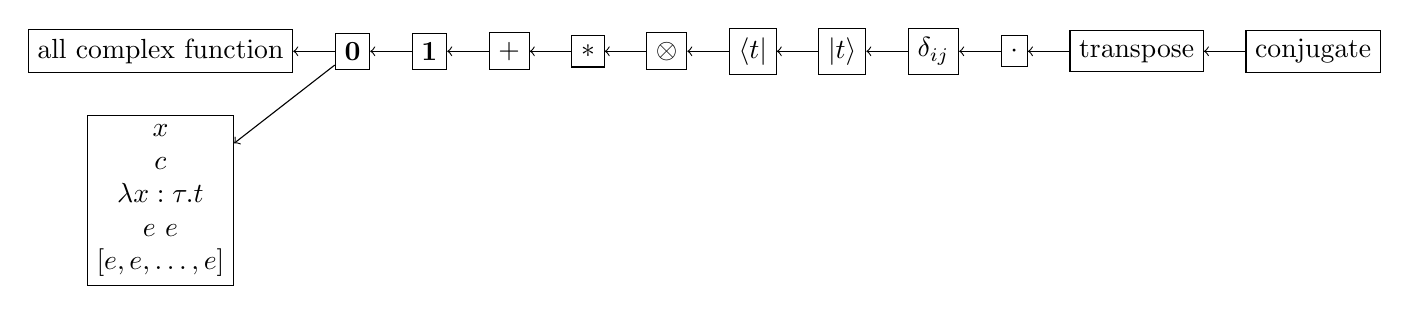
\begin{tikzpicture}[node distance=15pt]
    \node[draw]                     (complex) {all complex function};
    \node[draw, below= of complex, align=center] (STLC) {$x$\\$c$\\$\lambda x : \tau . t$\\$e\ e$\\$[e, e, \dots, e]$};

    \node[draw, right=of complex]                        (zero)   {$\mathbf{0}$};
    \node[draw, right=of zero]     (one)     {$\mathbf{1}$};
    \node[draw, right=of one]        (add)  {$+$};
    \node[draw, right=of add]         (scalar)  {$*$};
    \node[draw, right=of scalar]     (tensor)  {$\otimes$};
    \node[draw, right=of tensor]       (bra) {$\bra{t}$};
    \node[draw, right=of bra]       (ket) {$\ket{t}$};
    \node[draw, right=of ket]     (delta)     {$\delta_{ij}$};
    \node[draw, right=of delta]       (mul)  {$\cdot$};
    \node[draw, right=of mul]     (trans)     {transpose};
    \node[draw, right=of trans]     (conj)     {conjugate};

    
    \graph{
      (conj) -> (trans) -> (mul) -> (delta) -> (ket) -> (bra) -> (tensor) -> (scalar) ->(add) -> (one) -> (zero) -> (complex);
      (zero) -> (STLC);
    };
  \end{tikzpicture}
  \end{center}
\end{lemma}

\begin{proof}
  We need to check that every reduction rule makes the term strictly smaller in the LPO.
  Most cases are direct by definition. It's worth noting that for associative symbols $\cdot$, $\otimes$ and $+$, the simpler form is left-most associative, which is consistent with the LPO definition, because the right most subterms are compared first in \textbf{(LPO2c)}. Besides, $+$ is commutative, and the side condition of the subterm order helps avoid the infinite loop of rewriting.
\end{proof}


\begin{example}
  Important local confluence:
  \begin{center}
    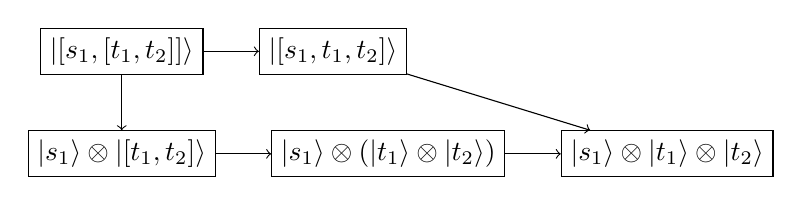
\begin{tikzpicture}[node distance=20pt]
      \node[draw] (P) {$\ket{[s_1,[t_1, t_2]]}$};
      \node[draw, right=of P]  (Q1)   {$\ket{[s_1, t_1, t_2]}$};
      \node[draw, below=of P]  (Q2)   {$\ket{s_1} \otimes \ket{[t_1, t_2]}$};

      \node[draw, right=of Q2]  (Q3)   {$\ket{s_1} \otimes (\ket{t_1} \otimes \ket{t_2})$};
      \node[draw, right=of Q3]  (Q4)   {$\ket{s_1} \otimes \ket{t_1} \otimes \ket{t_2}$};


      \graph{
        (P) -> (Q1) -> (Q4);
        (P) -> (Q2) -> (Q3) -> (Q4);
      };
    \end{tikzpicture}
  \end{center}
\end{example}

\begin{claim}[Normal Form]
  The normal form $NF$ of Dirac notations should approximately be like:
  \begin{align*}
    NF ::=&\ \mathbf{0}_{\tau, \sigma}\ |\ \sum (c*\delta\otimes\delta\otimes \cdots \otimes \delta \otimes OPT \otimes OPT \otimes \cdots \otimes OPT) \\
    OPT ::=& \ket{\cdot} \otimes \ket{\cdot} \otimes \cdots \otimes \ket{\cdot} \otimes \bra{\cdot} \otimes \bra{\cdot} \otimes \cdots \otimes \bra{\cdot}\ |\ X
  \end{align*}
\end{claim}

$\ket{\cdot}$ represents ket-like terms and $\bra{\cdot}$ represents bra-like terms.


\clearpage


\subsection{Labelled Dirac Notation}

\begin{definition}[quantum register]
  $$
  r ::= E\ |\ x\ |\ (r, r)
  $$
  Here $E$ is the terminal symbol for empty register and $x$ is a quantum variable.
\end{definition}

\begin{definition}[quantum variable typing]
  The typing for quantum variable $x$ is written as $x : T$, where $T$ is a space type.
\end{definition}

\begin{definition}[quantum context]
  The quantum contexts are ordered list of quantum variable typings, written as $\Gamma = [x : T; y : U; \dots]$. The empty context is denoted by $[]$.
\end{definition}

\begin{definition}[well-formed context]
  A well-formed context $\Gamma$, written as $\mathcal{WF}(\Gamma)$, is a context where variables appear uniquely. In other words, they are defined as:
  $$
  \frac{}{\mathcal{WF}([])}
  \qquad
  \frac{\mathcal{WF}(\Gamma)\qquad x \notin \Gamma}{\mathcal{WF}(\Gamma :: (x : T))}
  $$
\end{definition}


\begin{definition}[well-typed quantum register]
  Within a well-formed context $\mathcal{WF}(\Gamma)$, the well-typed quantum register is denoted as $\mathcal{WF}(\Gamma) \vdash r : T$, where $r$ denotes a quantum register and $T$ a space type. The well-typed quantum register is defined as follows.
  \begin{gather*}
  \frac{\mathcal{WF}(\Gamma)}{\mathcal{WF}(\Gamma) \vdash E : \texttt{Unit}}
  \qquad
  \frac{\mathcal{WF}(\Gamma)\qquad x:T \in \Gamma}{\mathcal{WF}(\Gamma) \vdash x : T}\\
  \ \\  
  \frac{\mathcal{WF}(\Gamma) \vdash r_1 : T_1 \qquad \mathcal{WF}(\Gamma) \vdash r_2 : T_2\qquad \mathcal{WF}(\Gamma) \vdash r_1 \| r_2}{\mathcal{WF}(\Gamma) \vdash (r_1, r_2) : (T_1 * T_2) }
  \end{gather*}
  Note that $\mathcal{WF}(\Gamma) \vdash r_1 \| r_2$ is defined below.
\end{definition}


\begin{definition}[atomic quantum register]
  We say a quantum register $r$ is atomic in context $\Gamma$ if we can prove
  $\mathcal{WF}(\Gamma) \vdash r : A$, where $A$ is a atomic type.
\end{definition}

\begin{definition}[quantum subsystem]
  A quantum subsystem $S$ is a set of quantum registers. 
  We say it's a well-formed quantum subsystem in context $\Gamma$ if all the elements are atomic quantum register in $\Gamma$. 
  For a quantum register $r$, $\mathrm{set}(\Gamma, r)$ represents the corresponding well-typed quantum subsystem in $\Gamma$.
  Two quantum registers are disjoint in $\Gamma$, written as $\mathcal{WF}(\Gamma) \vdash r_1 \| r_2$, if the corresponding quantum subsystems are disjoint.
\end{definition}
\textbf{Remark:} The description of quantum subsystem still need refinement.

\begin{definition}[labelled Dirac notation]
    Labelled Dirac notation is defined by:
    $$
    e ::= e_d [r_k; r_b]\ |\ e + e\ |\ e * e\ |\ e \otimes e\ |\ e^*\ |\ e^T.
    $$
    Here $e_d$ is a Dirac notation and $r_k, r_b$ are quantum registers.
\end{definition}

\begin{definition}[labelled notation typing]
  A typing of labelled Dirac notation $e$ in well-formed context $\Gamma$ is written as $\mathcal{WF}(\Gamma) \vdash e : (S_k, S_b)$, where $S_k$ and $S_b$ are quantum subsystems. 
\end{definition}

\begin{definition}[well-typed labelled Dirac notation]
  For the typing of labelled Dirac notation $\mathcal{WF}(\Gamma) \vdash e : (T_k, T_b)$, the well-typed proof is defined by
  \begin{gather*}
    \frac{\vdash e_d : (T_k, T_b) \qquad \mathcal{WF}(\Gamma) \vdash r_k : T_k \qquad \mathcal{WF}(\Gamma) \vdash r_b : T_b}{\mathcal{WF}(\Gamma) \vdash e_d[r_k; r_b] : (\mathrm{set}(\Gamma, r_k), \mathrm{set}(\Gamma, r_b))}\\
    \ \\
    \frac{\mathcal{WF}(\Gamma) \vdash e_1 : (S_k, S_b) \qquad \mathcal{WF}(\Gamma) \vdash e_2 : (S_k, S_b)}{\mathcal{WF}(\Gamma) \vdash e_1 + e_2 : (S_k, S_b)}\\
    \ \\
    \frac{\mathcal{WF}(\Gamma) \vdash e_1 : (S_k, S_b) \qquad \mathcal{WF}(\Gamma) \vdash e_2 : (S_k', S_b')
    \qquad S_k \cap (S_k' - S_b) = \emptyset
    \qquad (S_b - S_k') \cap S_b' = \emptyset}
    {\mathcal{WF}(\Gamma) \vdash e_1 * e_2 : (S_k \cup (S_k' - S_b), (S_b - S_k') \cup S_b')}\\
    \ \\
    \frac{\mathcal{WF}(\Gamma) \vdash e_1 : (S_k, S_b) \qquad \mathcal{WF}(\Gamma) \vdash e_2 : (S_k', S_b')
    \qquad S_k \cap S_k' = \emptyset
    \qquad S_b \cap S_b' = \emptyset}
    {\mathcal{WF}(\Gamma) \vdash e_1 \otimes e_2 : (S_k \cup S_k', S_b \cup S_b')}\\
    \ \\
    \frac{\mathcal{WF}(\Gamma) \vdash e : (S_k, S_b)}{\mathcal{WF}(\Gamma) \vdash e^* : (S_k, S_b)}
    \qquad
    \frac{\mathcal{WF}(\Gamma) \vdash e : (S_k, S_b)}{\mathcal{WF}(\Gamma) \vdash e^T : (S_b, S_k)}
  \end{gather*}
\end{definition}

\begin{definition}[labelled Dirac notation reduction]
  We consider the reduction on typings of labelled Dirac notations. The rules are defined by:
  \begin{gather*}
    \mathcal{WF}(\Gamma) \vdash ((e_d + e_d')[r_k; r_b]: (S_k, S_b)) \to (e_d[r_k; r_b] + e_d'[r_k; r_b] : (S_k, S_b))\\
    \cdots
  \end{gather*}
\end{definition}

\begin{claim}[well-typing preservation]
  Reduction on labelled notation typings preserve the well-typed proof. That is,
  $$
  \forall e \forall \Gamma, \mathcal{WF}(\Gamma) \vdash (e : (S_k, S_b)) \to (e' : (S_k, S_b)),
  $$
  and
  $$
  \mathcal{WF}(\Gamma) \vdash e : (S_k, S_b)\ \textrm{and}\ \mathcal{WF}(\Gamma) \vdash (e : (S_k, S_b)) \to (e' : (S_k, S_b))\ \textrm{imples}\ \mathcal{WF}(\Gamma) \vdash e' : (S_k, S_b).
  $$
\end{claim}


\section{Modularising Dirac Notation by Category}
In consideration of the complicated depnedency of different parts of the Dirac notation theory, expressing it in a modularised manner makes it more clear, organized and easy to extend. In Coq, the implementations follow this design by \textit{Module} and \textit{Module Types}. We can speak in category theory for the same purpose in theory developement.



\section{About Big Operators and Lambda Calculus}
I believe the two vital considerations for big operators are \textbf{lambda calculus} and \textbf{set syntax}. We have to include lambda calculus, because the expression for big operators are essentially functions. And for sets with certain syntax, it is possible to design a complete term rewriting system.

Assume the index of big operator has type $T$, then a set of index values can be considered as functions of $T \to \texttt{bool}$.

\begin{example}[big-op lifting]
  We can consider how to extend a term rewriting system $R$ with big operators.

  \begin{enumerate}
    \item Consider a simply typed lambda calculus, where functions in $R$ appear as constants in the calculus.
    \item Pick out an associative bineary function symbol $+$.
    \item Pick out the neuteral element so that $0 + a \to a$.
    \item Define the type $T$ as type of indices.
    \item Define the type $\texttt{set} : T \to \texttt{Type}$ as the sets.
    \item The big operator is a constant $\sum : \texttt{set}\ T \to (T \to U) \to U$, where $U$ is the type of the big operator expression.
  \end{enumerate}
\end{example}


\begin{example}
  Assume sets are constructed by enumerating $T$ terms, then the syntax with big operators is still decidable.
\end{example}

May be the sets of integer intervals $[m, n]$ are worth considering. But I don't believe it can be decidable in more general cases.



\subsection{Lineal with Sum}

The language of \textit{vectors} is a three-sorted language, with the sorts for vectors, scalars and sets, described by the following term grammar:

$$
t ::=\ x\ |\ \lambda x\ t\ |\ t\ t\ |\ \mathbf{0}\ |\ \alpha.t\ |\ t + t\ |\ \sum_{x \in S} t
$$

Here $\sum_{x \in S} t$ can be considered as a special abstraction, where $x$ is the bound variable for index and $S$ is the set of index values for summation.

\begin{definition}[The system Sum]
    \begin{align*}
        & \sum_{x \in S} \mathbf{0} \to \mathbf{0} \\
        & \alpha.\sum_{x \in S} u \to \sum_{x \in S} \alpha.u \\
        & \sum_{x \in S} u + \sum_{x \in S} v  \to \sum_{x \in S} (u + v) \\
        \tag{*}
        & u\ \sum_{x \in S} v \to \sum_{x \in S} (u\ v)\\
        \tag{**}
        & \sum_{x \in S} \sum_{y \in T} u = \sum_{y \in T} \sum_{x \in S} u
    \end{align*}
(*)\ This makes sense because abstractions are linear in lineal.\\
(**)\ Requires that $T$ is not dependent on $x$.

And sum is not considered as a base vector.
\end{definition}



\section{Tuple, Variable Index and Separation Logic}

\subsection{Motivating example}

Consider the notation:
$$
\texttt{CX}[a[i], a[j]] = \texttt{H}[a[j]]\ \texttt{CZ}[a[i], a[j]]\ \texttt{H}[a[j]]
$$
where $a$ is a quantum tuple register. The equality seems to hold, but here is a precondition: $i \neq j$. Otherwise, the Dirac notation is not even well-typed. 

Because we only consider well-typed Dirac notations, we use separation logic to deal with these precondition on well-typed proofs.





\section{Other Examples}

This section collects typical examples for Dirac notation syntax and equality.

\begin{example}
  $$
  \sum_{k=0}^{N-1} e^{\frac{2\pi i j k}{N}}\ket{k}
  $$
  Assume $t$ and $b$ are bit strings.
  $$
  \frac{1}{\sqrt{2^n}} \sum_t (-1)^{\sum_i b_i \cdot t_i} \ket{t}_{\bar{x}}
  $$\end{example}
This example requires
\begin{itemize}
  \item big-op of sum (index in vector term and coefficent).
\end{itemize}
This example clearly shows that the linear algebra module is dependent on the quantum term and type. For example, here $\sum_i b_i \cdot t_i$ should be considered as a quantum term, but the whole expression $(-1)^{\sum_i b_i \cdot t_i}$ is a complex number term.



\begin{example}
  $$
  \bigotimes_{i = 0}^{k-1} \ket{0}_{x_i}
  $$
  $$
  \left ( \bigotimes_{i = 0}^{k-1} \texttt{QFT}[x_i] \right ) \ket{0}_{\bar{x}}
  $$
\end{example}
This example requires 
\begin{itemize}
  \item tuple of quantum variable, variable indices,
  \item big-op of tensor (index in quantum tuple).
\end{itemize}

\begin{example}
  Assume $U$ is a unitary transform,
  $$
  \frac{1}{\sqrt{2^t}} \sum_{j=0}^{2^t-1} \ket{j} U^j \ket{u}
  $$
\end{example}
This example requires
\begin{itemize}
  \item integer index and power of operators,
  \item big-op of sum (index in the exponent).
\end{itemize}

\begin{example}
  $$
  \sum_{s=0}^{r-1} \sum_{j=0}^{2^t-1} e^{\frac{2\pi i s j}{r}} \ket{j} \ket{u_s}
  $$
\end{example}
This example requires
\begin{itemize}
  \item nested big-op of sum.
\end{itemize}


\subsection{Equality Benchmark}

\begin{example}
  $$
  (U_{S_1} \otimes I_{S_2}) (\ket{\phi}_{S_1} \ket{\psi}_{S_2}) = (U_{S_1} \ket{\phi}_{S_1}) (I_{S_2}\ket{\psi}_{S_2}) = (U_{S_1} \ket{\phi}_{S_1}) \ket{\psi}_{S_2}
  $$
\end{example}
This example requires 
\begin{itemize}
  \item type variables, the universal quantification on type $T$:
    $$
    \forall (T : \texttt{qType}) (U : (T, T)) (S_1 : T), \dots
    $$
  \item quantum variables,
  \item vector and linear operator variables.
\end{itemize}

\begin{example} [ParaHadamard]
  $$
  (\bigotimes_i^n H_{x_i}) \ket{b}_{\bar{x}} = \frac{1}{\sqrt{2^n}} \sum_t (-1)^{\sum_i b_i t_i} \ket{t}_{\bar{x}}
  $$
\end{example}

% 
\chapter{20231117}

\section{Introduction}

Say we want a theory about formalizing Dirac notations. We want it to be as expressive and general as possible, while stay highly automated at the same time. One difficulty is that there are so many factors to consider: quantum registers and variables, indexes, big operators, the theory for natural and complex numbers, whether it is more like a theorem prover or a solver... 

Generally speaking, there is a dilemma between automation and expressiveness. Consider the two extreme cases: we can assume that the natural/real numbers correspond to those constants stored in the computer. Then we can get rid of the decidability problems about numbers. It will be easy to implement and use, but with very limitted applicability, which makes it more like a solver. On the other hand, the whole thery of Dirac notations can be developed based on expressive logic basis (e.g., Coq). In this case, we can have complicated terms about those numbers, and even the scale of quantum system can be parameterized. But the deductions in this setting is much harder and the tool will be more like a theorem prover.

It's hard to say which is the best choice. If the implementation is restricted to very limited cases (i.e., not general enough), it will not be theoretically intersting. And if the theory is too general, it will be hard to implement a corresponding practical tool, and such tools will be complicated and hard to use.

In front of this situation, it seems that we need to make a decision before developming the theory and work on the implementation. But the better approach exists: one obvious conclusion is, that the ability of Dirac notation system is dependent on its basis. We can study the theory for Dirac notations with respect to different basis.
This basis include the logic and methodology of reasoning, how natural/complex numbers are represented and reasoned about, as well as those stuff about sets. 

In other words, here we consider the Dirac notation theory as a functor. (See the Coq implementation for functors: \url{https://coq.inria.fr/refman/language/core/modules.html\#typing-modules})

The implementation in Python loyally reflects the theory described in this draft. To address the problem of \textit{put formal systems into Python as it is}, I designed the methodology and framework called REM (Reliable Encoding Mechanism), which is a set of concrete discipline to practise CH-correspondence in Python language. The Dirac notation theory implementation as a functor is developped with this framework. I did experiments on different basis theories(tools): Python numerical complex numbers and computer algebra system by \textit{Wolfram Engine}.
However, the flexibility of this implementation also means the low efficiency. Therefore this can be considered as a prototype for theory verification purpose.


\section{Preliminaries}

\subsection{Reduction in Mathematica}

\subsection{Clarification}
There are a few concepts to be clarified here.

\subsubsection*{Quantum Type/Term}
The basis theory $\mathfrak{T}$ contains the information about quantum types and terms, which further determine the possible types and basis of Hilbert spaces. The type of every Hilbert space is specified by a type $T$ in $\mathfrak{T}$, and the basis of the Hilbert space consists of the legal terms $t$ of type $T$. Notice that in casual reasoning about Dirac notations, people only care about the dimension of Hilbert spaces. Here our type is richer then dimension only, and we adopt the strict type checker $\mathfrak{T} \Vdash t : T$ which distinguishes Hilbert spaces of different types.


\subsubsection*{Quantum Variable}
Quantum variables refer to the variables of Hilbert spaces. Every quantum variable $x$ has a classical type $T$ (provided by basis theory $\mathfrak{T}$), written as $x : T$, and it is called a \textbf{quantum variable typing}. The variable's type is exactly that of the Hilbert space it represents. And in L1A Dirac notations, we will consider the environment of definitions and substitutions of quantum variables.

\subsubsection*{Quantum Variable Context}
A quantum variable context is an ordered sequence of quantum variable typings, denoted by $\Gamma = [x_1 : T_1; x_2 : T_2; \dots]$. The well-typed proof of Dirac notations is considered with respect to a quantum variable context. A well-typed quantum variable context is denoted by $\mathcal{WF}(\Gamma)$.

\subsubsection*{Quantum Subsystem}
A quantum subsystem treated as a set of ``atomic'' quantum system, and disjointness between subsystems corresponds to disjointness of these sets. For L0 Dirac notations, quantum subsystems are simply enumeration of quantum variables, so there is no hardness in disjointness decision. However, for L1C Dirac notations, we will have quantum arrays, which makes the problems very nasty.

\subsubsection*{Quatum Register}
Quantum registers are expressions (i.e., terms) of Hilbert spaces. They are used as the labels for Dirac notations. Quantum registers can be quantum variables or pairs. Quantum registers have their types, which is also the type of the Hilbert space they evaluate to. A well-typed quantum register is represented by $\mathcal{WF}(\Gamma) \vdash r : T$.

\textbf{Notice:} For $\mathcal{WF}(\Gamma) \vdash r_1 : T_1$ and $\mathcal{WF}(\Gamma) \vdash r_2 : T_2$, the register pair $r_1, r_2$ has the product type $T_1 * T_2$, and evaluates to the tensor subsystem of $r_1$ and $r_2$. In other words, the pair in classical type, the pair register and the tensor of subsystems are closely related. This is reflected in the typing and reduction rules.

\textcolor{red}{Other register structure?}
We may be able to design a correspondence between operation on classical terms and those on quantum variables. Pair structure is a case for it.


\section{L0 Dirac Notation}

\textbf{L0 Dirac notation} refers to the simplest theories of Dirac notations. There is no big-operators, no quantum arrays, no environments and definitions.

\subsection{Basis Theories}
For distinguishability, the reasoning in basis theories is represented by $\Vdash$.

\begin{definition}[L0 classical type theory]
  A \textbf{L0 classical type theory} $\mathfrak{T}$ is a formal system containing the following definitions:
  \begin{itemize}
    \item the sort \texttt{Type}, types $T$ and term $t$,
    \item the well-typed relation $\mathfrak{T} \Vdash T : \texttt{Type}$ and $\mathfrak{T} \Vdash t : T$,
    \item the equality of terms $\mathfrak{T} \Vdash t1 = t2$.
  \end{itemize}
\end{definition}

\begin{definition}[L0 complex number theory]
  A \textbf{L0 complex number theory} $\mathfrak{C}$ is a formal system containing the following definitions:
  \begin{itemize}
    \item the type $\mathbb{C}$, the well-typed relation $\mathfrak{C} \Vdash c : \mathbb{C}$.
  \end{itemize}
\end{definition}

\subsection{Notations}

\begin{definition}[L0 quantum register]
  A \textbf{L0 quantum register} can be built in two ways:
  \begin{itemize}
    \item a quantum variable $r$,
    \item a pair register $r_1, r_2$.
  \end{itemize}
\end{definition}

\begin{definition}[L0 Dirac notation]
  The grammar for \textbf{L0 Dirac notation} is:
  $$
  e ::=\ c\ |\ \textbf{0}_{S_K, S_B}\ |\ \ket{v}_r\ |\ \bra{v}_r\ |\ M_{r_1, r_2}\ |\ e + e\ |\ e * e\ |\ e \otimes e\ |\ e^\dagger.
  $$
  Here $c$ is the complex number term in $\mathfrak{C}$. $S_K$ and $S_B$ are quantum subsystems. $v$ is the classical term in $\mathfrak{T}$. $r$ is the quantum register. Especially, $M_{r_1, r_2}$ represents a variable of Dirac notation.
\end{definition}

\begin{definition}[well-typed quantum register]
  We say $r$ is a \textbf{well-typed quantum register} in context $\Gamma$ if we can prove $\mathcal{WF}(\Gamma) \vdash r : T$ for some $T$.
\end{definition}

\begin{definition}[well-typed Dirac notation]
  We say $e$ is a \textbf{well-typed Dirac notation} in context $\Gamma$ if we can prove $\mathcal{WF}(\Gamma) \vdash e : (S_K, S_B)$ for some $S_K$ and $S_B$.
\end{definition}

\subsection{Typing rules}

\subsubsection*{well-formed context}

$$
\frac{}{\mathcal{WF}([])}
\qquad 
\frac{\mathcal{WF}(\Gamma)\qquad \mathfrak{T}\Vdash T : \texttt{Type}\qquad x \notin \Gamma}{\mathcal{WF}(\Gamma; x : T)}
$$

\subsubsection*{well-typed quantum registers}
$$
\frac{\mathcal{WF}(\Gamma)\qquad x:T \in \Gamma}{\mathcal{WF}(\Gamma) \vdash x : T}
\qquad
\frac{\mathcal{WF}(\Gamma)\vdash a : T\qquad \mathcal{WF}(\Gamma) \vdash b : U \qquad a \| b}{\mathcal{WF}(\Gamma) \vdash a, b : T * U}
$$

Here $a \| b$ means that the quantum subsystems of $a$ and $b$ are disjoint.

\subsubsection*{well-typed Dirac notations}
\begin{gather*}
  \frac{}{\mathcal{WF}(\Gamma)\vdash c : (\emptyset, \emptyset)} \\
  \ \\
  \frac{}{\mathcal{WF}(\Gamma)\vdash \textbf{0}_{S_K, S_B} : (S_K, S_B)}\\
  \ \\
  \frac{\mathcal{WF}(\Gamma)\vdash r : T \qquad \mathfrak{T} \Vdash v : T}{\mathcal{WF}(\Gamma)\vdash \ket{v}_r : (set(r), \emptyset)}\\
  \ \\
  \frac{\mathcal{WF}(\Gamma)\vdash r : T \qquad \mathfrak{T} \Vdash v : T}{\mathcal{WF}(\Gamma)\vdash \bra{v}_r : (\emptyset, set(r))}\\
  \ \\
  \frac{}{\mathcal{WF}(\Gamma)\vdash M_{r_1, r_2} : (set(r_1), set(r_2))}\\
  \ \\
  \frac{\mathcal{WF}(\Gamma)\vdash e_1 : (S_K, S_B)\qquad \mathcal{WF}(\Gamma)\vdash e_2 : (S_K, S_B)}{\mathcal{WF}(\Gamma)\vdash e_1 + e_2 : (S_K, S_B)}\\
  \ \\
  \frac{\mathcal{WF}(\Gamma)\vdash e_1 : (S_K, S_B)\qquad \mathcal{WF}(\Gamma)\vdash e_2 : (S_K', S_B')\qquad S_K \cap (S_K'-S_B) = \emptyset\qquad (S_B-S_K')\cap S_B' = \emptyset}{\mathcal{WF}(\Gamma)\vdash e_1 * e_2 : (S_K \cup (S_K' - S_B), (S_B-S_K') \cup S_B')}\\
  \ \\
  \frac{\mathcal{WF}(\Gamma)\vdash e_1 : (S_K, S_B)\qquad \mathcal{WF}(\Gamma)\vdash e_2 : (S_K', S_B')\qquad S_K \cap S_K= \emptyset\qquad S_B\cap S_B' = \emptyset}{\mathcal{WF}(\Gamma)\vdash e_1 \otimes e_2 : (S_K \cup S_K', S_B \cup S_B')}\\
  \ \\
  \frac{\mathcal{WF}(\Gamma)\vdash e : (S_K, S_B)}{\mathcal{WF}(\Gamma)\vdash e^\dagger : (S_B, S_K)}
\end{gather*}

In fact, all the Dirac notations have their corresponding \textit{tensor network} interpretations, and these typing rules are very intuitive in this point of view.

We can understand the tensor $e_1 \otimes e_2$ as \textit{stacking two individual nodes}.

We can understand the multiplication $e_1 * e_2$ as \textit{contracting all possible corresponding indices between two nodes}.

\section{Deciding L0 Dirac Notation}

\textcolor{red}{How to develop a convergent term rewriting system? And what is the requirement on the basis theories?}

\vspace{1em}

One problem is that we have well-typed side conditions for rerwriting rules. In consideration of this, I feel that what we need is a term rewriting system for \textbf{well-typed proof of Dirac notations}, instead of Dirac notation alone.

\vspace{1em}
Because we have AC functions ($e_1 + e_2$ and $e_1 \otimes e_2$), we will need a reduction order, which is defined as follows.

\begin{definition}[Dirac notation order]
  The order $e_1 < e_2$ is defined by:
  \begin{gather*}
    \frac{e \neq \textbf{0}_{S_K, S_B}\qquad e \neq c}{e < c}\\
    \ \\
    \frac{r < s}{\ket{v}_r < \ket{u}_s} \qquad \frac{r < s}{\ket{v}_r < \bra{u}_s}\qquad \frac{r < s}{\bra{v}_r < \ket{u}_s}\qquad \frac{r < s}{\bra{v}_r < \bra{u}_s}\\
    \ \\
    \frac{}{\bra{v}_r < \ket{u}_r} \\
    \ \\
    \frac{\mathfrak{T} \Vdash v < u}{\ket{v}_r < \ket{u}_r}\qquad\frac{\mathfrak{T} \Vdash v < u}{\bra{v}_r < \bra{u}_r}\\
    \ \\
    \frac{}{M[a, b] < \ket{v}_r}\qquad \frac{}{M[a, b] < \bra{v}_r}\\
    \ \\
    \frac{a < s}{M[a, b]<N[s, t]}\qquad \frac{b < t}{M[a, b]<N[a, t]}\qquad \frac{M < N}{M[a, b] < N[a, b]}\\
    \ \\
    \frac{}
    \ \\
    \frac{e_2 < e}{e_1 + e_2 < e}\qquad \frac{e_2 < e}{e_1 * e_2 < e} \qquad \frac{e_2 < e}{e_1 \otimes e_2 < e}
  \end{gather*}
\end{definition}

\textcolor{red}{The ``order'' results from intuition and experiments, and I haven't considered whether it's legal for termination proof.}

\subsection{Reduction rules}
The reduction rules for L0 Dirac notation are presented below. This term rewriting system is denoted as $\textbf{L0}$.


\subsubsection*{Register Decomposition}
\begin{align*}
  & \vdash \ket{v_1, v_2}_{r_1, r_2} \to \ket{v_1}_{r_1} \otimes \ket{v_2}_{r_2} \qquad \vdash \bra{v_1, v_2}_{r_1, r_2} \to \bra{v_1}_{r_1} \otimes \bra{v_2}_{r_2} 
\end{align*}

\subsubsection*{Complex Number}
\begin{align*}
  & \vdash 0 \to \textbf{0}_{\emptyset, \emptyset}\\
  & \vdash c_1 + c_2 \to c_1 + c_2\qquad \text{(the addition of complex numbers)}\\
  & \vdash c_1 \otimes c_2 \to c_1 * c_2\qquad \text{(the multiplication of complex numbers)}\\
  & \vdash c_1 \otimes e + c_2 \otimes e \to (c_1 + c_2) \otimes e\\
  & \vdash 1 \otimes e \to e\\
  & \vdash c^\dagger \to conj(c)
\end{align*}

\subsubsection*{Zero Operator}
Consider the syntax $\textbf{0}_{S_K, S_B}$. It is ugly to put quantum subsystems $S_K$ and $S_B$ into the syntax, but they are necessary for now: they are required in reduction rules, and the well-typed proof for $\textbf{0}$ alone is not unique.

However, it is true that in most cases the quantum subsystems can be determined by unification, and therefore it may be a good idea to reason about well-typed proofs of Dirac notations like a typing system. However, this introduces another problem: do we allow variables of types for Dirac notations?

\begin{align*}
  & \vdash \textbf{0}_{S_K, S_B} + e \to e
  \qquad \vdash e + \textbf{0}_{S_K, S_B} \to e\\
  &\ \\
  & \frac{\mathcal{WF}(\Gamma)\vdash e : (S_K', S_B')}{\textbf{0}_{S_K, S_B} * e \to \textbf{0}_{S_K \cup (S_K' - S_B), (S_B-S_K') \cup S_B'}}
  \qquad \frac{\mathcal{WF}(\Gamma)\vdash e : (S_K, S_B)}{e * \textbf{0}_{S_K', S_B'} \to \textbf{0}_{S_K \cup (S_K' - S_B), (S_B-S_K') \cup S_B'}}\\
  &\ \\
  & \frac{\mathcal{WF}(\Gamma)\vdash e : (S_K', S_B')}{\textbf{0}_{S_K, S_B} \otimes e \to \textbf{0}_{S_K \cup S_K', S_B \cup S_B'}}
  \qquad \frac{\mathcal{WF}(\Gamma)\vdash e : (S_K, S_B)}{e \otimes \textbf{0}_{S_K', S_B'} \to \textbf{0}_{S_K \cup S_K', S_B \cup S_B'}}\\
  &\ \\
  & \vdash \textbf{0}_{S_K, S_B}^\dagger \to \textbf{0}_{S_B, S_K}
\end{align*}

\subsubsection*{Addition}
\begin{align*}
  & \vdash e_1 + (e_2 + e_3) \to e_1 + e_2 + e_3 \\
  & e_1 < e_2 \vdash e_1 + e_2 \to e_2 + e_1
\end{align*}

\subsubsection*{Tensorization}
These rules try to lift $e_1 \otimes e_2$ above $e_1 * e_2$ structures when possible, which is closer to the desired normal form. But I am not sure whether these rules are complete for this purpose. Especially, the (\ref{rule: tmt}) rule seems artificial.
\begin{align*}
  & \frac{\mathcal{WF}(\Gamma)\vdash e_1 : (S_1, S_1')\quad \mathcal{WF}(\Gamma)\vdash e_3 : (S_3, S_3')\quad S_1' \cap S_3 = \emptyset}
  {e_1 * (e_2 \otimes e_3) \to (e_1 * e_2) \otimes e_3} \\
  &\ \\
  & \frac{\mathcal{WF}(\Gamma)\vdash e_1 : (S_1, S_1')\quad \mathcal{WF}(\Gamma)\vdash e_2 : (S_2, S_2')\quad S_1' \cap S_2 = \emptyset}
  {e_1 * (e_2 \otimes e_3) \to e_2 \otimes (e_1 * e_3)} \\
  &\ \\
  & \frac{\mathcal{WF}(\Gamma)\vdash e_2 : (S_2, S_2')\quad \mathcal{WF}(\Gamma)\vdash e_3 : (S_3, S_3')\quad S_2' \cap S_3 = \emptyset}
  {(e_1 \otimes e_2) * e_3 \to (e_1 * e_3) \otimes e_2} \\
  &\ \\
  & \frac{\mathcal{WF}(\Gamma)\vdash e_1 : (S_1, S_1')\quad \mathcal{WF}(\Gamma)\vdash e_3 : (S_3, S_3')\quad S_1' \cap S_3 = \emptyset}
  {(e_1 \otimes e_2) * e_3 \to e_1 \otimes(e_2* e_3)} \\
  &\ \\
  & \frac{\mathcal{WF}(\Gamma)\vdash e_1 : (S_1, S_1')\qquad \mathcal{WF}(\Gamma)\vdash e_2 : (S_2, S_2')\qquad S_1' \cap S_2 = \emptyset}
  {e_1 * e_2 \to e_1 \otimes e_2}\\
  &\ \\
  & \frac{
    \begin{aligned}
      & \mathcal{WF}(\Gamma) \vdash e_1 : (S_1, S_1')\qquad & \mathcal{WF}(\Gamma) \vdash e_4 : (S_4, S_4') \qquad & S_1' \cap S_4 = \emptyset\\
      & \mathcal{WF}(\Gamma) \vdash e_2 : (S_2, S_2') & \mathcal{WF}(\Gamma) \vdash e_4 : (S_4, S_4')\qquad & S_2' \cap S_3 = \emptyset
    \end{aligned}
  }{(e_1 \otimes e_2) * (e_3 \otimes e_4) \to (e_1 * e_3) \otimes (e_2 * e_4)} \tag{*} \label{rule: tmt}
\end{align*}

\subsubsection*{Multiplication}
\begin{align*}
  & \vdash e_1 * (e_2 * e_3) \to e_1 * e_2 * e_3\\
  & \vdash e_1 * (e_2 + e_3) \to e_1 * e_2 + e_1 * e_3
  \qquad \vdash (e_1 + e_2) * e_3 \to e_1 * e_3 + e_2 * e_3\\
  & \vdash \bra{i}_r * \ket{j}_r \to \delta_{ij}
\end{align*}

\subsubsection*{Tensor}
\begin{align*}
  & \vdash e_1 \otimes (e_2 + e_3) \to e_1 \otimes e_2 + e_1 \otimes e_3
  \qquad \vdash (e_1 + e_2) \otimes e_3 \to e_1 \otimes e_3 + e_2 \otimes e_3\\
  & \vdash e_1 \otimes (e_2 \otimes e_3) \to e_1 \otimes e_2 \otimes e_3\\
  & e_1 < e_2 \vdash e_1 \otimes e_2 \to e_2 \otimes e_1
\end{align*}

\subsubsection*{Conjugate Transpose}
\begin{align*}
  & \vdash \ket{v}_r^\dagger \to \bra{v}_r \qquad \vdash \bra{v}_r^\dagger \to \ket{v}_r\\
  & \vdash (e_1 + e_2)^\dagger \to e_1^\dagger + e_2^\dagger \qquad \vdash (e_1 * e_2)^\dagger \to e_2^\dagger * e_1^\dagger \qquad \vdash (e_1 \otimes e_2)^\dagger \to e_1^\dagger \otimes e_2^\dagger
\end{align*}
  
  
The convergent proof of the reduction system is dependent on the order. Moreover, the efficiency of the reduction algorithm is also partially limited by the order. Therefore to optimize the algorithm, more effort is need to improve the reduction order and simplify the decending path.

\begin{figure}[h]
  \center
  \includegraphics*[width = 0.7 \textwidth]{fig/red_illustration.png}
  \caption{An example of normal form calculation.}
\end{figure}

\subsection{Properties}

\begin{lemma}
  The reduction rules in $\textbf{L0}$ preserve the well-typed property of Dirac notations.
\end{lemma}
\begin{proof}
  To be proved.
\end{proof}

\begin{theorem}
  The term rewriting system $\textbf{L0}$ is confluent.
\end{theorem}
\begin{proof}
  To be proved.
\end{proof}

\begin{theorem}
  If the reasonings in basis theories $\mathfrak{T}$ and $\mathfrak{C}$ are decidable, then so is the word problem for $\textbf{L0}$.
\end{theorem}
\begin{proof}
  To be proved.
\end{proof}


\section{L1A Dirac Notation}
\textbf{L1A Dirac notation} is L0 Dirac notation with definition, function and environment extensions.

Consider this notation:
$$
\left [\ket{+} := \texttt{fun x : bool => }\frac{\ket{0}_x + \ket{1}_x}{\sqrt{2}} \right ][\texttt{y : bool}] \vdash \bra{+}_y * \ket{+}_y = 1
$$
It's reasonable to have definitions for Dirac notations. For example, $\ket{+}$ and $\texttt{CX}$. I believe the appropriate way to express such definitions is through lambda expressions. Here's another example:

\begin{align*}
\texttt{CX := fun pair : bool * bool =>} & \texttt{ |0, 0>[pair]<0, 0| + |0, 1>[pair]<0, 1|}\\
& \texttt{+ |1, 1>[pair]<1, 0| + |1, 0>[pair]<1, 1|.}
\end{align*}

Of course, here \texttt{pair : bool * bool} does not mean \texttt{pair} is a classical term of $\texttt{bool * bool}$, but means \textit{\texttt{pair} is a quantum variable of \texttt{bool * bool} type}. (Maybe a different notation is needed here.)

Consistently, we will need environments for the definitions. We can even allow additional rewriting rules, which can be considered as the extra assumptions on variables. But this will make the implementation more like a theorem prover than a solver.


\section{L1B Dirac Notation}
\textbf{L1B Dirac notation} is L0 Dirac notation with big-operator extensions.

Consider this notation:
$$
\mathcal{WF}([r : \texttt{Seq bool n}]) \vdash \frac{1}{\sqrt{2^n}}\sum_{i \in \{0, 1\}^n} \ket{i}_r = \bigotimes_{i=0}^{n-1} \frac{\ket{0}_{r[i]} + \ket{1}_{r[i]}}{\sqrt{2}}.
$$

This example demonstrates a typical case of using big operators. Also, quantum arrays appear in the right hand side, which is almost always necessary when using big operators.



\section{L1C Dirac Notation}
\textbf{L1C Dirac notation} is L0 Dirac notation with quantum array extensions.

\subsection{Basis Theories}

\begin{definition}[L1C classical type system]
  A \textbf{L1C classical type system} $\mathfrak{T}$ is a L0 classical type system with the following extra definitions (mix-in):
  \begin{itemize}
    \item a type of natural numbers: $\mathfrak{T} \Vdash n : \mathbb{N}$,
    \item a type constructor \texttt{Seq} satisfying
    $$
    \frac{\mathfrak{T} \Vdash n : \mathbb{N}\quad \mathfrak{T} \Vdash T : \texttt{Type}}
    {\mathfrak{T} \Vdash \texttt{Seq}\ T\ n\ : \texttt{Type}}.
    $$
  \end{itemize}

\end{definition}


\section{L1D Dirac Notation}
\textbf{L1D Dirac notation} is L0 Dirac notation with other common operators, e.g. subtraction, conjugte and transpose.

\textcolor{red}{Maybe it's better to move conjugate/transpose to L0 and conjugate transpose to L1D?}


\section{L2 Dirac Notation}

L1 Dirac notations extends the simplest L0 theory in different perspectives.
And at some point, we will need to consider how to combine them to get even more powerful theories.

I believe there should be some ``confluent'' property between different L1 theories, so that they can work well with each other.

\section{Transplant Dirac Notation onto some CiC system}

This will help a lot in quantum formal verifications.

\section{Implementation}
\subsection{Reliable Encoding Mechanism}

A Python framework for the calculus of order-sorted universal algebra. Most formal systems can be embedded in such a universal algebra.



\bibliographystyle{plain}
\bibliography{ref}

\end{document}
